\documentclass[review]{elsarticle}
\DeclareGraphicsRule{.pdftex}{pdf}{*}{}
\usepackage{graphicx,color}
\usepackage{lineno,hyperref}
\usepackage{multirow}
\usepackage{verbatim}
\usepackage{appendix}
\usepackage{caption}
\usepackage{subcaption} %  for subfigures environments
\usepackage{tikz}
\usepackage{enumerate}

\pdfminorversion=7

%\modulolinenumbers[5]

\journal{Journal of Computational Physics}

%%%%%%%%%%%%%%%%%%%%%%%
%% Elsevier bibliography styles
%%%%%%%%%%%%%%%%%%%%%%%
%% To change the style, put a % in front of the second line of the current style and
%% remove the % from the second line of the style you would like to use.
%%%%%%%%%%%%%%%%%%%%%%%

%% Numbered
%\bibliographystyle{model1-num-names}

%% Numbered without titles
%\bibliographystyle{model1a-num-names}

%% Harvard
%\bibliographystyle{model2-names.bst}\biboptions{authoryear}

%% Vancouver numbered
%\usepackage{numcompress}\bibliographystyle{model3-num-names}

%% Vancouver name/year
%\usepackage{numcompress}\bibliographystyle{model4-names}\biboptions{authoryear}

%% APA style
%\bibliographystyle{model5-names}\biboptions{authoryear}

%% AMA style
%\usepackage{numcompress}\bibliographystyle{model6-num-names}

%% `Elsevier LaTeX' style
\bibliographystyle{elsarticle-num}
%%%%%%%%%%%%%%%%%%%%%%%

\graphicspath{./figures}

\begin{document}

\begin{frontmatter}

\title{Testing Flexi\tnoteref{mytitlenote}\ on Classic Riemann Problems}

\tnotetext[mytitlenote]{Flexi is Copyright (C) 2016, Prof.\ Claus-Dieter Munz and is released under the terms of the GNU General Public License v3.0. All files, scripts, and tools used to generate this report may be found in the \textbf{flexi/doc/flexiReport} directory within the NewFeatures branch of the Flexi github repository: \url{github.com/flexi-framework/flexi}. All references to a \textbf{directory} point to this location.}

%% Group authors per affiliation:
\author{R.\ W.\  Douglass\fnref{STRA}}

\author{G.\ A.\ Hansen\fnref{STRA}}
\address{STRA LLC, Los Alamos, NM \ USA}
%\fntext[myfootnote]{}

\fntext[STRA]{SciTech Research Associates, LLC, 1908 Deacon St, Los Alamos, New Mexico\  87544\  USA}

\begin{abstract}
Flexi\cite{flexigeneral} is a transient, multi-dimensional fluid dynamics simulation code framework using both the discontinuous Galerkin method and Finite Volume method for discretizing the equations of mass, momentum, and energy conservation. The results presented test Flexi's ability to simulate various challenging one- and two-dimensional Riemann problems with results compared to exact solutions whenever possible.  Although no attempt is made to optimize results through use of the many Flexi options, using the basic tutorial mesh and input files for the Sod problem was a good starting point.  All mesh and Flexi input decks are provided as well as detailed information regarding building the code, preparing the output for use in ParaView to display and extract the results, using \LaTeX and xfig, \textit{etc.} in the Appendices. Flexi performed very well on these problems, although there were some points needing further investigation found particularly in some of the two-dimensional calcuations.
\end{abstract}

\begin{keyword}
discontinuous Galerkin \sep flexi  \sep hybred finite volume \sep Riemann test problems
\end{keyword}

\end{frontmatter}

%\linenumbers

\section{Introduction}\label{sec:Intro}

Flexi\cite{flexigeneral} is a transient, multi-dimensional fluid dynamics simulation code framework using both the discontinuous Galerkin method and Finite Volume method for discretizing the equations of mass, momentum, and energy conservation.  The equations include conservation of mass, momentum, and energy and allows for linear or nonlinear, compressible, viscous or inviscid flows, and RANS turbulence modeling\cite{flexiles}.  Full documentation and code is available at \url{github.com/flexi-framework/flexi}. The currently implemented features of Flexi include (\textit{c.f.,} Section 2.3 of the Flexi Project Documentation as compiled from the flexi-framework github site and given in the \textbf{references directory}):

\begin{itemize}
 \item Equation systems:
   \begin{itemize}
      \item compressible Euler equations
      \item compressible Navier-Stokes equations
      \item linear scalar advection and diffusion
    \end{itemize}
  \item Space discretization: DGSEM method:
   \begin{itemize}
     \item Legendre Gauss
     \item Legendre Gauss Lobatto
    \end{itemize}
  \item Time discretization - explicit Runge-Kutta methods:
  \begin{itemize}
     \item standard RK methods
     \item low storage RK methods
     \item strong stability preserving RK methods
    \end{itemize}
  \item Two- or three-dimensional domains
  \item Riemann solvers:
  \begin{itemize}
   \item local Lax-Friedrichs
   \item HLL
   \item HLLC
   \item Roe-Pike
   \end{itemize}
  \item Curved Meshes
  \item Nonconforming Meshes via mortar interfaces
  \item Shock capturing
  \begin{itemize}
   \item  Employing finite volume subcells by either
   \begin{itemize}
    \item switching to finite volume subcells
    \item blending the finite volume operator
    \end{itemize}
   \item Several shock indicators available
   \end{itemize}
 \item Boundary conditions
   \begin{itemize}
    \item Various subsonic inflow and outflow conditions
    \item exact boundaries (Dirichlet)
    \item periodic boundaries
    \item slip wall (Euler wall)
    \item non-slip walls (Navier-Stokes wall)
    \item adiabatic
    \item isothermal
    \end{itemize}
  \item Splitform discontinuous Galerkin schemes
\end{itemize}

The focus of the results presented here is running Flexi on classic Riemann problems in one- and two-dimensions. These include the Sod[\cite{sod1,sod2}] problem, the LeBlanc problem,  the Einfeldt problem (also known as the 1-2-3 problem)\cite{einfeldt}, and the two-dimensional Sedov\cite{Sedov} and Hui\cite{Hui} problems.  These problems are well documented and some have exact mathematical solutions so that the Flexi results may be compared to these solutions.  Those without exact solutions will be compared to relevant published results.  In presenting results no attempt has been made to determine the set of Flexi's many available parameters and their values for optimal results.

Although Flexi is a general viscous thermo-fluid dynamics code, this report focuses on Riemann problems and so has been setup to solve the following equation system for the dependent variables density, momentum, and energy $F_i(x, y, z) = [\rho, m_i, E]$ in conservative form:

\begin{eqnarray}
 \partial_{,t} \rho + \partial_{,i} \left( m_i \right) & = & 0, \\
 \partial_{,t} m_i + \partial_{,j} \left( (m_i*m_j/\rho) + P \delta_{ij}) \right) & = & 0, \\
 \partial_{,t} E + \partial_{,i} \left( (m_i/\rho)(E + P) \right) & = & 0
\end{eqnarray}
\noindent where $\rho$ is the density, $m_i = \rho v_i$ is the momentum vector ($v_i$ the velocity vector), and the total energy per unit volume, $E = \rho u + \rho v_i v_i/2$, where $u$ is the specific internal energy and $\delta_{ij}$ is the Kronecker delta function.  The current Flexi release has only an ideal gas equation of state so that $P = (\gamma - 1) \rho u$, where $\gamma = C_p/C_v$ is the ideal gas ratio of specific heats.


\begin{table}[h!]
 \begin{center}
  \caption{Conserved and Primitive Variable names used in Flexi for a \texorpdfstring{$\gamma$}-Law Ideal gas where \texorpdfstring{$R$} is the gas constant.}
  \label{tab:flexiVars}
  \begin{tabular}{|c|c|c|} \hline
  \textbf{Physical Symbol} & \parbox{0.3\linewidth}{\centering \textbf{Conserved Variable}} & \parbox{0.3\linewidth}{\centering \textbf{Primitive Variable}} \\ \hline
   $\rho$                                             & Density                              & \\
   $m_x = \rho v_x$                            & MomentumX                      & \\
   $m_y = \rho v_y$                            & MomentumY                      & \\
   $m_z = \rho v_z$                             & MomentumZ                     & \\
   $E_{sd} = \rho u + \rho V^2/2$     & EnergyStagnationDensity & \\
   $v_x = M_x / \rho$                           &                                          & VelocityX \\
   $v_y = M_y / \rho$                           &                                          & VelocityY \\
   $v_z = M_z / \rho$                           &                                          & VelocityZ \\
   $E_s = E_{sd}/\rho = u + V^2/2 $ &                                           & EnergyStagnation \\
   $h = u + P/\rho$                             &                                           & EnthalpyStagnation \\
   $s = R \left[ \frac{\ln(T)}{\gamma-1} - \ln(\rho) \right]$ &         & Entropy \\
   $P = (\gamma - 1) \rho u$              &                                           & Pressure \\
   $T = P/(\rho R) $                             &                                           & Temperature \\
   $V = \sqrt{v_i v_i}$                        &                                           & VelocityMagnitude \\
   $C = \sqrt{\gamma P/\rho}$          &                                           & VelocitySound \\
   $ Ma = V/C$                                    &                                           & Mach \\
   $T_0 = T \left[ 1+\frac{\gamma - 1}{2} Ma^2 \right]$
                                                           &                                          & TotalTemperature \\
    $P_0 = P \left[1+\frac{\gamma-1}{2} Ma^2 \right]^{\frac{\gamma}{\gamma-1}} $
                                                           &                                          &TotalPressure \\
    $\frac{\partial P}{\partial t}$        &                                          & PressureTimeDeriv \\ \hline
  \end{tabular}
 \end{center}
\end{table}

\noindent The primitive variables listed in Table \ref{tab:flexiVars} are calculated from the Flexi conserved variables whose names as listed may be used in post processing as described in \ref{sec:posti} to call out desired quantities to be written into the solution files.

When comparing Flexi results with an available exact solution, the average $L_2$-norm of the difference, $\bar{\epsilon}$,  will be used where

\begin{eqnarray}\label{eq:error}
 \Delta_i & = & f_i - f_{{\mathrm{exact}}_i} \\
 \bar{\epsilon}(\Delta_i) & = & \frac{1}{N} \sqrt{ \Delta_i \Delta_i} \label{eq:avgerr}
\end{eqnarray}
\noindent where $f$ and $f_{\mathrm{exact}}$ are vectors of the Flexi and exact variables of length $N$ being examined.


\section{One-Dimensional Results}\label{sec:1D}

The first problems studied are one-dimensional Riemann problems and are based on a general shock tube geometry.

\subsection{Exact Riemann Solutions}

All one-dimensional results are compared to exact solutions provided by Toro~\cite{toro} (in python3 code publicly available at \url{https://github.com/tahandy/ToroExact.git}).  These solutions are for a single ratio of specific heats, $\gamma$, and the left and right domain boundaries are open for free in- or outflow only.\footnote{Note that slightly modified files for Toro's solver may be found in the \textbf{tools directory}; modified to allow conserved or primitive variables to be calculated and written to a specific output file name. Scripts to run the various Toro-based exact solutions are found in the \textbf{figures/plotInputFiles/exact/ directory}.}

\subsection{Shock Tube Problems}\label{sec:sockTubes}

Each of the shock tube problems was executed using Flexi compiled following the procedure described in \ref{Asec:compile} and using the configuration file listed in \ref{ssec:1Dconfig}.

The first results presented are three shock tube problems whose geometry and initial conditions are illustrated in Figure\footnote{Refer to \ref{Asec:xfig} for a discussion of how to use \LaTeX commands with xfig drawings. The line-plots shown for the one-dimentional results were created using the Python3 scripts CVmultiXY.py and multXY.py and are located in the \textbf{tools/xyPlotting directory} of the repository.}\ref{fig:shockTube}.  The shock tube of domain $\mathcal{D} = [x |  x_L \leq x \leq x_R]$  is filled with a $\gamma$-law ideal gas and has a diaphragm at $x_D \  \varepsilon \ \mathcal{D}$ defining a left and right region.  Prior to bursting, the left and right sides have different states defined as $\mathcal{S} = [\rho, v_x, P, \gamma]$.  At $t = 0$, the diaphragm is instantly removed and the gas begins to move.  The three problems of interest each have shock and/or expansion waves propagating in the $\pm x$-direction.

\begin{figure}[ht]
 \begin{center}
 %The file.pdftex_t file was generated by xfig when the drawing  was exported using
 %``Combined PDF / LaTeX both''.  That export generates the file.pdf_t and file.pdf files.
 %The file.pdftex_t file contains the /includegraphics command plus othder stuff.  It is
 %editable.
  \input{figures/shocktube.pdftex_t}
  \caption{General illustration for one-dimensional shock tube initial conditions.}
  \label{fig:shockTube}
 \end{center}
\end{figure}

\subsubsection{The Sod Problem}\label{ss:Sod}

In 1976, Sod\cite{sod1} published a technical report detailing his implementation of Glimm's method\cite{glimm} for solving the hyperbolic equations for Riemann problems using Godunov iteration \cite{godunov}.  He presented results for three test cases, the initial conditions for each arrangement is shown in Figure~\ref{fig:shockTube}  and in Table~\ref{tab:sodIC}.  In all cases, the ideal gas ratio of specific heats, $\gamma = 5/3 = \gamma_l = \gamma_r$.

\begin{table}[h!]
 \begin{center}
  \caption{Initial conditions for Sod's three test cases.}
  \label{tab:sodIC}
  \begin{tabular}{|c|ccc|cccc|cccc|} \hline
   \textbf{Case} & \multicolumn{3}{c|}{\textbf{Domain}} & \multicolumn{4}{c|}{\textbf{Left Gas}} & \multicolumn{4}{c|}{\textbf{Right Gas}} \\ \hline
   \multirow{2}{*}{$Sod_1$} & $x_L$ & $x_D$ & $x_R$ & $\rho$ & $u$ & $P$ & $\gamma$ & $\rho$ & $u$ & $P$ & $\gamma$ \\ \cline{2-12}
   \multicolumn{1}{|c|}{} & 0. & 0.75 & 1.  & 1. & 0. & 1. & 5/3 & 1. & 0. & 0.1 & 5/3 \\ \hline
   $Sod_2$  & 0. & 0.5 & 1.  & 1. & 0. & 1. & 5/3 & 0.125 & 0. & 0.1 & 5/3 \\ \hline
   $Sod_3$ & 0. & 0.3 & 1.  & 1. & 0. & 666.7 & 5/3 & 0.001 & 0. & 0.00000667 & 5/3 \\ \hline
   $Sod_{3-Mod}$ & 0. & 0.3 & 1.  & 1. & 0. & 66.67 & 5/3 & 0.2 & 0. & 0.06667 & 5/3 \\ \hline
  \end{tabular}
 \end{center}
\end{table}

\paragraph{Case $Sod_1$}

In this case, Sod examined the effects of shock and rarefaction waves reflecting off the walls at $x_L = 0$ and $x_R = 1$ using symmetry boundary conditions.  At  $t = 0$, the gases are separated by a diaphragm at $x_D = 0.75$. His results are at three simmulation times: $t = 0.1780$, $0.8526$, and $1.0210$. In the first case shown in Figure~\ref{fig:Sod1-1}, Flexi was run using a mesh generated with HOPR using the input deck listed in \ref{ssec:hoprin-sod1} and Flexi executed using the input listed in \ref{ssec:flexiin-sod1}. Table~\ref{tab:sod1Eps} shows the average error for the Flexi solution is less than $0.002$.

\begin{figure}[h!]
 \centering
 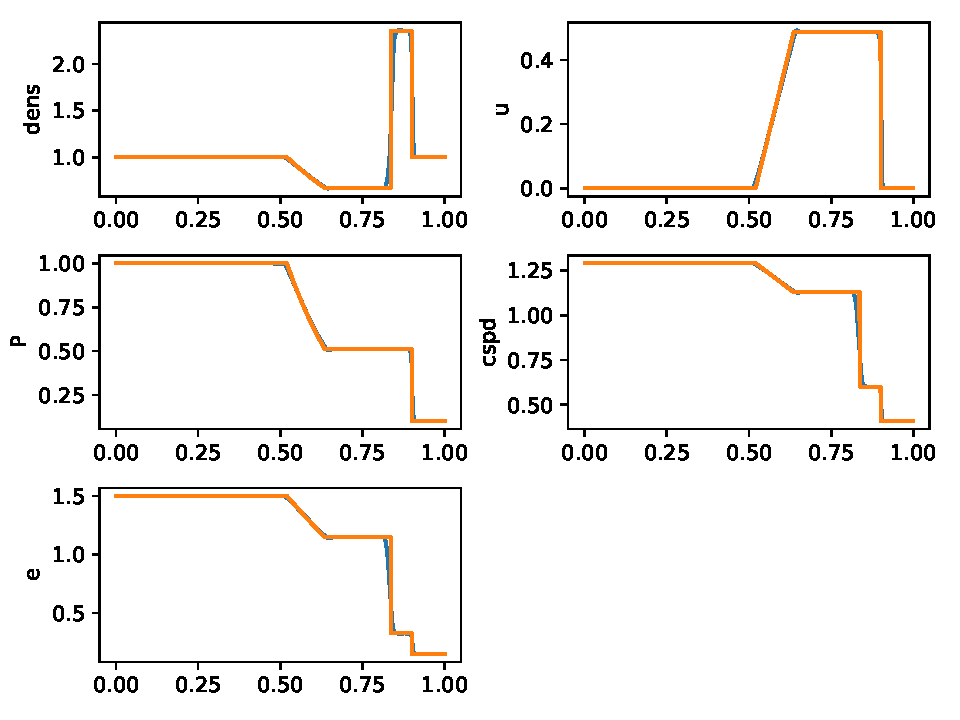
\includegraphics[scale=0.8]{figures/sod1-BC9-PV.pdf}
 \caption{$sod_1$ results for $t = 0.1780$ compared to the exact solution. Flexi data are the blue curves and exact are red.}
 \label{fig:Sod1-1}
\end{figure}

\begin{table}[h!]
 \centering
 \begin{tabular}{|c|c|} \hline
   Variable & $\bar{\epsilon}$ \\ \hline \hline
   $\rho$ & 0.00156 \\
   $v_x$  & 0.00071 \\
   $u$     & 0.00112 \\
   $P$     & 0.00059 \\ \hline
 \end{tabular}
 \caption{Average error for the $Sod_1$ Problem}\label{tab:sod1Eps}
\end{table}


\paragraph{Case $Sod_2$}

In a second case, Sod examined the effects of shock and rarefaction waves reflecting off the walls at $x_L = 0$ and $x_R = 1$ with $x_D = 0.5$ using inflow/outflow boundary conditions.  His results are at $t = 0.2746$. In this case shown in Figure~\ref{fig:Sod2-BC2}, Flexi was run using a mesh generated with HOPR using the input deck listed in \ref{ssec:hoprin-sod2-BC2} and Flexi executed using the input listed in \ref{ssec:flexiin-sod2-BC2}. The flexi results are nearly identical to the exact solution, however it is noted the these results are dramatically different from the results shown in Figure 11 of \cite{sod1}.

\begin{figure}[h!]
 \centering
 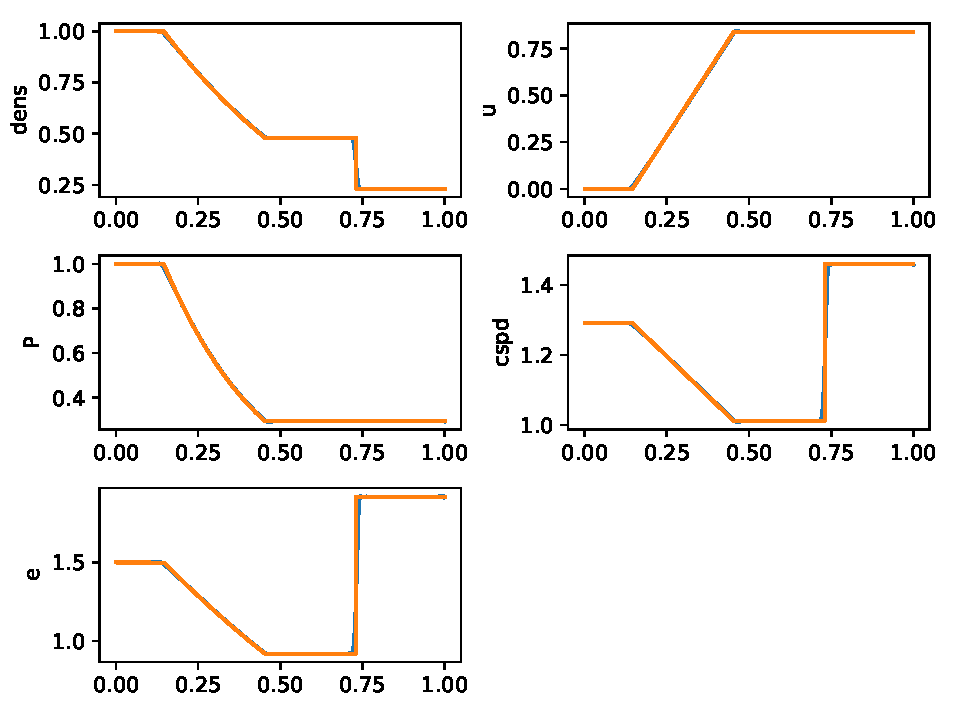
\includegraphics[scale=0.8]{figures/sod2-BC2-PV.pdf}
 \caption{$sod_2$ results for $t = 0.2746$ with inflow/outflow boundary conditions as compared to the exact solution (red curves). Flexi data are in blue.}
 \label{fig:Sod2-BC2}
\end{figure}

If instead of inflow/outflow boundary condition they are changed to symmetry conditions, the flexi results compared with the exact solution are shown in Figure~\ref{fig:Sod2-BC9}.  These results show the effect of the shock reflecting from the $x_R$ boundary. Note that the exact solution has only inflow/outflow boundaries. Flexi was run using a mesh generated with HOPR using the input deck listed in \ref{ssec:hoprin-sod2-BC9} and Flexi executed using the input listed in \ref{ssec:flexiin-sod2-BC9}.

\begin{figure}[h!]
 \centering
 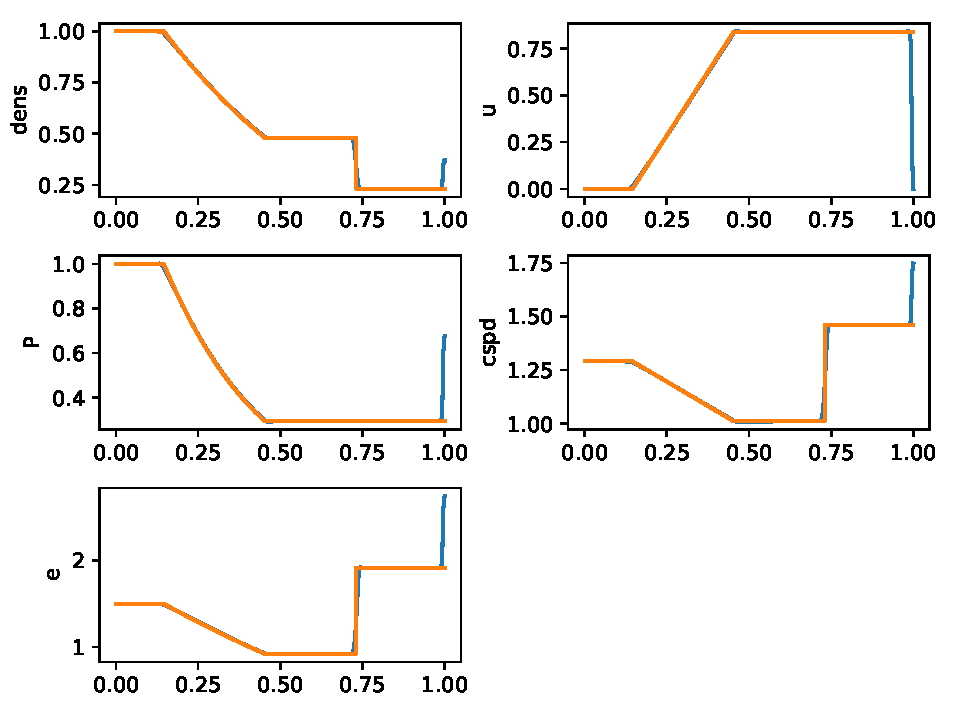
\includegraphics[scale=0.8]{figures/sod2-BC9-PV.pdf}
 \caption{$sod_2$ results for $t = 0.2746$ with symmetry boundary conditions as compared to the exact solution (red curves). Flexi data are blue curves. Note the effect of the symmetry condition at the right boundary in the flexi results and that the exact solution does not have symmetry boundary conditions.}
 \label{fig:Sod2-BC9}
\end{figure}

Table~\ref{tab:sod2Eps} shows the average error for the Flexi solution is less than $0.0015$.

\begin{table}[h!]
 \centering
 \begin{tabular}{|c|c|} \hline
   Variable & $\bar{\epsilon}$ \\ \hline \hline
   $\rho$ & 0.00065 \\
   $v_x$  & 0.00135 \\
   $u$     & 0.00147 \\
   $P$     & 0.00091 \\ \hline
 \end{tabular}
 \caption{Average error for the $Sod_2$ Problem}\label{tab:sod2Eps}
\end{table}

\paragraph{Case $Sod_3$: Symmetry Boundary Conditions}

In a third case (\textit{c.f.:} \ref{tab:sodIC}), Sod examined a challenging Rieman problem in the usual domain $x_L = 0$ and $x_R = 1$ with $x_D = 0.3$ using symmetry boundary conditions.  Here, the Left gas has density $\rho_L = 1.,$ and Right density $\rho_R = 0.001$ and Left pressure $P = 6.6667e^{2}$ and Right pressure $P_R = 6.6667e{-6}$.  This is essentially propagation of an ideal gas into a vacuum.

Flexi was unable to complete these calculations due to NaN's being generated in the time discretization step.  However, attempts were made to run flexi for less extreme initial conditions: $\rho_L = 1.$, $\rho_R = 0.2$ and $P_L = 66.667$, $P_R = 0.066667$. Results are at $t = 0.01812$.  as shown in Figure~\ref{fig:multiSod3-BC9}. Flexi was run using a mesh generated with HOPR using the input deck listed in \ref{ssec:hoprin-sod3-BC9} and Flexi executed using the input listed in \ref{ssec:flexiin-sod3-BC9}.

\begin{figure}[h!]
 \centering
 %\includegraphics[scale=0.8]{figures/sod3-BC9-g-5o3-t-1812o10000-x0-3o10.pdf}
 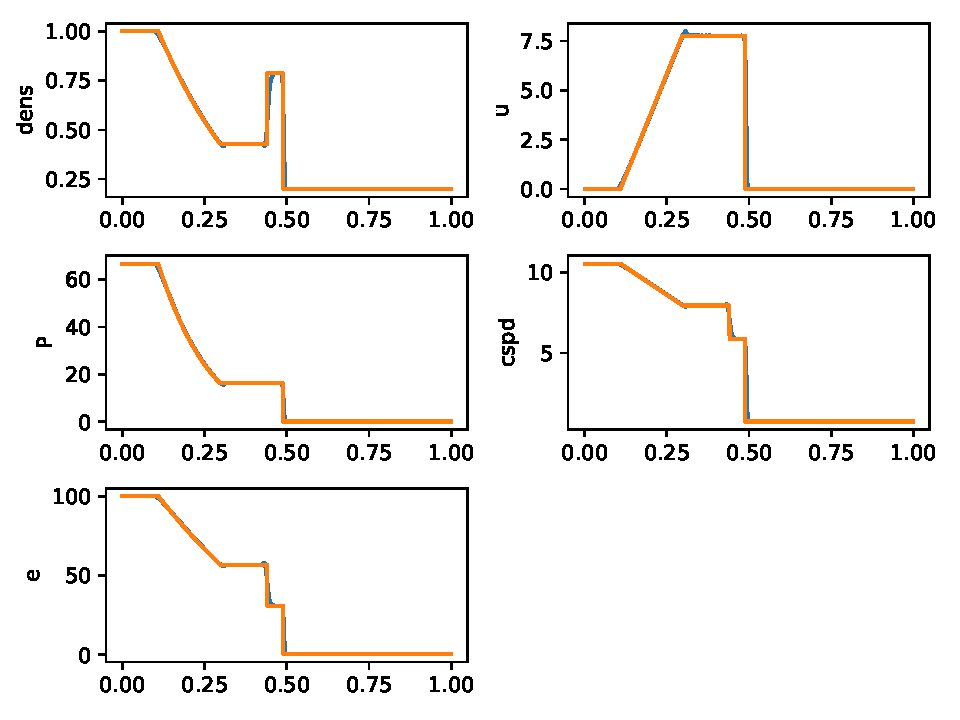
\includegraphics[scale=0.8]{figures/sod3-BC9-PV.pdf}
 \caption{$sod_{3-mod}$ results for the modified input discussed above at $t = 0.01812$ (blue curves) compared to the exact solution (red curves).}
 \label{fig:multiSod3-BC9}
\end{figure}

Table~\ref{tab:sod3Eps} shows the average error for the Flexi solution is less than $0.007$.

\begin{table}[h!]
 \centering
 \begin{tabular}{|c|c|} \hline
   Variable & $\bar{\epsilon}$ \\ \hline \hline
   $\rho$ & 0.00092 \\
   $v_x$  & 0.00330 \\
   $u$     & 0.00712 \\
   $P$     & 0.00425 \\ \hline
 \end{tabular}
 \caption{Average error for the $Sod_{3-mod}$ Problem}\label{tab:sod3Eps}
\end{table}

\paragraph{Conclusions}\label{pp:sodConc}
For the cases presented in this section, Flexi was able to very nearly reproduce the exact solutions. These results ran with the number of Finite Volume zones at 2 to 4\% of the total zones; those zones handling the shock/rarefaction dynamics.



\subsubsection{The Einfeldt Problem}\label{ss:einfeldt}

In 1986  Einfeldt, \textit{et al.}~\cite{einfeldt}  studied Riemann problems using Godunov's method near low densities. Referring to Figure~\ref{fig:shockTube} the domain  $[x |  -0.5 \le x \le 0.5]$ has  a diaphragm at $x = 0.$ and is filled with ideal gases with $\gamma = 1.4$, density $\rho = 1$, and total energy per unit volume $E = 3$ on both sides, but with x-momentum on the left $m_{l_1} = -2$ and on the right $m_{r_1} = 2$ (with $m_{r_{23}} = m_{l_{23}} = 0$) , creating, as time passes, a region of very low density near the diaphragm.  This is sometimes refered to as the \textit{1,2,3-problem} since the initial state has $[\rho, |m_i|, E] = [1, 2, 3].$ The input decks for hopr and flexi are listed in the \ref{ssec:hoprin-einfeldt} and \ref{ssec:flexiin-einfeldt}.  The results at $t = 0.05$ for primitive variables are shown in Figure~\ref{fig:PVmulti123} and for conserved variables in Figure~\ref{fig:multi123}

\begin{table}[h!]
 \begin{center}
  \caption{Initial conditions for Einfeldt's test case.}
  \label{tab:einfeldtIC}
  \begin{tabular}{|c|ccc|cccc|cccc|} \hline
   \textbf{Case} & \multicolumn{3}{c|}{\textbf{Domain}} & \multicolumn{4}{c|}{\textbf{Left Gas}} & \multicolumn{4}{c|}{\textbf{Right Gas}} \\ \hline
   \multirow{2}{*}{$123$} & $x_L$ & $x_D$ & $x_R$ & $\rho$ & $u$ & $P$ & $\gamma$ & $\rho$ & $u$ & $P$ & $\gamma$ \\ \cline{2-12}
   \multicolumn{1}{|c|}{} & 0. & 0.5 & 1.  & 1. & -2. & 0.4 & 1.4 & 1. & 2. & 0.4 & 1.4 \\ \hline
  \end{tabular}
 \end{center}
\end{table}

\begin{figure}[h!]
 \centering
 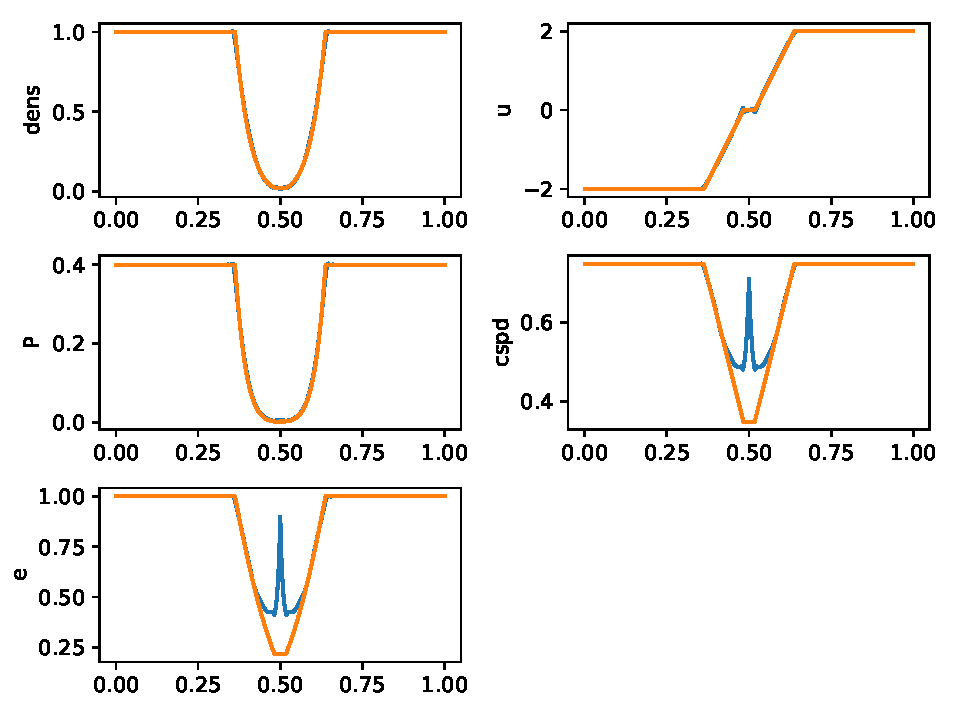
\includegraphics[scale=0.8]{figures/einfeldt-PV.pdf}
 \caption{Einfeldt problem at $t = 0.05$ with 100 equal sized elements in the $x$-direction, but showing the conserved density and the primitive variables: specific internal energy, x-velocity, pressure, and sound speed.  These data reflect the slight oscillation of the very low density region near the diaphragm. Each of these primitive variables are computed using density as a divisor causing large deviations in those variables. Exact data are the blue curves.}
 \label{fig:PVmulti123}
\end{figure}

\begin{figure}[h!]
 \centering
 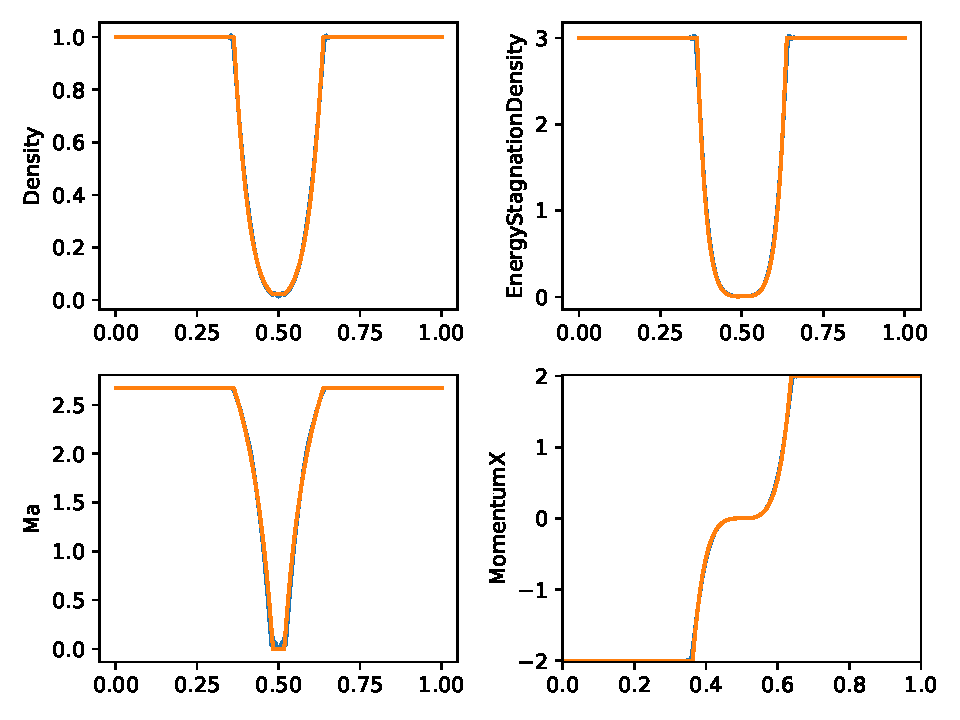
\includegraphics[scale=0.8]{figures/einfeldt-CV.pdf}
 \caption{Einfeldt problem at $t = 0.05$ with 100 equal sized elements in the $x$-direction; showing conserved Flexi variables (blue curves) compared to the exact solution (red curves).}
 \label{fig:multi123}
\end{figure}


Tables~\ref{tab:123Eps} shows the average error for the Flexi solution is less than $0.0016$ with conserved variables being much closer to the exact solution.

\begin{table}[h!]
 \centering
 \begin{tabular}{|c|c|} \hline
   Variable & $\bar{\epsilon}$ \\ \hline \hline
   $\rho$ & 4.7E-4 \\
   $m_x$  & 7.2E-4 \\
   $E$      & 9.3E-4 \\ \hline
   $v_x$  & 6.4E-4 \\
   $u$     & 1.59E-3 \\
   $P$     & 3.2E-4 \\ \hline
 \end{tabular}
 \caption{Average error (\textit{c.f.,} Eq.~\ref{eq:error}) for the Einfeldt Problem}\label{tab:123Eps}
\end{table}

\paragraph{Conclusions}
Flexi results for the Einfeldt problem match very well with the exact solution for conserved variables, although the density near the diaphragm shows oscillations. Any derived variable having density will reflect large discrepancies in that region due to division by very small numbers.


\subsubsection{The LeBlanc Problem}\label{ss:leblanc}

The third shock tube problem is the LeBlanc\footnote{Attempts to find the original citation for this test problem were unsuccessful until William Rider of Sandia NationalLaboratory provided the following information: ``I believe it was called TP37 in the JOWOG 42 structure at the Labs.  The first mention of it in the literature I can find is a AIAA paper by Pember and Anderson (LLNL) \cite{Pember} in 2001.  They also did a longer report comparing methods in 2000 (comparing Eulerian methods to ALE methods with LeBlanc being one of the problems).  They point to a paper by Benson \cite{Benson} as a source along with personal communications with Jim LeBlanc.''} problem.  The setup for this problem is again illustrated in Figure~\ref{fig:shockTube} with initial data  given in Table~\ref{tab:leblancIC}. This is an extreme test problem due to the very small density ratio of $10^{-3}$ and pressure ratio of $10^{-9}$.  The parameter input files for Flexi is in \ref{ssec:flexiin-leblanc} and for hopr \ref{ssec:hoprin-leblanc}. Results are show for $t = 6.$ in Figure~\ref{fig:CVleblanc} for conserved variables while primitive variables are shown in Figure~\ref{fig:PVleblanc}.

\begin{table}[h!]
 \begin{center}
  \caption{Initial conditions for LeBlanc's test case.}
  \label{tab:leblancIC}
  \begin{tabular}{|c|ccc|cccc|cccc|} \hline
   \textbf{Case} & \multicolumn{3}{c|}{\textbf{Domain}} & \multicolumn{4}{c|}{\textbf{Left Gas}} & \multicolumn{4}{c|}{\textbf{Right Gas}} \\ \hline
   \multirow{2}{*}{$1$} & $x_L$ & $x_D$ & $x_R$ & $\rho$ & $u$ & $P$ & $\gamma$ & $\rho$ & $u$ & $P$ & $\gamma$ \\ \cline{2-12}
   \multicolumn{1}{|c|}{} & 0. & 3. & 9.  & 1. & 0. & 2/3 E-1 & 5/3 & 1.E-3 & 0. & 2/3 E-10 & 5/3 \\ \hline
  \end{tabular}
 \end{center}
\end{table}

\begin{figure}[h!]
 \centering
 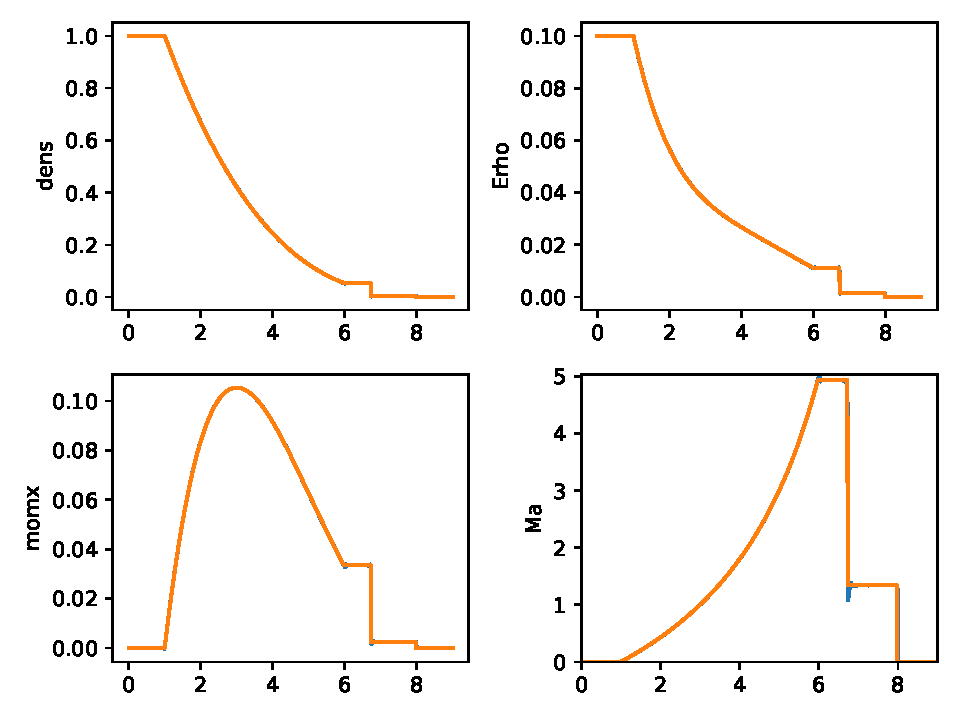
\includegraphics[scale=0.8]{figures/leblanc-CV.pdf}
 \caption{LeBlanc problem at $t = 6.$ with 100 equal sized elements in the $x$-direction showing the conserved variables.  Comparison is made to the exact solution (in red.)  The derived Mach number shows slight variation from the exact solution at the shock front, but the conserved variables are nearly identical to it.}
 \label{fig:CVleblanc}
\end{figure}

\begin{figure}[h!]
 \centering
 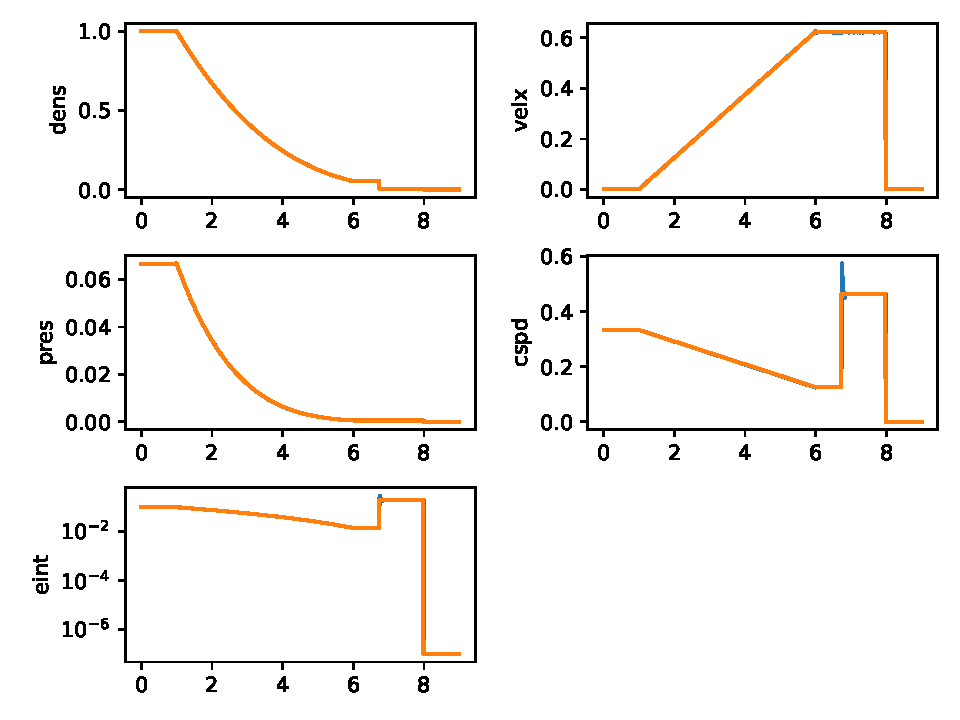
\includegraphics[scale=0.8]{figures/leblanc-PV.pdf}
 \caption{LeBlanc problem at $t = 6.$ with 100 equal sized elements in the $x$-direction showing primitive variables.  Comparison is made to the exact solution (in red.)}
 \label{fig:PVleblanc}
\end{figure}
\noindent Table~\ref{tab:leblancEps} shows the average error in the Flexi solution to be less than $9.04E-4$.

\begin{table}[h!]
 \centering
 \begin{tabular}{|c|c|} \hline
   Variable & $\bar{\epsilon}$ \\ \hline \hline
   $\rho$ & 1.41E-4 \\
   $m_x$  & 1.11E-4 \\
   $E$      & 6.47E-5 \\ \hline
   $v_x$  & 9.04E-4 \\
   $u$     & 5.76E-4 \\
   $P$     & 2.67E-5 \\ \hline
 \end{tabular}
 \caption{Average error (\textit{c.f.,} Eq.~\ref{eq:error}) for the LeBlanc Problem}\label{tab:leblancEps}
\end{table}

\paragraph{Conclusions}

Flexi performs very well on the LeBlanc problem with only minor overshoot at the shock front.


\section{Two-Dimensional Results}\label{sec:2D}

Two cases of two-dimensional Riemann problems were executed using Flexi compiled using the configuration file in \ref{ssec:2Dconfig}.

\subsection{The Sedov Problem}\label{ss:sedov}

The dynamic problem of propagation of a blast wave in a $\gamma$-law compressible gas has been the focus of many researchers and has come to be known as the Sedov Problem.  The large bibliography of Sedov-studies may be summarized as in Griffiths (Chapter 10, Case Study: Taylor-Sedov Blast Wave) \cite{Griffiths} or Kamm and Timmes \cite{Kamm} and dates from the early work of Taylor \cite{Taylor} and von Neumann \cite{vonN} in 1941,  L.\  I.\  Sedov \cite{Sedov46} in 1946 (and 1959 \cite{Sedov}).

The results shown here are as defined in the last paragraph of Section 4.1 of Kamm and Timmes~ \cite{Kamm} for the geometry shown in Figure~\ref{fig:SedovGeom}.  Here, $H = 2 W$, $W = 1.25 \  \mathrm{cm}$, $D= 0.025 \ \mathrm{cm}$.  The mesh is constructed from hexahedra having  $\Delta x = \Delta y = \Delta z = W/50 = 0.025$ cm so that the mesh has 50 elements in the $X(1)$ direction, 100 in the $X(2)$ direction and 1 in the $X(3)$ direction.  Although the simulation is executed in a Cartesian system and because of the initial conditions being independent of $X(3)$, the problem becomes a two-dimensional Cylindrical geometry simulation.  Kamm and Timmes propose that for this case the stationary gas has $\gamma = 1.4$ and that at $t = 0$, the density is uniform at $\rho = 1$ gm/cc and that the blast total energy per unit depth is  $E_0 = 0.311357$ erg.  This value is such that at $t = 1\ s$ the blast wave will have a radius of $0.75$ cm.  Flexi requires initial values for density, momentum (x, y, z values) and pressure.  Consequently, since $ P = (\gamma - 1) \rho u$ and that initially with zero kinetic energy of the gas then $E_0/V_0 = \rho u$ and $V_0 = \pi R^2 Z$, where $Z$ is unit depth.  Then

\begin{eqnarray}
P_0 & = & (\gamma - 1) \frac{E_0 Z}{V_0} \\
   & = & (\gamma -1) \frac{E_0}{\pi R^2}  \nonumber \\
    & = & \frac{0.4 \ 0.311357}{ \pi\  0.025^2} \ \mathrm{dynes}/\mathrm{cm}^2 \nonumber \\
    & = & 63.43 \ \mathrm{dynes}/\mathrm{cm}^2 \nonumber
\end{eqnarray}
\noindent Outside of the blast zone, the intial pressure is set to $1. E -8$.

\begin{figure}[h!]
 \begin{center}
  \input{figures/Sedov-geom.pdf_t}
  \caption{The two-dimensional cylindrical Sedov problem geometry and mesh setup.}
  \label{fig:SedovGeom}
 \end{center}
\end{figure}

The two-dimensional initial pressure and final density ($t = 1.\ s$) fields are shown in Figure~\ref{fig:sedov2D} and for comparison to exact results the extracted line plots for this simulation are presented in Figures~\ref{fig:CVsedov} and \ref{fig:PVsedov}.  The line plots are along a $45^o$ ray from the origin into the first quardant.  Flexi mesh and input files are listed in \ref{ssec:hoprin-sedov} and \ref{ssec:flexiin-sedov}.  In the Flexi input file, note that the value of $\mathrm{IniExactFunc} = 1342$ and $\mathrm{eradius\_in} = 0.025$.  This is a special exact function coded into flexi/src/equations/navierstokes/idealgas/exactfunc.f90 which specifies that if $X(1)^2 + X(2)^2 \ge \mathrm{eradius}$\_$\mathrm{in}^2$ for all $X(3)$ then RefState 1 applies, otherwise RefState 2 applies.  The Flexi results were extracted from ParaView at $t = 1.\ s$ using the plotOverLine app, with the line running from $(0,0,-0.0125)$ to $(1.25, 1.25, -0.0125)$.

\begin{figure}[h!]
\centering
\begin{subfigure}[h!]{0.9\linewidth}
\centering
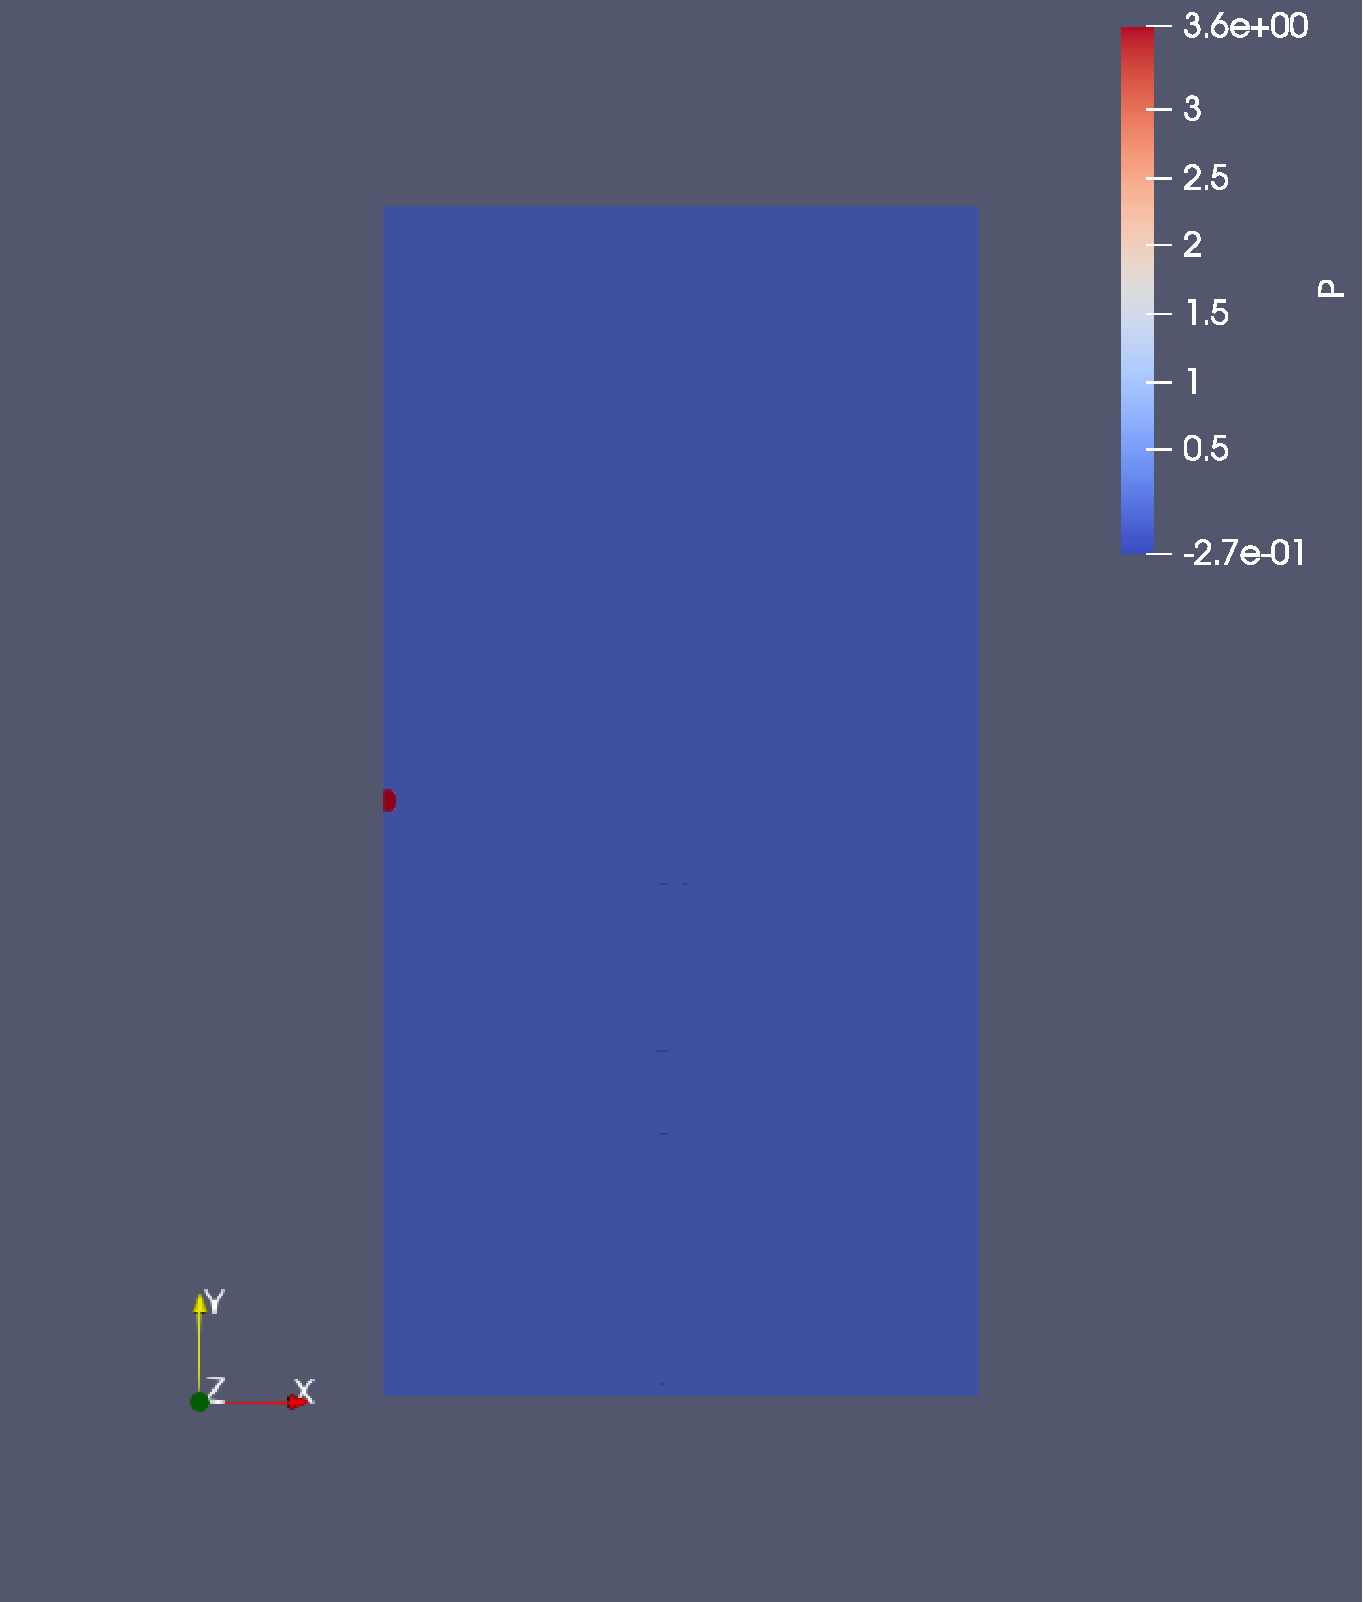
\includegraphics[scale=0.25]{figures/sedov-00-P.pdf }
\caption{Initial pressure field for the Sedov problem showing the small (2 element) region of initially high pressure.\bigskip \bigskip}
  \label{fig:sedov-0}
\end{subfigure}

\begin{subfigure}[h!]{0.9\linewidth}
\centering
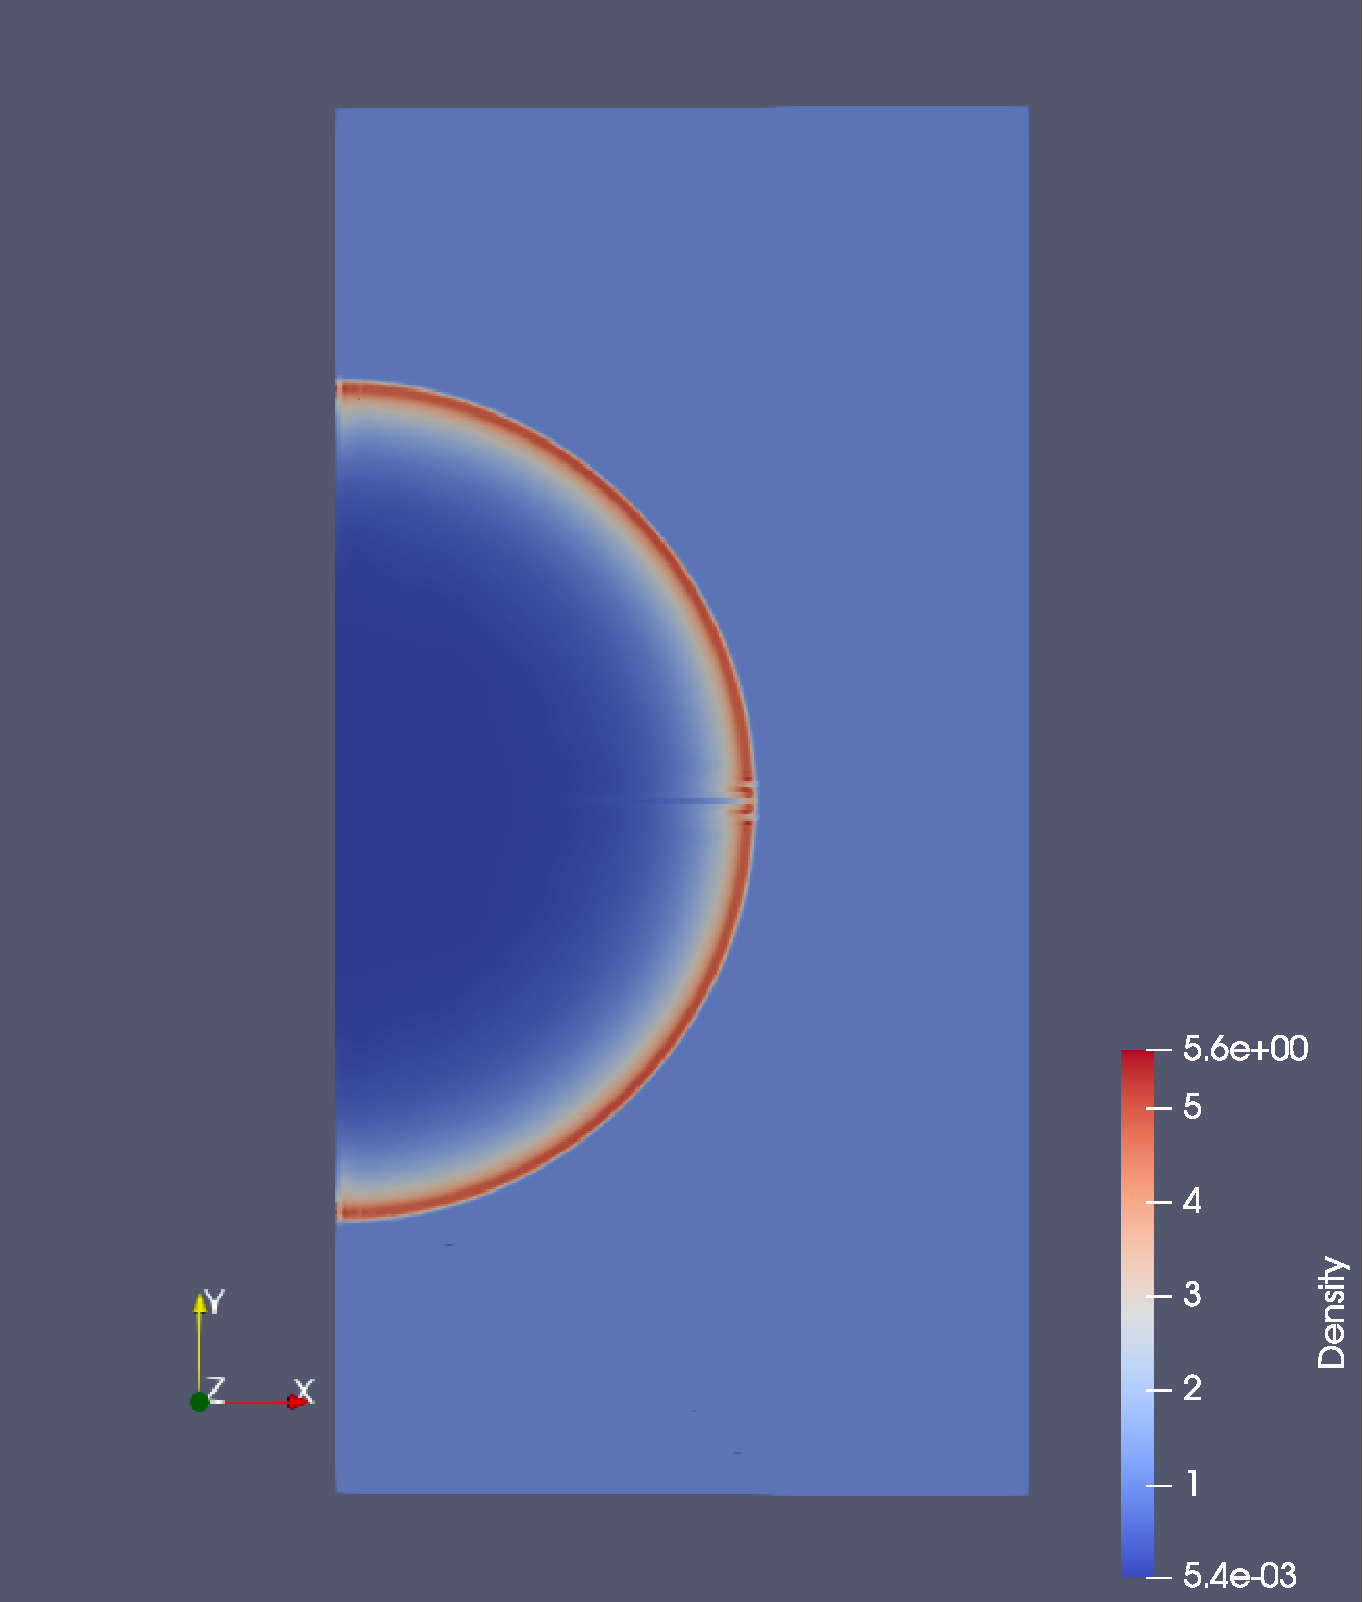
\includegraphics[scale=0.25]{figures/sedov-10-den.pdf }
\caption{Final $t = 1. \  s$ density field for the Sedov problem. Some minor irregularities are shown at the shock front along both the x and y-axes. However the shock front arrives at a radius very close to $R = 0.75$ as expected.}
  \label{fig:sedov-10}
\end{subfigure}
\caption{The Sedov problem results for the density field.}
\label{fig:sedov2D}
\end{figure}

\begin{figure}[h!]
 \centering
 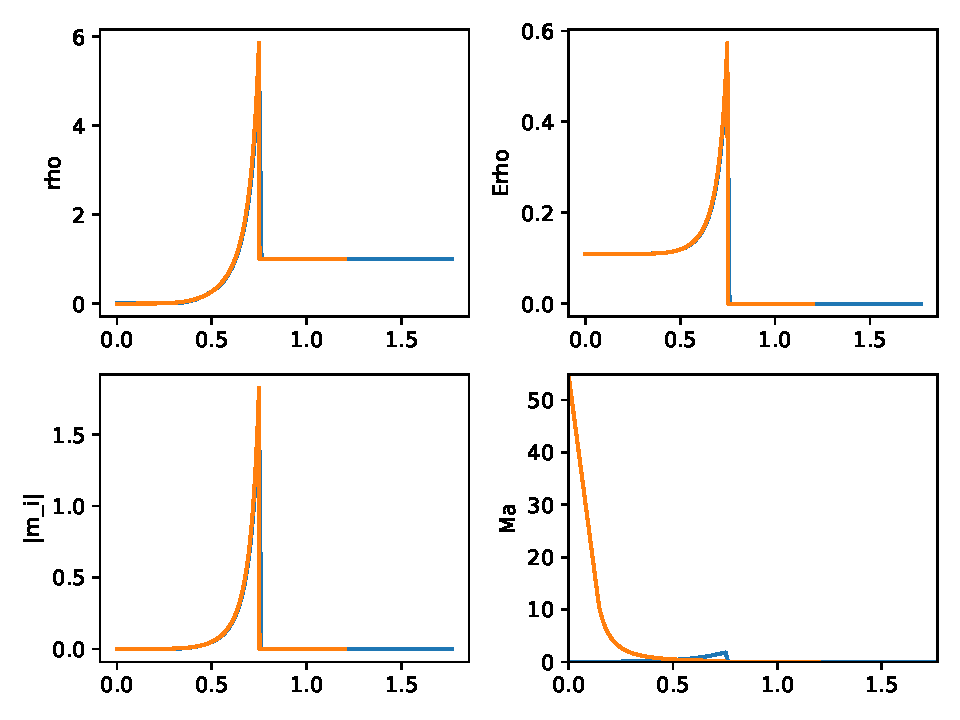
\includegraphics[scale=0.8]{figures/sedov-CV.pdf}
 \caption{Sedov problem at $t = 1.\ s$ and showing the conserved variables.  Comparison is made to the exact solution (in blue.) }
 \label{fig:CVsedov}
\end{figure}

\begin{figure}[h!]
 \centering
 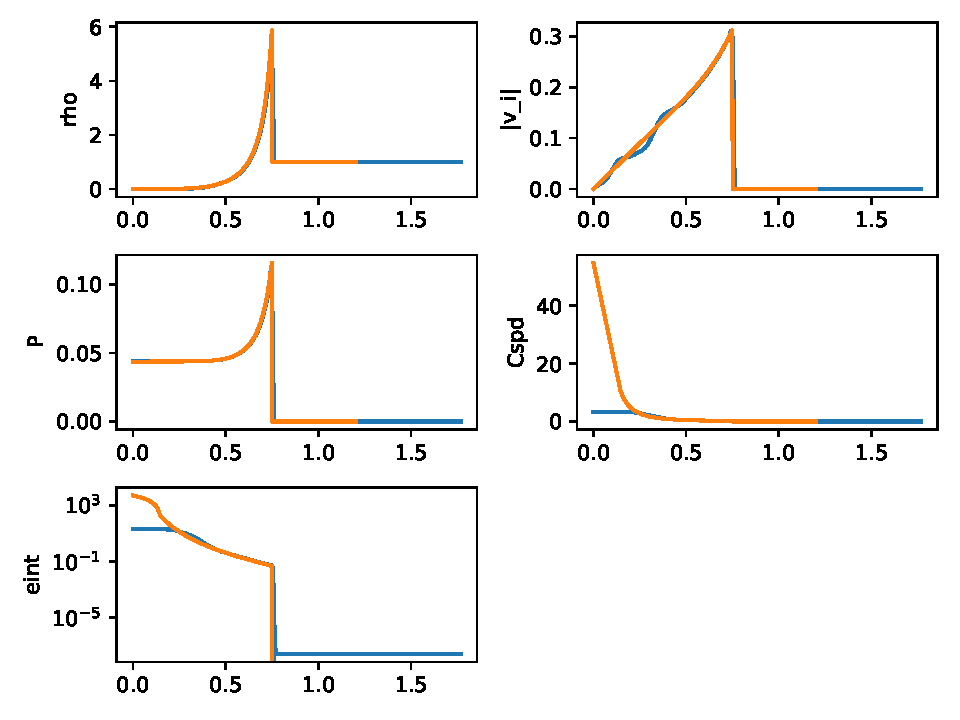
\includegraphics[scale=0.8]{figures/sedov-PV.pdf}
 \caption{Sedov problem at $t = 1. \ s$, showing primitive variables.  Comparison is made to the exact solution (in blue.)}
 \label{fig:PVsedov}
\end{figure}

\noindent It is noted that the shock arrives very close to a radius of $0.75$ at $t = 1.\ s$  Table~\ref{tab:sedovEps} shows the average error in the Flexi solution to be less than $5.7E-3$ except for specific internal energy.

\begin{table}[h!]
 \centering
 \begin{tabular}{|c|c|} \hline
   Variable & $\bar{\epsilon}$ \\ \hline \hline
   $\rho$ & 5.62E-3\\
   $|m_i|$  & 3.33E-3 \\
   $E$      & 1.97 E-3 \\ \hline
   $|v_i|$  & 1.8988E-3 \\
   $u$     & 1.86E-1 \\
   $P$     & 9.86865E-4 \\ \hline
 \end{tabular}
 \caption{Average error (\textit{c.f.,} Eq.~\ref{eq:error}) for the Sedov Problem}\label{tab:sedovEps}
\end{table}

The exact solutions presented for the Sedov Problem were computed using the Sedov solver in ExactPack \cite{exactpack}, a newly released Python3 package designed specfically to be used as code verification.  It is available from \url{https://github.com/lanl/ExactPack}.  The Doebling Sedov solver was modified to compute conserved variables and to print out exact solution data files.

\paragraph{Conclusions}
These results show a very good agreement between Flexi and exact results for this challenging two-dimensional problem.



\subsection{The Hui Problem}\label{ss:hui}

The Implosion problem described in Section 4.7 of  Liska and Wendroff \cite{Liska} was first used by Hui, Li, and Li \cite{Hui} and also, with variants, by Chang, Wang, and Chow \cite{Chang} as a two-dimensional test problem for the Euler equations.  The geometry of the problem is shown in Figure \ref{fig:HuiGeom} where a square box is filled with a gas having $\gamma = 7/5$ and has a diaphragm along the line from point $a$ to point $b$, both of which are a distance $h$ from the origin as shown.  In the cases presented here, $S = 0.3$, $h = 0.15$ with either $\beta = 0 \ \mathrm{rad.}$ or $0.4\ \mathrm{rad.}$  The mesh is rotated as a check of the independance of mesh orientation on the results in Flexi.  In \ref{ssec:hoprin-hui-Rot0} the ``hopr'' mesh input file for the $400 \times 400 \times 1$ element unrotated hexahedral mesh is given while that for the rotated mesh is in \ref{ssec:hoprin-hui-Rot}.

\begin{figure}[h!]
 \begin{center}
  \input{figures/HuiGeometry.pdf_t}
  \caption{The two-dimensional Hui implosion problem geometry.  Points $a$ and $b$ lie on the sides of a square box each a distance $h$ from the origin. The box sides are $S$ in length and is rotated about the origin by an angle $\beta = \frac{\pi}{2} - \alpha$. The line $\overline{ab} = [\sin(\beta) - \cos(\beta)] y - [\sin(\beta) + \cos(\beta)] x + h = 0$.}
  \label{fig:HuiGeom}
 \end{center}
\end{figure}

\subsubsection{Non-rotated Mesh Results}\label{sssec:huiNR}

In \ref{ssec:flexiin-hui-Rot0} the Flexi input data file is given for the unrotated mesh.  It is noted that in those files, the $\mathrm{IniExactFunc}  = 1346$ value was added to the exactfunc.f90 source code so that the Hui problem initial conditions could be applied to the mesh using the additional input variable: $\mathrm{Hui\_Data} = (/\beta, h/)$ (rotation angle in radians, interface distance along box side).  If $X(1) + X(2) > h$, then use $\mathrm{RefState} = (1.0, 0., 0., 0.,  1. )$ (density, x vel, y vel, z vel, pressure), otherwise use $\mathrm{RefState} = (0.125, 0., 0., 0., 0.14 )$ in the low energy region. In addition, the new variable $\mathrm{IndSym} = 1$ is used to switch on a modification to the Persson indicator (in flexi/src/indicator/indicator.f90) assuring that it is symmetric for this problem.

Results for the Hui problem are shown in Fgure~\ref{fig:hui-Rot0} for the initial state (Fig. \ref{fig:hui-Rot0-0}) as well as for $t = 0.05$ and $t = 2.5$.  The early time results (Fig.~\ref{fig:hui-Rot0-005}) compare favorably with Fig.\ 4.10 (especially for WENO and CLAW methods) of Liska and Wendroff \cite{Liska}.  The late time results in Fig.~\ref{fig:hui-Rot0-250} compare favorably with the results of Liska and Wendroff in their Fig.\ 4.11.  That reference (\cite{Liska}) also has links to various animations which are very informative.

\begin{figure}[h!]
\centering
\begin{subfigure}[h!]{0.4\linewidth}
\centering
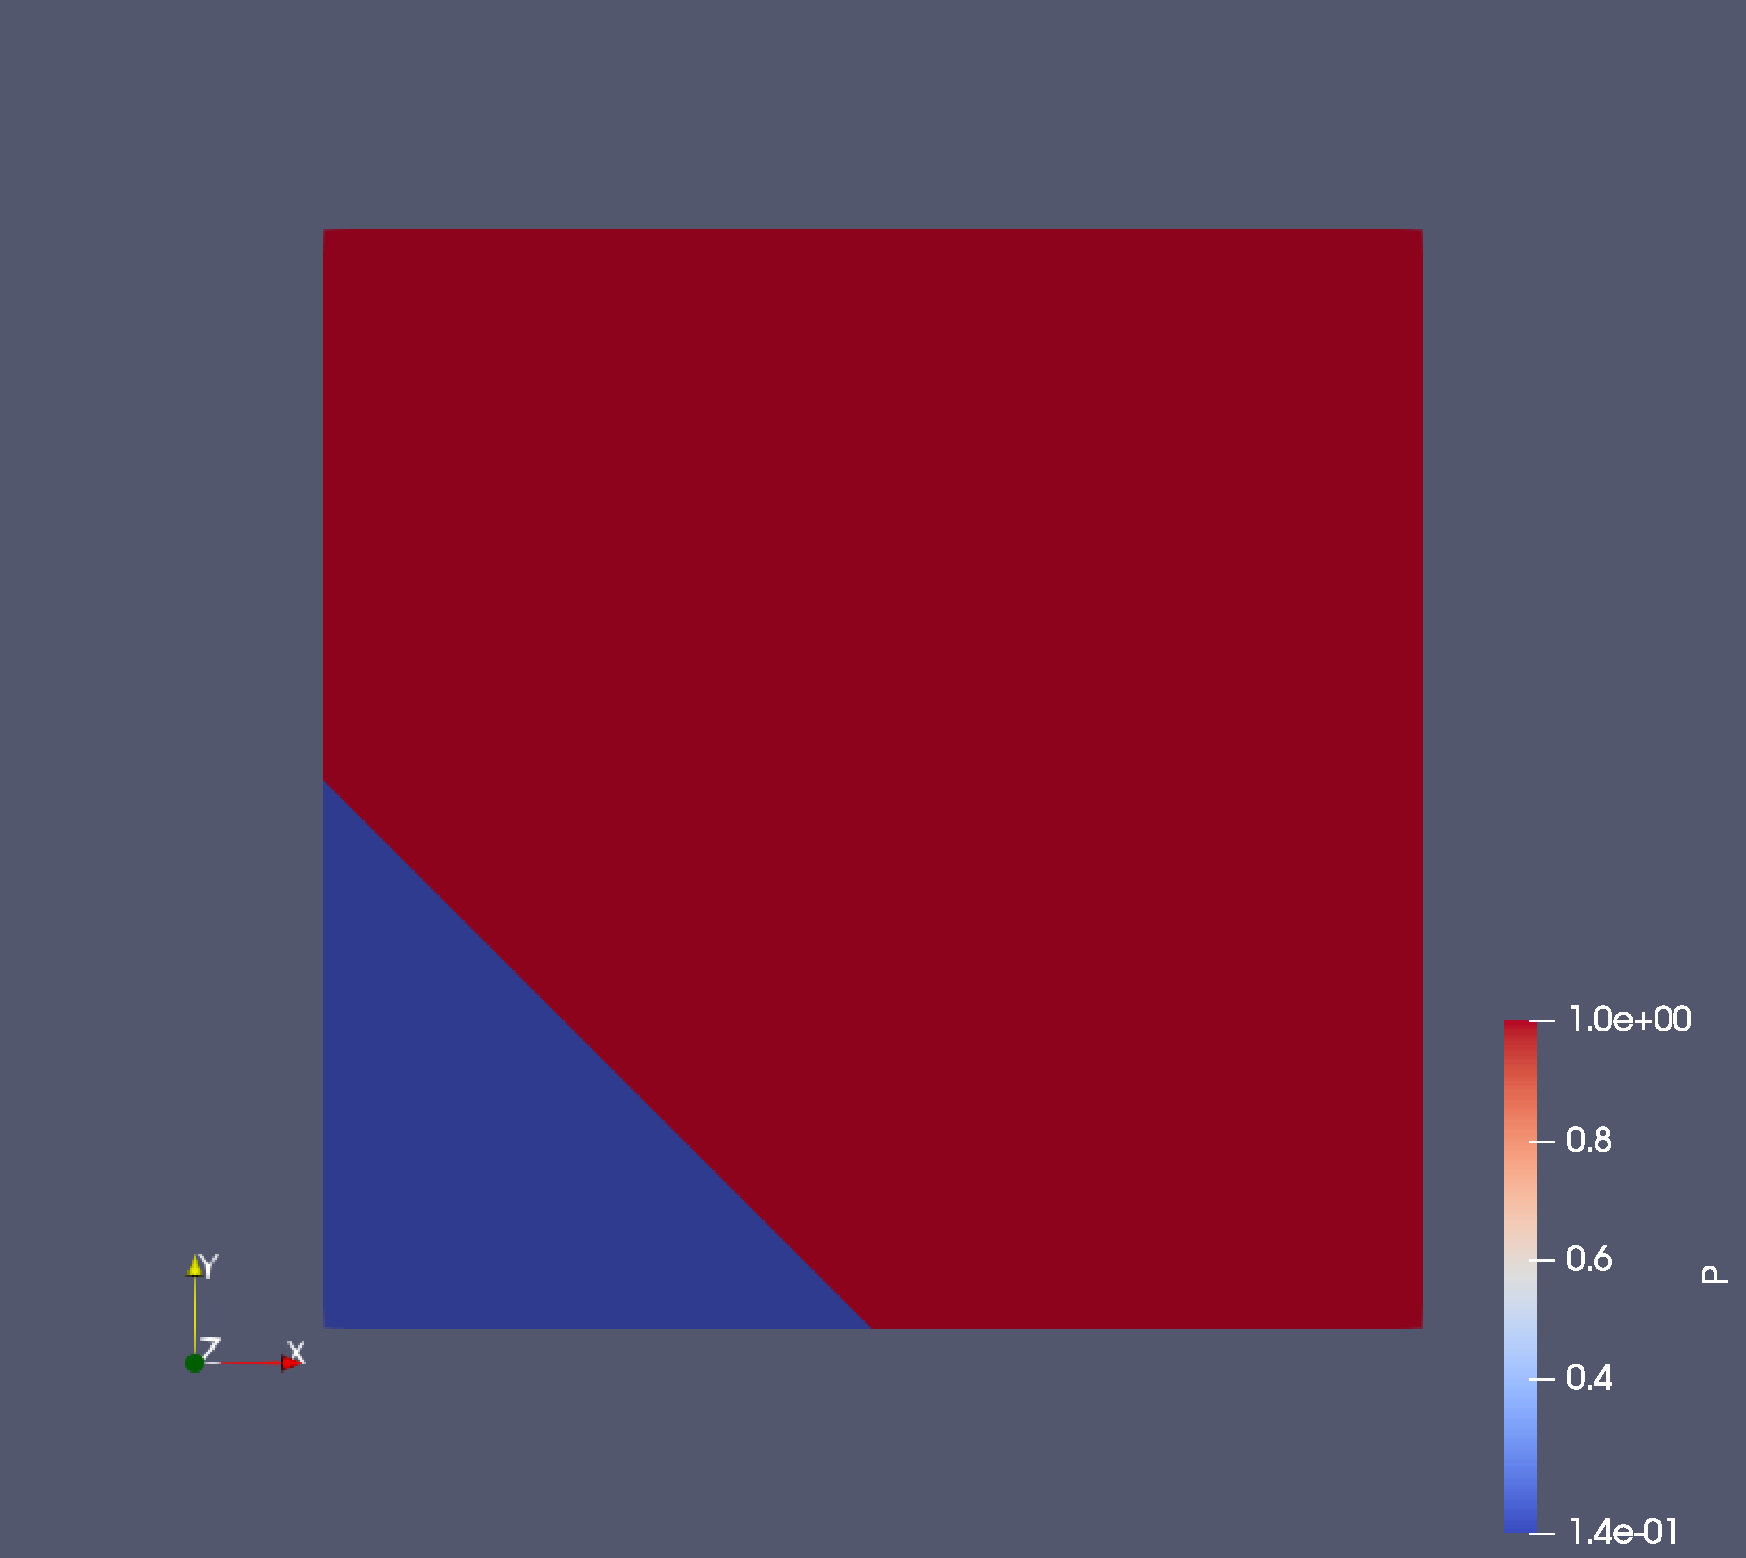
\includegraphics[scale=0.16]{figures/GAH-Hui-400-000.pdf }
\caption{Initial pressure field for the $\beta = 0.$ Hui problem.\bigskip \bigskip}
  \label{fig:hui-Rot0-0}
\end{subfigure}
\begin{subfigure}[h!]{0.4\linewidth}
\centering
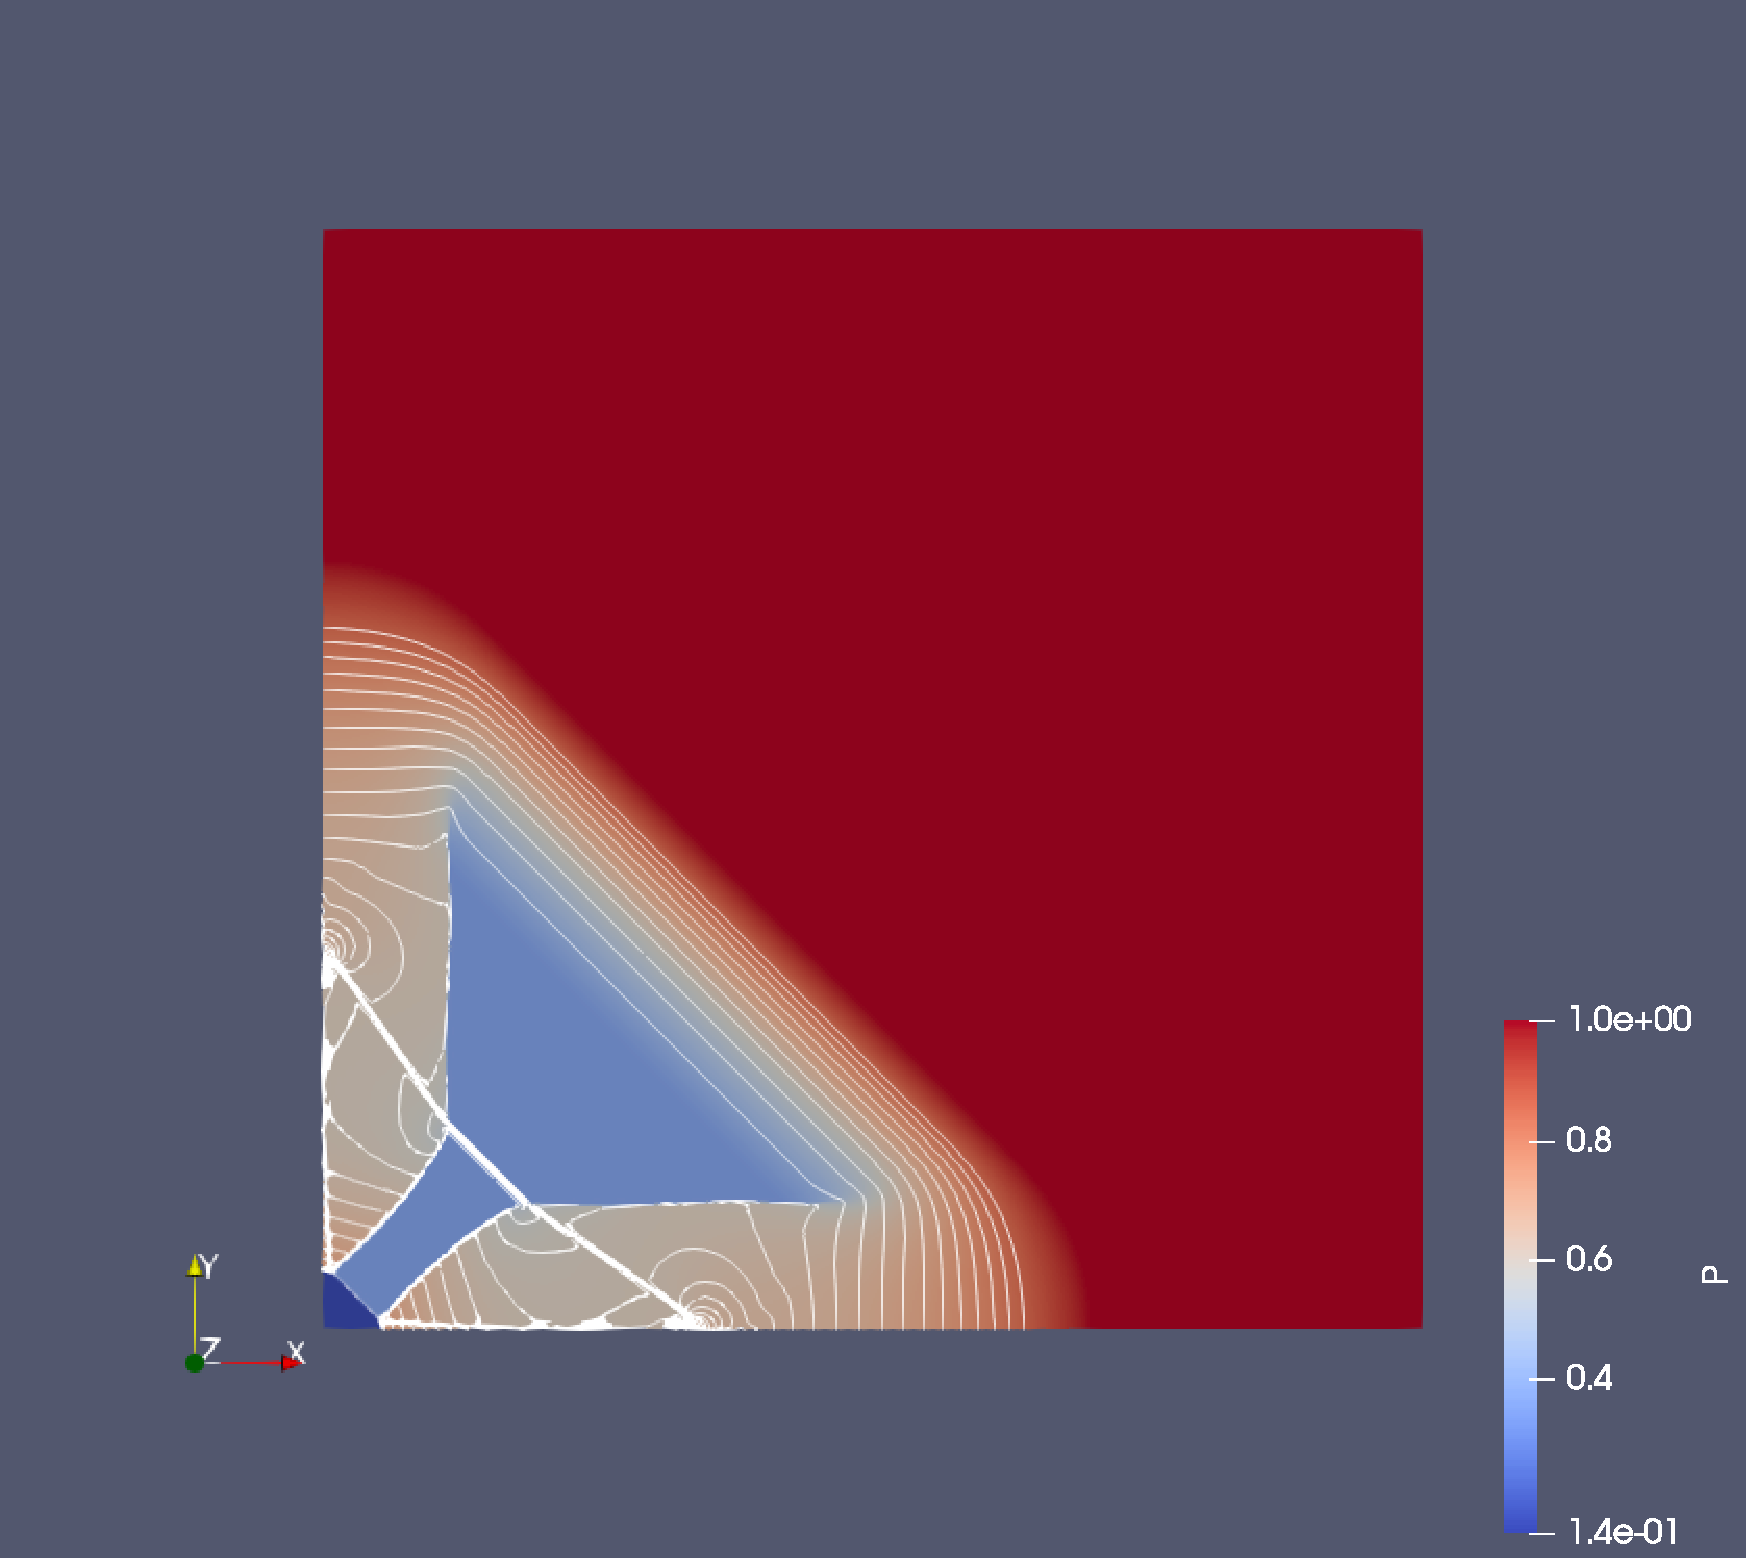
\includegraphics[scale=0.16]{figures/GAH-Hui-400-005.pdf }
\caption{Early time ($t = 0.05$) pressure-density results for the $\beta = 0.$ Hui problem. Density contours show values of $\rho$ in $36$ intervals from $0.125$ to $1.0$.}
  \label{fig:hui-Rot0-005}
\end{subfigure}

\bigskip

\begin{subfigure}[h!]{0.4\linewidth}
\centering
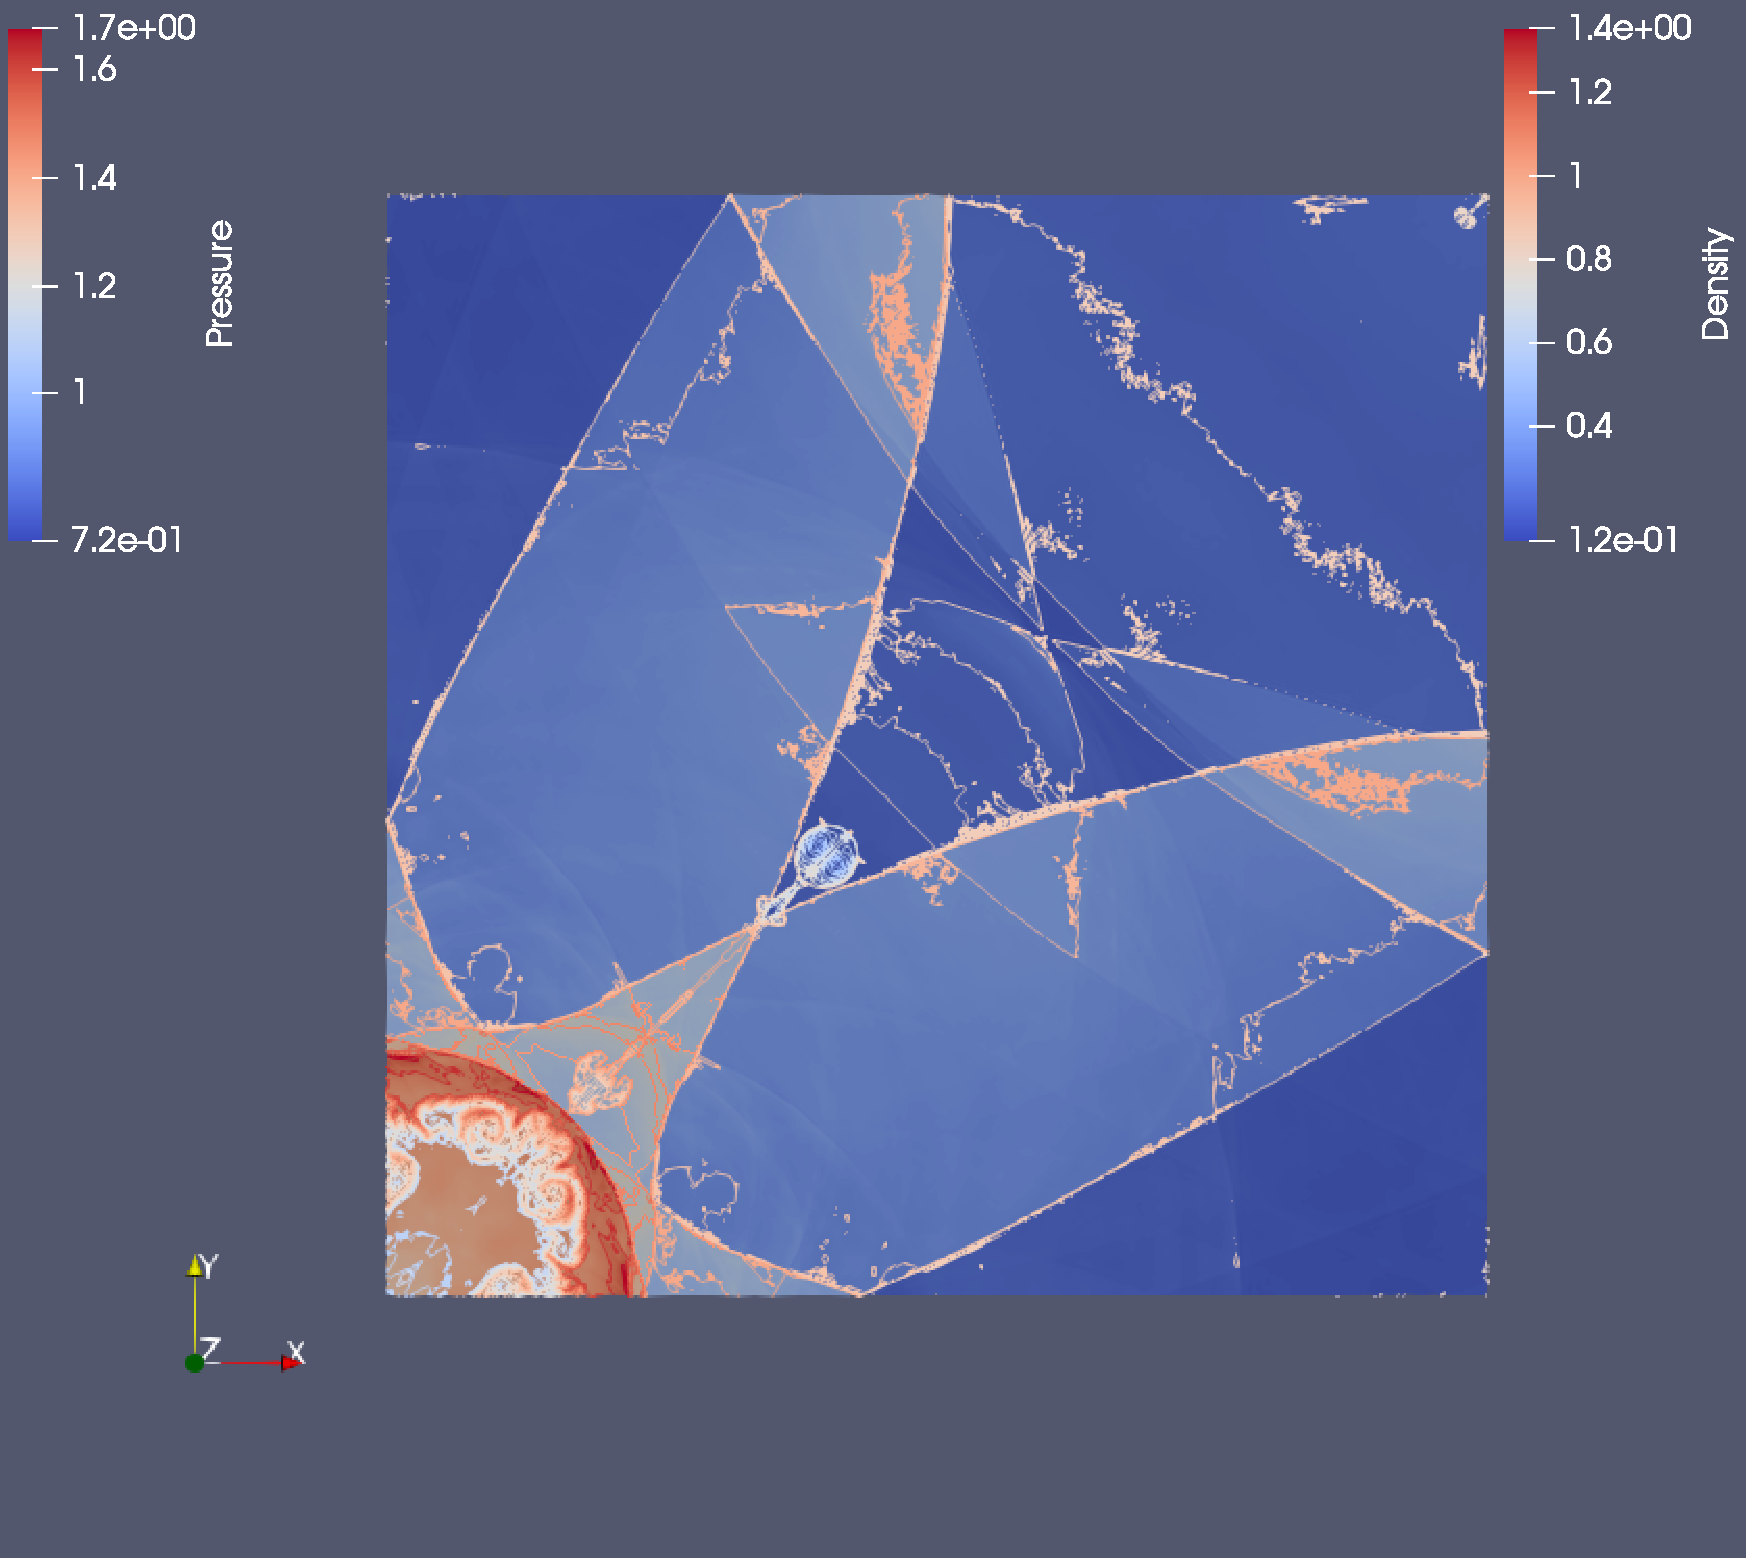
\includegraphics[scale=0.16]{figures/GAH-Hui-400-125.pdf }
\caption{The $t = 1.25$ pressure-density results for the $\beta = 0.$ Hui problem. Density contours show values of $\rho$ in $31$ intervals from $0.35$ to $1.1$.}
  \label{fig:hui-Rot0-125}
\end{subfigure}
\begin{subfigure}[h!]{0.4\linewidth}
\centering
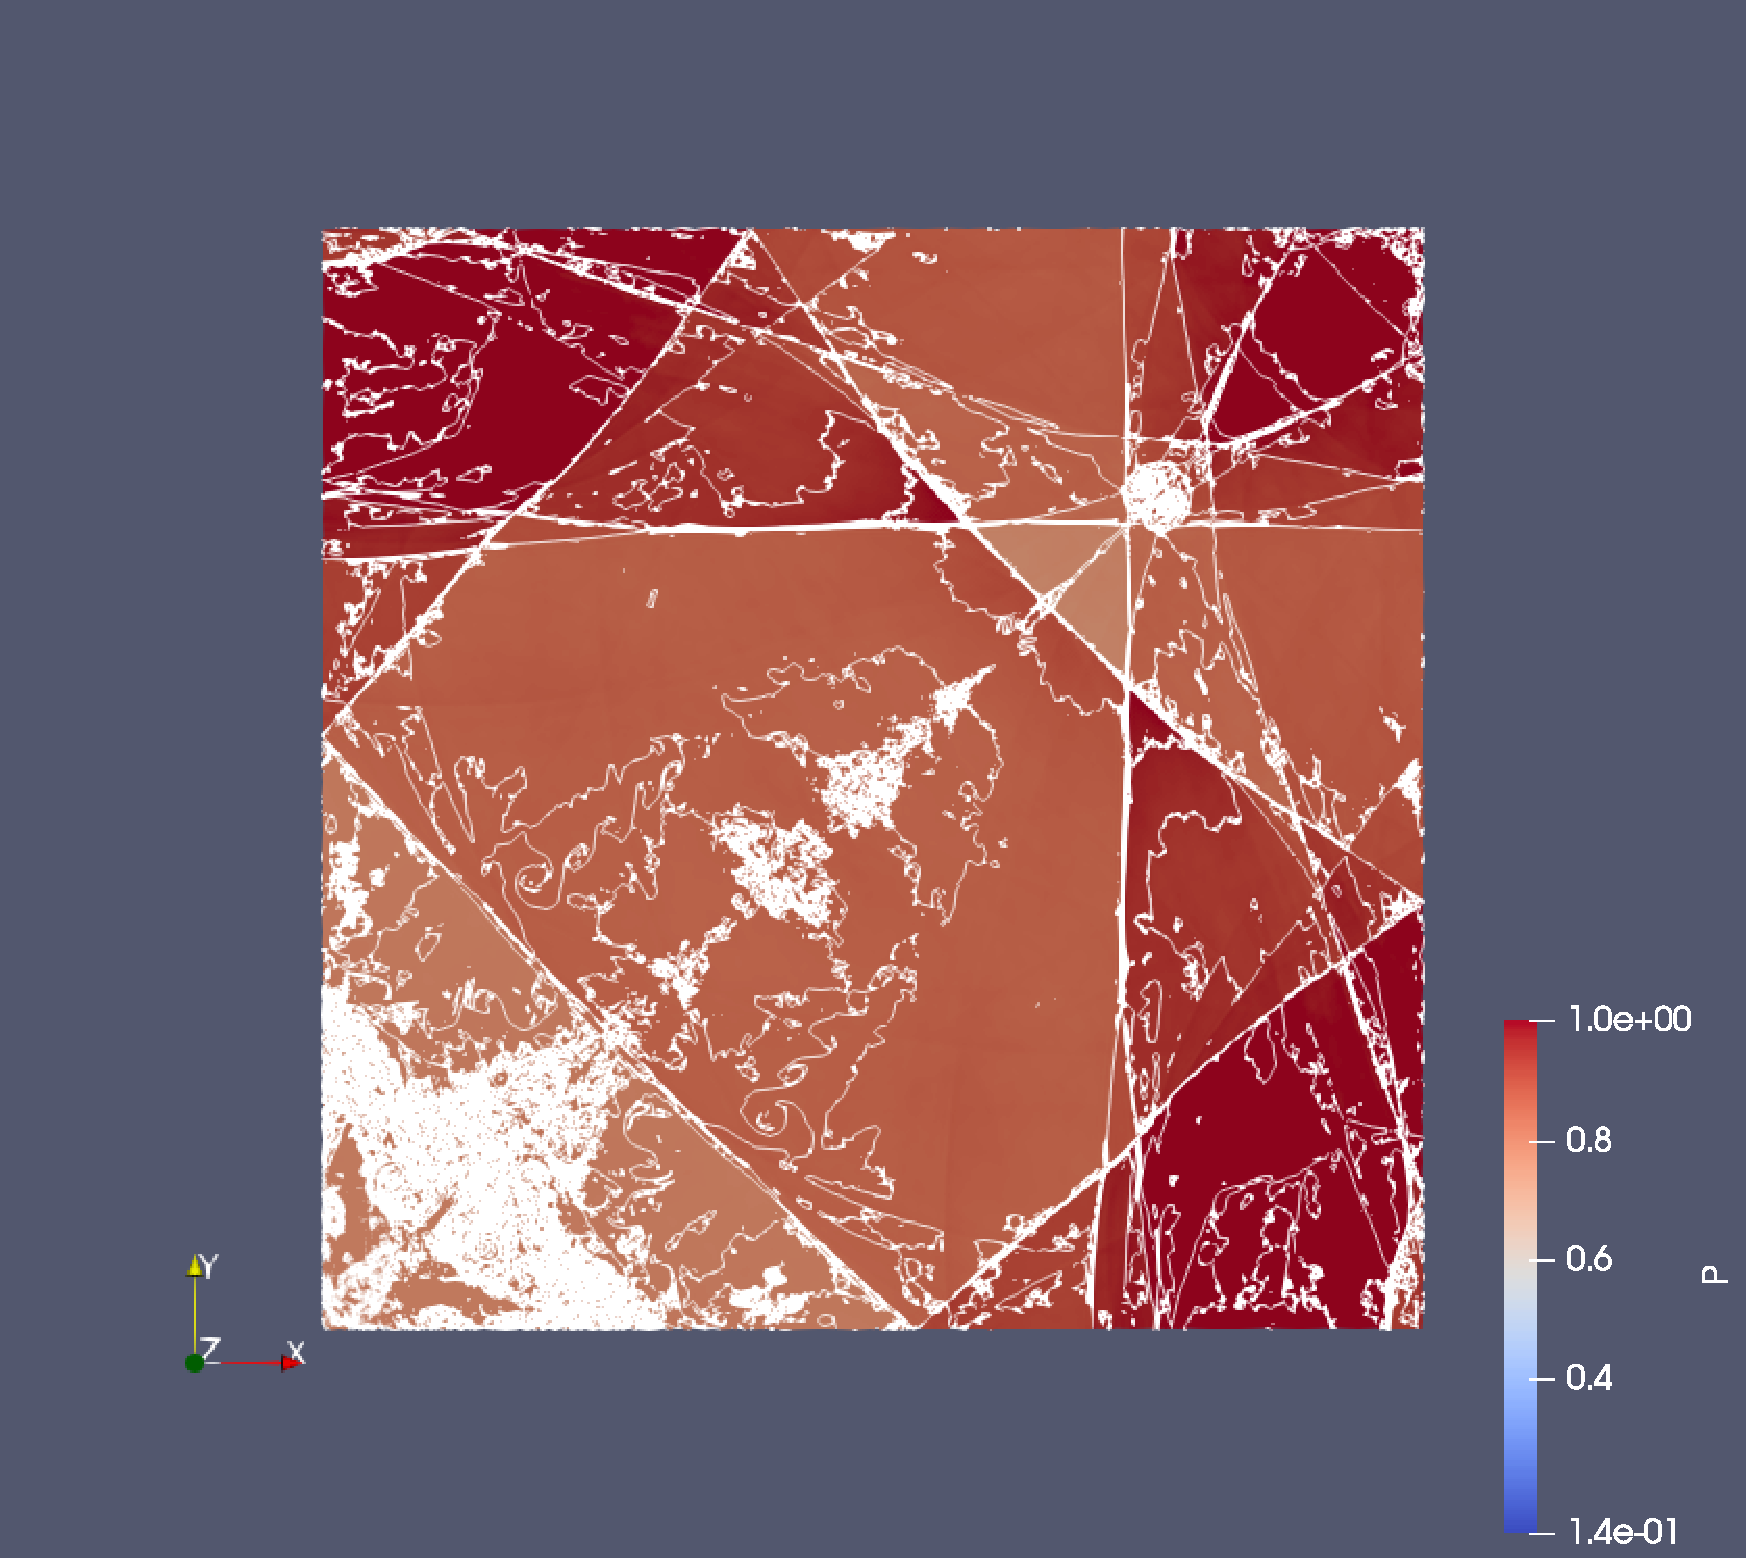
\includegraphics[scale=0.16]{figures/GAH-Hui-400-250.pdf }
\caption{Late time ($t = 2.50$ ) pressure-density results for the $\beta = 0.$ Hui problem. Density contours show values of $\rho$ in $31$ intervals from $0.35$ to $1.1$.}
  \label{fig:hui-Rot0-250}
\end{subfigure}
\caption{The unrotated Hui Problem results.}
\label{fig:hui-Rot0}
\end{figure}

\subsubsection{Rotated mesh}\label{sssec:huiRot}

The results in Figure \ref{fig:hui-Rot} document the case where the box geometry is rotated by $0.4 \ \mathrm{rad}.$ about the $X(3)$ (z coordinate) axis.  The mesh input deck is shown in \ref{ssec:hoprin-hui-Rot} and the Flexi input in \ref{ssec:flexiin-hui-Rot}. The scheme used in the unrotated case (Section \ref{sssec:huiNR})  to assure that the Persson indicator was symmetric about the diagonal line $\overline{42}$ of Figure \ref{fig:HuiGeom} was not used ($\mathrm{IndSym} = 0$).

\begin{figure}[h!]
\centering
\begin{subfigure}[h!]{0.4\linewidth}
\centering
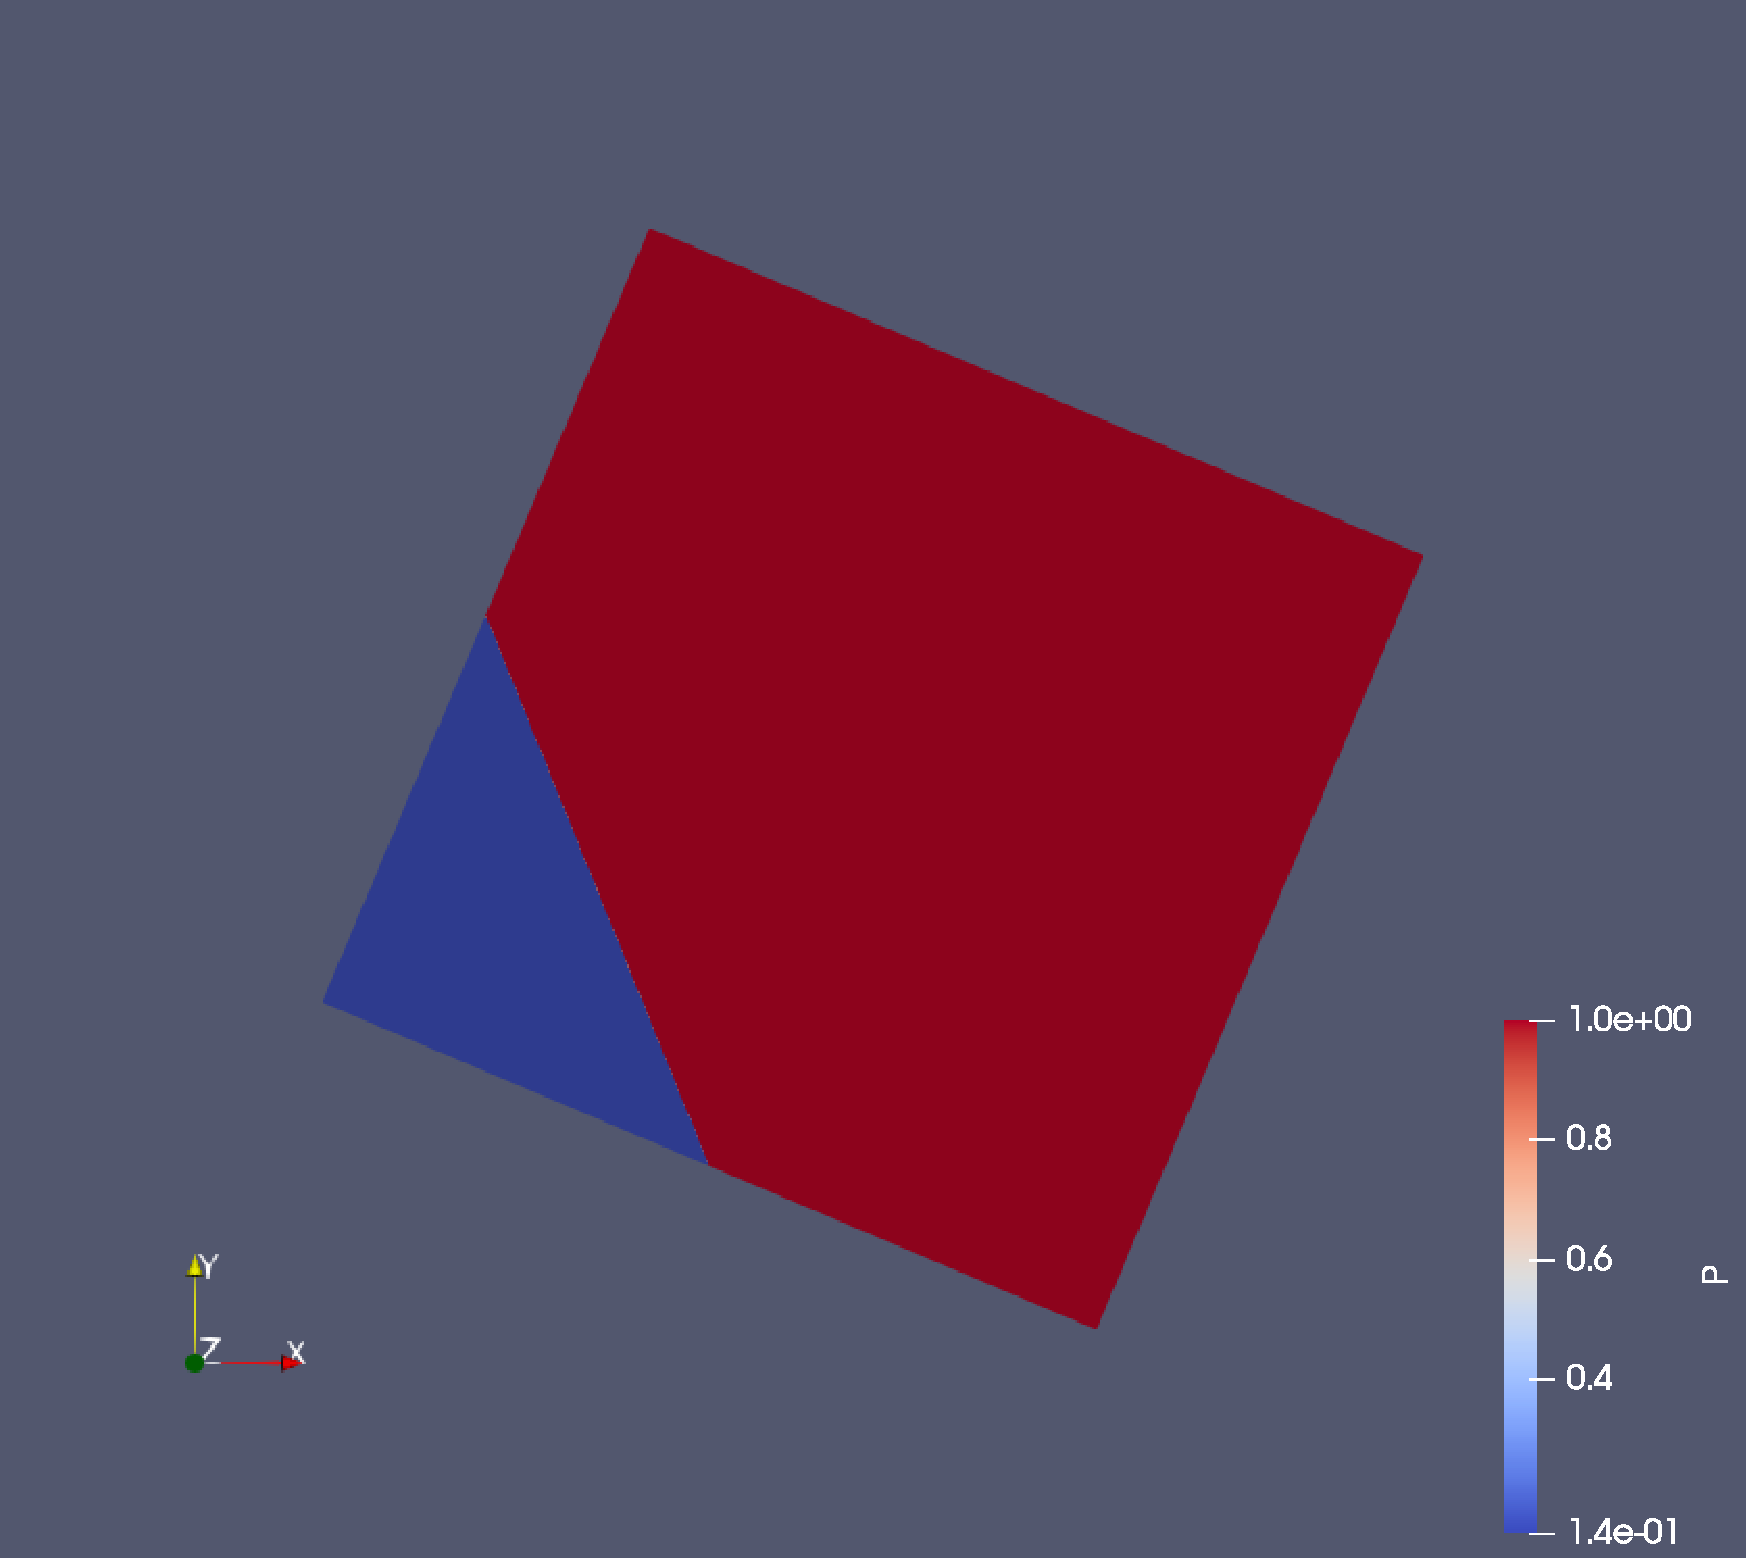
\includegraphics[scale=0.16]{figures/GAH-Hui-400-0000-R.pdf }
\caption{Initial pressure field for the $\beta = 0.4 \ \mathrm{rad.}$ Hui problem.\bigskip \bigskip}
  \label{fig:hui-Rot-0}
\end{subfigure}
\begin{subfigure}[h!]{0.4\linewidth}
\centering
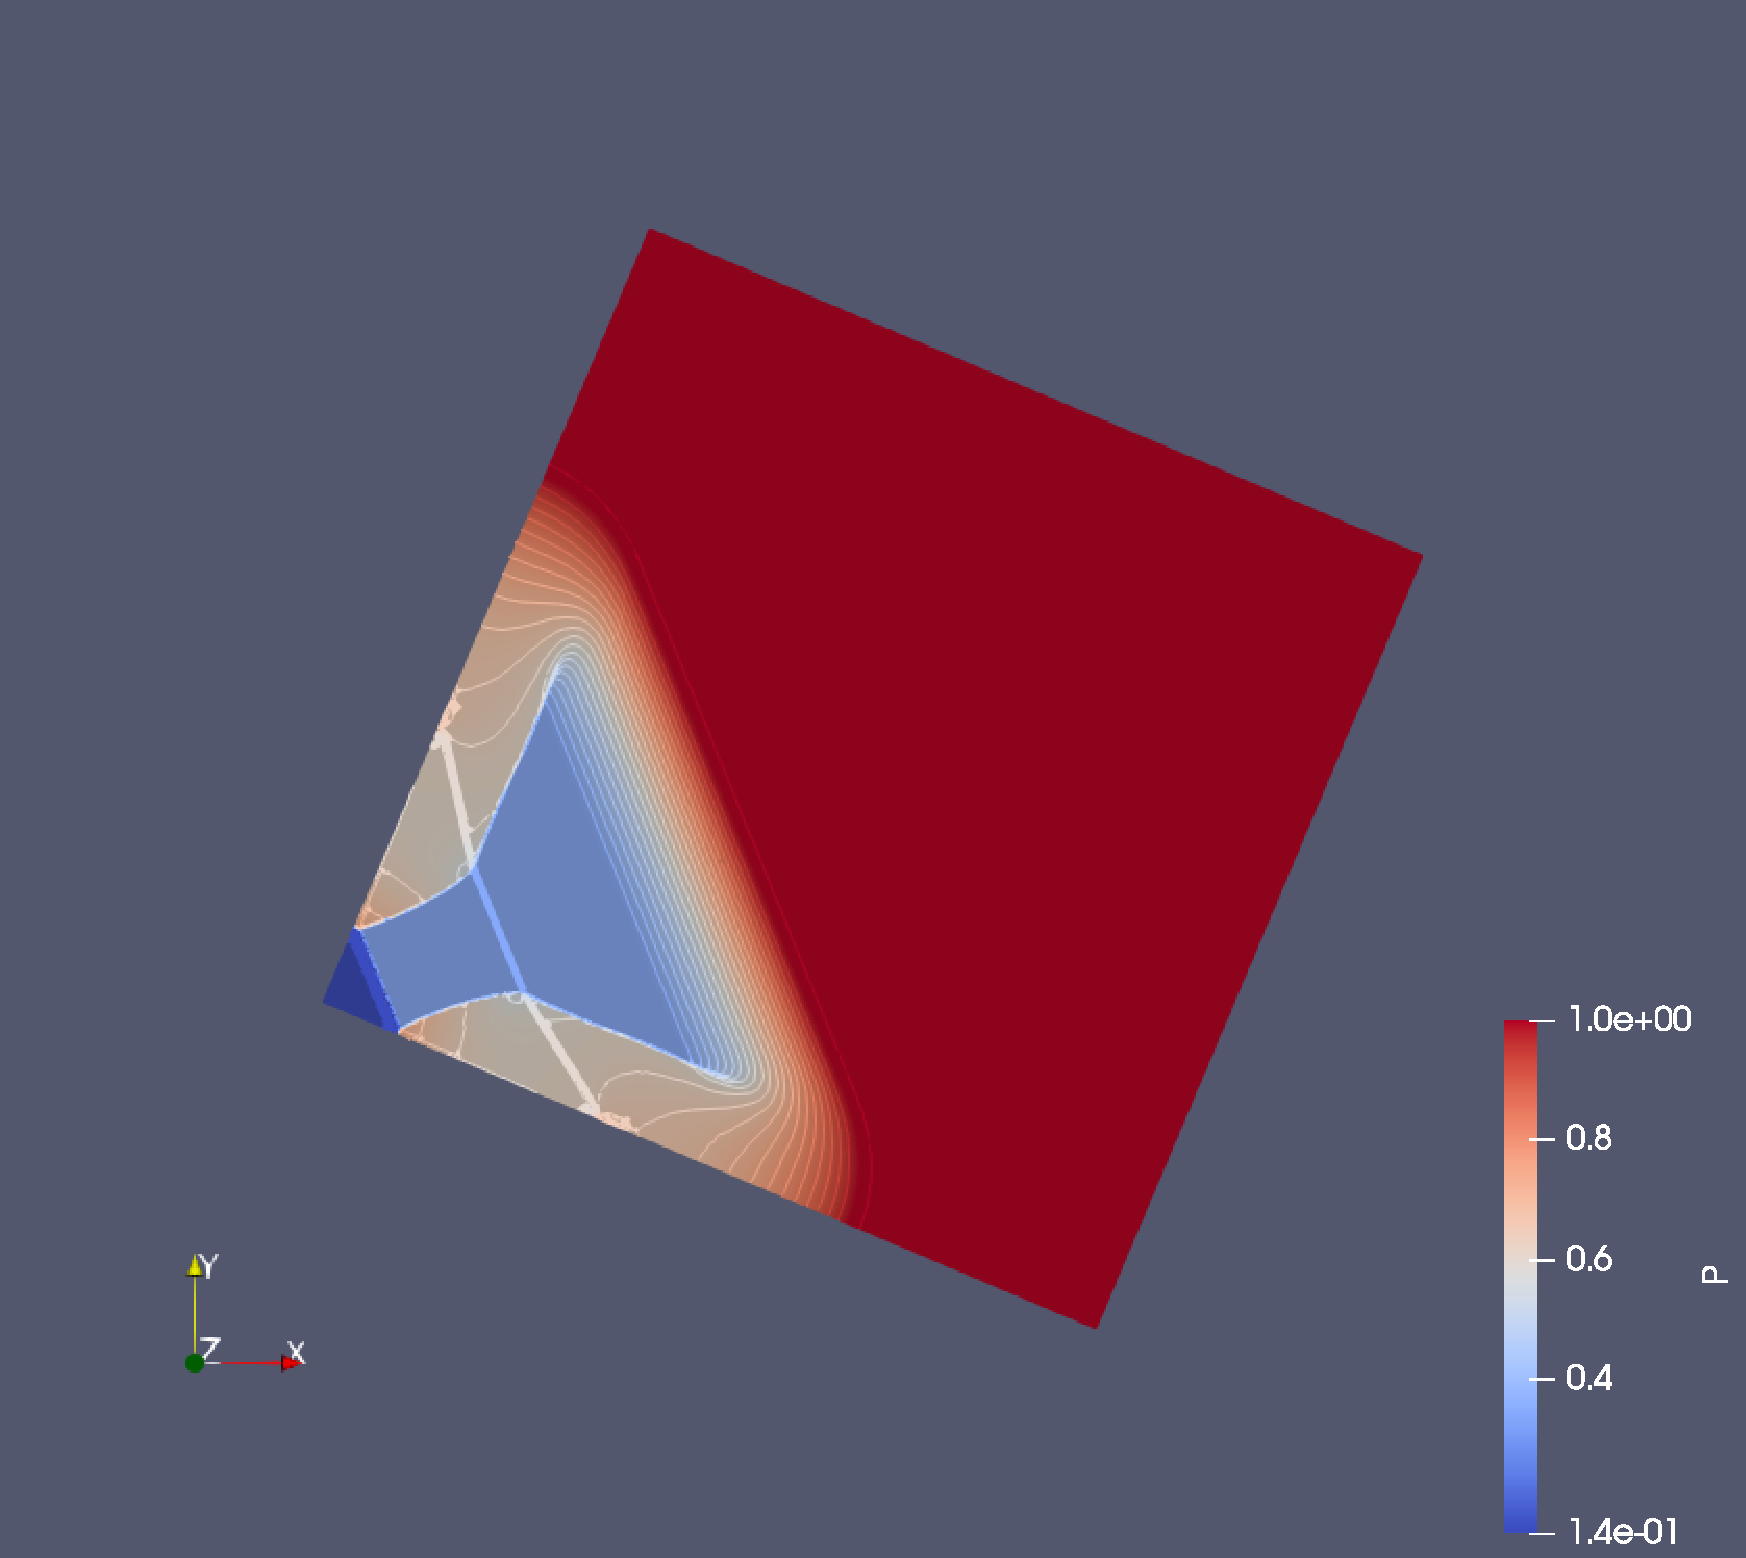
\includegraphics[scale=0.16]{figures/GAH-Hui-400-0045-R.pdf }
\caption{Early time ($t = 0.045$) pressure-density results for the $\beta = 0.4 \ \mathrm{rad.}$ Hui problem. Density contours show values of $\rho$ in $36$ intervals from $0.125$ to $1.0$.}
  \label{fig:hui-Rot-0045}
\end{subfigure}

\bigskip

\begin{subfigure}[h!]{0.4\linewidth}
\centering
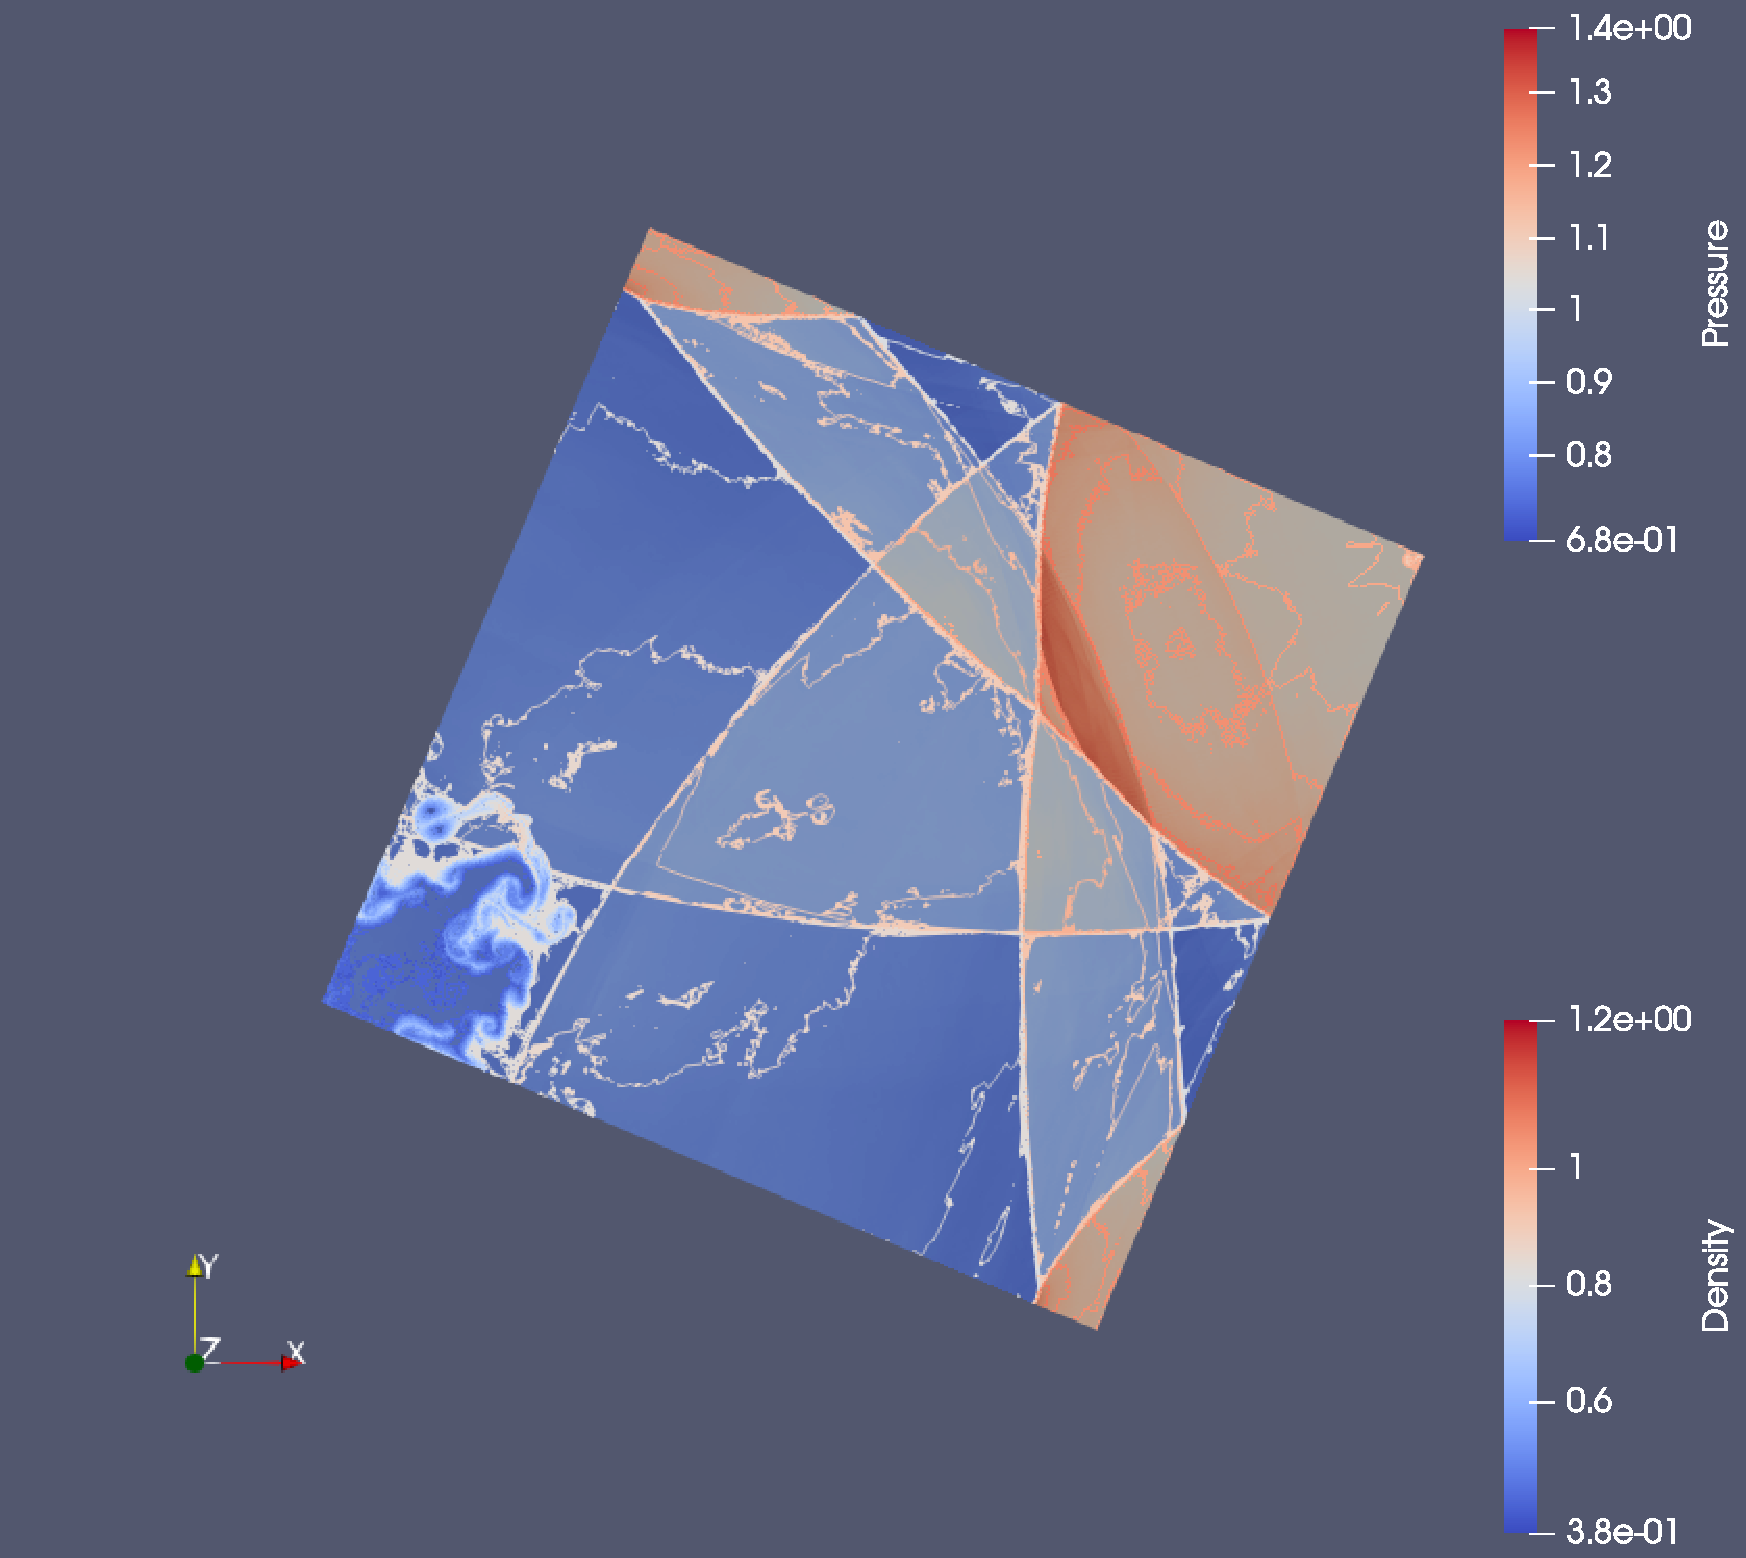
\includegraphics[scale=0.16]{figures/GAH-Hui-400-0100-R.pdf }
\caption{Early time ($t = 0.1$ ) pressure-density results for the $\beta = 0.4 \ \mathrm{rad.}$ Hui problem. Density contours show values of $\rho$ in $31$ intervals from $0.35$ to $1.1$.}
  \label{fig:hui-Rot-250}
\end{subfigure}
\begin{subfigure}[h!]{0.4\linewidth}
\centering
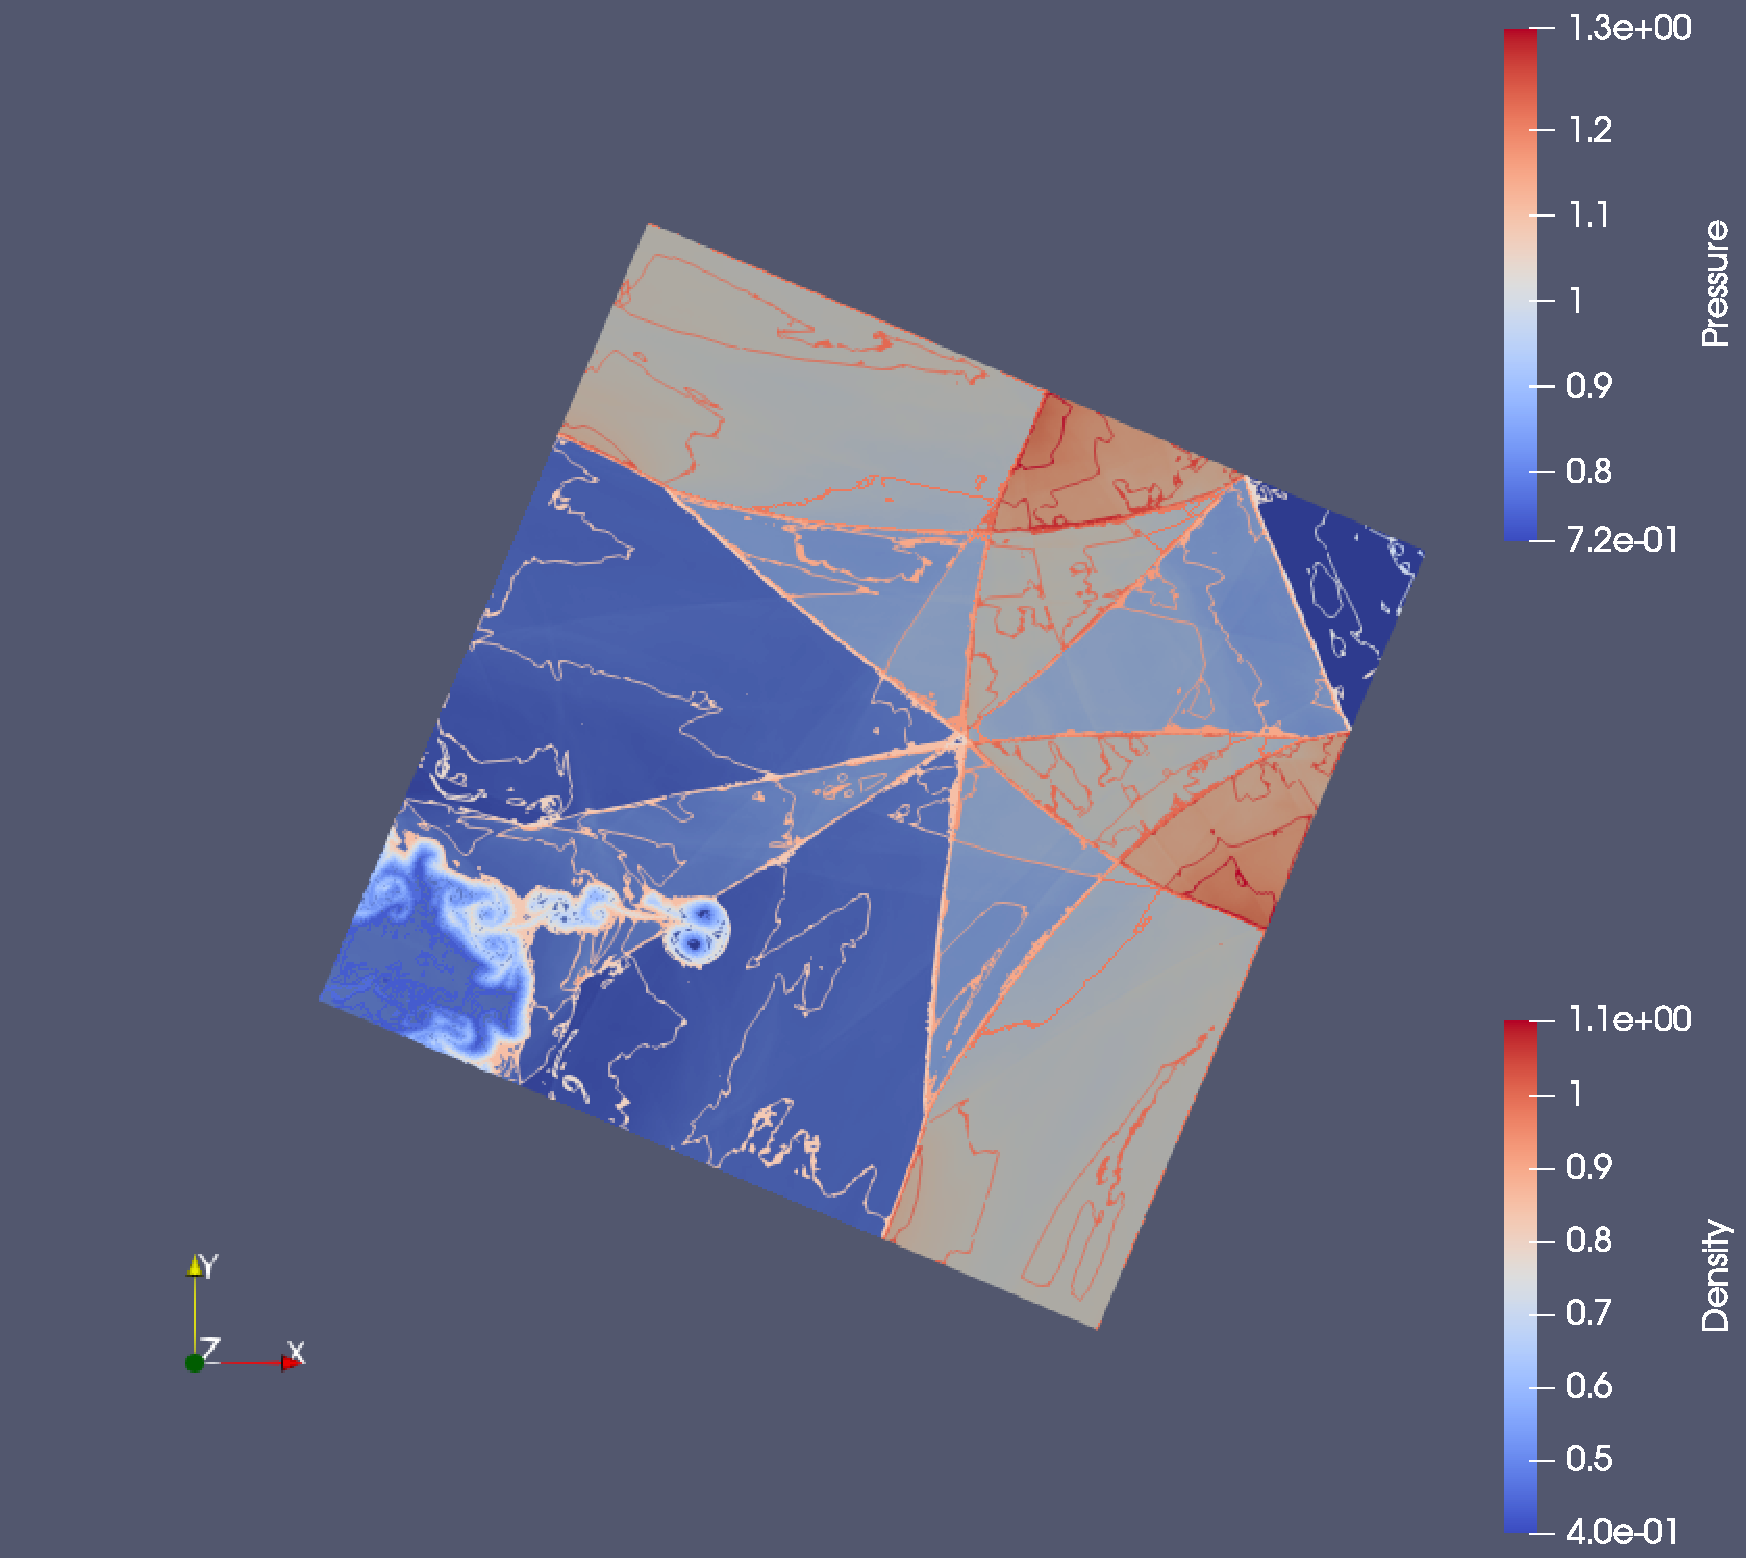
\includegraphics[scale=0.16]{figures/GAH-Hui-400-1500-R.pdf }
\caption{Later time ($t = 1.50$ ) pressure-density results for the $\beta = 0.4 \ \mathrm{rad.}$ Hui problem. Density contours show values of $\rho$ in $31$ intervals from $0.35$ to $1.1$.}
  \label{fig:hui-Rot-1500}
\end{subfigure}

\caption{The rotated Hui Problem results showing asymmetry in the longer time results.  These results did not use the symmetric indicator routine; which gave equally inaccurate results.}
\label{fig:hui-Rot}
\end{figure}

The Hui problem is a very challenging one and Flexi has demonstrated its ability to do well in simulating the problem.  The issues with the rotated mesh results suggests some further review of the code may be necessary.


\section{Conclusions}

As a general statement, Flexi has done an excellent job executing these one- and two-dimensional Riemann problems.  The dual discontinuous Galerkin and finite volume schemes work very well together to focus on discontinuities in the flow field.


\begin{appendices}

\renewcommand\thefigure{\thesection.\arabic{figure}}

\appendix
\section{Compiling Flexi and Hopr}\label{Asec:compile}

\begin{enumerate}
 \item Build Flexi: The following steps assume a Linux operating system running bash.
 \begin{itemize}
 \item Be careful to read the README.md and INSTALL.md files to be sure the dependent libraries are available to the compiler/linker.  In particular, be sure the ``libopenmp-dev'' /library is installed and available for both Flexi and Hopr.
  \item In the directory where you want the source code for Flexi to reside type: git clone \url{https://github.com/flexi-framework/flexi.git} (or else download the ZIP file).
  \item Change directories to the new flexi-directory just created by ''git``. In that top-level Flexi directory, make a new directory called ''build`` and change directory to that directory. Create a new text file (shell script) called, for example, ''do-config`` (using the cases in \ref{sec:configFiles} as examples or by following the Flexi Project Documentation guidance) including the first line: ''\#!/bin/sh`` and the last lines ''$\backslash$" and ``..'' as shown. The flags given there are those needed to compute the compressible flow results given above. Save the file and, since it is a bash-script type: ``chmod u+x do-config'' so it can be executed.  Then, type: ``./do-config'', which runs cmake on the proper files.  (Check the github Flexi site for a complete description of how to build the code as well as any needed dependancies to be sure your computer has all the libraries needed; particularly all the ``mpi'' libraries.)
  \item With successful completion of the prior step, then simply type: ``make'' to build the code.  The executables will reside in the build directory. Note that during the compile step, hdf5-files may be downloaded and compiled (ignore the many compile warnings) if a system wide hdf5-library cannot be found by cmake.
 \end{itemize}
\item Build Hopr: Hopr is a mesh generation code available using: ``git clone \url{https://github.com/flexi-framework/hopr.git}''.  It generates a \.h5 mesh file using a parameter\_hopr.ini file as shown, for example, in \ref{ssec:hoprin-sod1}.
\begin{itemize}
 \item Again, be sure to read the INSTALL.md file at \url{https://github.com/flexi-framework/hopr/blob/master/INSTALL.md} to be sure all dependent libraries are available.  Then, follow the steps given in that document.
\end{itemize}
\end{enumerate}

\section{Flexi Compile Configuration Files}\label{sec:configFiles}

\subsection{Basic Configuration Without posti\_visu}\label{ssec:1Dconfig}
\verbatiminput{inputFiles/do-configure-riemann}

\subsection{Basic Configuration With posti\_visu}\label{ssec:1DconfigPosti}\verbatiminput{inputFiles/do-configure-sod}

\subsection{Two-Dimensional Configuration}\label{ssec:2Dconfig}
\verbatiminput{inputFiles/do-configure-2D}

\section{Running Flexi and Visualizing Solutions: ParaView}\label{sec:paraview}
\setcounter{figure}{0}

The ParaView~[\cite{ParaView},\cite{ParaViewManual}] data analysis and visualization application is used to visualize the solution data from Flexi.  When executing Flexi it is recommended to create a directory to hold the specific files for mesh and input data describing the problem at hand as well as a  ``data'' subdirectory to hold the Flexi output files. Flexi requires an input file usually named ``parameter\_flexi.ini'' and a ``parameter\_hopr.ini``file.  Flexi uses the hopr (High Order Prepriocessor) code (available at \url{https://github.com/flexi-framework/hopr}) code to generate unstructured meshes for a Flexi simulation. Examples of these input files are listed in \ref{Asec:flexiinput} and \ref{Asec:hoprinput}.  Note that the Flexi (and posti\_visu) executables are located in the ''bin`` sub-directory of the build-directory discussed in \ref{Asec:compile}, but hopr has its own directory structure and path to the hopr executable.

With the Flexi ''.ini``  and mesh ''.h5`` files for the current problem, change directory to the ''data`` subdirectory.  This should be an initially empty directory.  (Because the mesh and input files are located up a level be sure the mesh file name in the ''.ini`` file has ''../`` prepended to it.)   Then execute the command:

\begin{verbatim}
path-to-flexi/flexi ../parameter_flexi.ini
\end{verbatim}
\noindent for serial Flexi execution or

\begin{verbatim}
 mpirun -np #processors path-to-flexi/flexi ../parameter_flexi.ini
\end{verbatim}
\noindent Flexi will then run, generating output files with possible extensions of \verb|.h5|, \verb|.vtu|, \verb|.vtm|, and \verb|.pvd| as discussed in Section\ref{sec:files}.

\subsection{Flexi output}\label{sec:files}
The output data files from a Flexi execution depend on the compile flags used, the value of the Flexi input variable ``outputFormat'', and whether or not Flexi (and/or posti\_visu)  is executed serially or in parallel.  The possible output cases are illustrated in Figure~\ref{fig:chart} showing eight possible outcomes. Flexi can generate a number of different output file extensions, depending upon how compilation is done and the input being used, including :

\begin{itemize}
 \item .h5 - HDF5 output for the Flexi current State data generally not readable by ParaView.
 \item .vtu - which usually contain the Discontinuous Galerkin (DG) and in separate Finite Volume (FV) data. These may be readable by Paraview, but displays only the portion of the flow domain using DG or FV.
 \item .vtm - which contains the Solution data which is a combination of the DG and FV data.  These files are readable by ParaView, however if the final execution time is larger the the number $1$ (say, $1.5$) then to get the full animation in ParaView will require a separate code to create the full set of file names for animation.
 \item .pvd - generated when Flexi is run in parallel.
\end{itemize}

\noindent Flexi uses the input variable ``ProjectName'' as a prefix to the output data file names which is in the general form: ``ProjectName\_description\_analizeTime.extension'', for example, Einfeldt-100\_State\_000000.0000000.h5.  File descriptions include: State, FV, DG, and Solution.

Figure~\ref{fig:chart} shows the eight possible Cases for combinations of compilation, execution, and outputFormat which can be used and are described as:

\begin{figure}[h!]
\centering
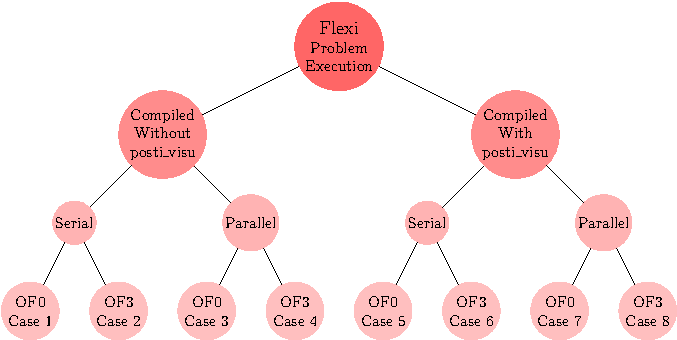
\includegraphics[width=\linewidth]{figures/chart-crop.pdf}
\caption{Output files for Flexi execution depending on the compile flag ``-DPOSTI:BOOL=ON or OFF'', the value of ''outputFile= 0  or 3`` (OF0 or OF3 in the figure), and if execution uses ``mpirun -np \#procs'' (parallel) or not (serial).  There are eight possible combinations represented by Cases 1 through 8.}
\label{fig:chart}
\end{figure}

\begingroup
\renewcommand{\labelenumi}{Case \theenumi:}
\begin{enumerate}
%Case 1
 \item Flexi is compiled with either \verb|-DPOSTI:BOOL=OFF| or omitted from the configure file, Flexi is executed in serial, and ``outputFormat = 0'' or is omitted in the parameter\_flexi.ini file.  In this case, flexi generates ONLY \verb|ProjectName_State_0*.0*.h5| files which are not readable by ParaView.

 %Case 2
 \item Flexi is compiled with either \verb|-DPOSTI:BOOL=OFF| or omitted from the configure file, Flexi is executed in serial, and ``outputFormat = 3'' in the parameter\_flexi.ini file which is the ParaView output option. This case generates the following files:
 \begin{itemize}
  \item \verb|ProjectName_State_0*.0*.h5|
  \item \verb|ProjectName_FV_0*.0*.vtu|
  \item \verb|ProjectName_DG_0*.0*.vtu|
  \item \verb|ProjectName_Solution_0*.0*.vtm|
 \end{itemize}
 \noindent The \verb|.vtm| files are readable by ParaView and has all conserved variables as well as ``FV\_Elems'' and ``IndValue'' available for display in the animation.  These last variables show how Flexi switches between Finite Volume and Discontinuous Galerkin solution methods. They are NOT available for display in ParaView if ``posti\_visu'' is used.

 %Case 3
 \item Flexi is compiled with either \verb|-DPOSTI:BOOL=OFF| or omitted from the configure file, Flexi is executed in parallel using ``mpirun -np \#processors'', and ``outputFormat = 0'' or is omitted in the parameter\_flexi.ini file. This case generates the following files:
 \begin{itemize}
  \item \verb|ProjectName_State_0*.0*.h5|
 \end{itemize}
\noindent which are NOT readable by ParaView.

%Case 4
\item Flexi is compiled with either \verb|-DPOSTI:BOOL=OFF| or omitted from the configure file, Flexi is executed in parallel using ``mpirun -np \#processors'', and ``outputFormat = 3'' in the parameter\_flexi.ini file which is the ParaView output option. This case generates the following files:
 \begin{itemize}
  \item \verb|ProjectName_State_0*.0*.h5|
  \item \verb|ProjectName_FV_0*.0*.vtu|
  \item \verb|ProjectName_DG_0*.0*.vtu|
  \item \verb|ProjectName_Solution_0*.0*.pvd|
 \end{itemize}
\noindent  The solution .pvd files are not readable by ParaView.

% Case 5
\item Flexi is compiled with \verb|-DPOSTI:BOOL=ON| in the configure file, Flexi is executed in serial and ``outputFormat = 0'' in the parameter\_flexi.ini file which is the ParaView output option. This case generates the following files:
 \begin{itemize}
  \item \verb|ProjectName_State_0*.0*.h5|
 \end{itemize}
\noindent  The solution .h5 files are not readable by ParaView. However, these h5-files are converted to ParaView readable files using posti\_visu as discussed in Section~\ref{sec:posti}.

%Case 6
\item Flexi is compiled with \verb|-DPOSTI:BOOL=ON| in the configure file, Flexi is executed in serial and ``outputFormat = 3'' in the parameter\_flexi.ini file which is the ParaView output option. This case generates the following files:
 \begin{itemize}
  \item \verb|ProjectName_FV_0*.0*.vtu|
  \item \verb|ProjectName_DG_0*.0*.vtu|
  \item \verb|ProjectName_Solution_0*.0*.vtm|
  \item \verb|ProjectName_State_0*.0*.h5|
 \end{itemize}
\noindent  The resulting solution .vtm files are readable by ParaView and displays the conserved variables as well as FV\_Elems and \verb|IndValue|.  posti\_visu is not needed in order to display these results.

% Case 7
\item Flexi is compiled with \verb|-DPOSTI:BOOL=ON| in the configure file, Flexi is executed in parallel  using ``mpirun -np \#processors'', and ``outputFormat = 0'' in the parameter\_flexi.ini file. This case generates the following files:
 \begin{itemize}
  \item \verb|ProjectName_State_0*.0*.h5|
 \end{itemize}
\noindent  The solution .h5 files are not readable by ParaView. However, these h5-files are converted to ParaView readable files using posti\_visu as discussed in Section~\ref{sec:posti}.

%Case 8
\item Flexi is compiled with \verb|-DPOSTI:BOOL=ON| in the configure file, Flexi is executed in parallel  using ``mpirun -np \#processors'', and ``outputFormat = 3'' in the parameter\_flexi.ini file which is the ParaView output option. This case generates the following files:
 \begin{itemize}
  \item \verb|ProjectName_FV_0*.0*.vtu|
  \item \verb|ProjectName_DG_0*.0*.vtu|
  \item \verb|ProjectName_Solution_0*.0*.pvd|
  \item \verb|ProjectName_State_0*.0*.h5|
 \end{itemize}
\noindent  The resulting solution .pvd files are not readable by ParaView.  However, posti\_visu will generate readable ParaView data as discussed in Section~\ref{sec:posti}.

\end{enumerate}
\endgroup
\noindent These data are summarized in Table~\ref{tab:cases}.

\begin{table}[h!]
 \centering
 \tiny
 \caption{Summary of output files generated when Flexi is executed in either serial or parallel and depending on whether or not Flexi is compiled with posti\_visu and if the outputFormat is set to either 0 or 3 in the Flexi input file. ParaView readability is noted: if ``Yes'', then all conserved variables, FV\_Elems and IndValue are available for display, if ``Yes (w/o FV\_Elems)'' means that only conserved variables are available, if ``Only discrete time pvd's'' then pvd files are readable, but only one time step at a time, while if ``NO'', ParaView gives errors when input files are read. vtm files are always readable and for all time steps so that animation is displayable in ParaView. Using posti\_visu in serial always produces vtm files, but without FV\_Elems and IndValue data.}\label{tab:cases}
 \begin{tabular}{|c|c|c|c|c|c|} \hline
  \multirow{3}{*}{Case} & -DPOSTI & Flexi: Serial(S)/Parallel(P) & Output & Solution & ParaView \\ \cline{3-3}
   & Compile & posti\_visu: Serial (S) & Format & Extensions & Readable \\
   & Flag & posti\_visu: Parallel (P)&  & & \\ \hline
% Case 1
 \multirow{3}{*}{1} & \multirow{3}{*}{OFF} & S & \multirow{3}{*}{0} & h5 & No \\ \cline{3-3} \cline{5-6}
    &  &  N/A & & N/A & N/A \\
    &  &  N/A & & N/A & N/A \\ \hline

% Case 2
 \multirow{3}{*}{2} & \multirow{3}{*}{OFF} & S & \multirow{3}{*}{3} & h5, vtu, vtm & Yes \\ \cline{3-3} \cline{5-6}
     &  &  N/A & & N/A & N/A \\
    &  &  N/A & & N/A & N/A \\ \hline

% Case 3
 \multirow{3}{*}{3} & \multirow{3}{*}{OFF} & P & \multirow{3}{*}{0} & h5 & No \\ \cline{3-3} \cline{5-6}
    &  &  N/A & & N/A & N/A \\
    &  &  N/A & & N/A & N/A \\ \hline

% Case 4
 \multirow{3}{*}{4} & \multirow{3}{*}{OFF} & P & \multirow{3}{*}{3} & h5, vtu, pvd & No \\ \cline{3-3} \cline{5-6}
   &  &  N/A & & N/A & N/A \\
    &  &  N/A & & N/A & N/A \\ \hline

% Case 5
\multirow{3}{*}{5} & \multirow{3}{*}{ON} & S & \multirow{3}{*}{0} & h5 & No \\ \cline{3-3} \cline{5-6}
    &  &  S & & vtu, vtm & Yes (w/o FV\_Elems) \\
    &  &  P & & pvtu, pvd, vtu & Only discrete time pvd's \\ \hline

% Case 6
\multirow{3}{*}{6} & \multirow{3}{*}{ON} & S & \multirow{3}{*}{3} & h5, vtu, vtm & Yes \\ \cline{3-3} \cline{5-6}
   &  &  S & & vtu, vtm & Yes (w/o FV\_Elems) \\
    &  &  P & & pvtu, pvd, vtu & Only discrete time pvd's \\ \hline

% Case 7
\multirow{3}{*}{7} & \multirow{3}{*}{ON} & P & \multirow{3}{*}{0} & h5 & No \\ \cline{3-3} \cline{5-6}
   &  &  S & & vtu, vtm &  Yes (w/o FV\_Elems) \\
    &  &  P & & pvtu, pvd, vtu & Only discrete time pvd's  \\ \hline

% Case 8
\multirow{3}{*}{8} & \multirow{3}{*}{ON} & P & \multirow{3}{*}{3} & h5, vtu, pvd & No \\ \cline{3-3} \cline{5-6}
   &  &  S & & vtu, vtm & Yes  (w/o FV\_Elems)  \\
  &   &  P & & pvtu, pvd, vtu & Only discrete time pvd's \\ \hline
 \end{tabular}
\end{table}

\subsection{posti\_visu Post Processing}\label{sec:posti}

When Flexi is finished, Paraview~[\cite{ParaView}] can be used to visualize the transient results and will require a group of \verb|.vtm| or \verb|.pvd| input files.  Flexi provides a tool called posti\_visu which converts Flexi State files to ParaView input files, which (assuming execution is in the data subdirectory mentioned above) can be generated using the command:

\begin{verbatim}
 path-to-posti_visu/posti_visu ../parameter_flexi.ini \
    ./ProjectName_State.000000*.*.h5
\end{verbatim}
\noindent for serial execution of posti\_visu or

\begin{verbatim}
 mpirun -np #processors path-to-posti_visu/posti_visu \
     ../parameter_flexi.ini ./ProjectName_State.000000*.*.h5
\end{verbatim}
\noindent for parallel execution of posti\_visu, where ''ProjectName``  is defined in the \verb|parameter_flexi.ini| file using the \verb|ProjectName =| variable.  This way of executing posti\_visu gives the default output: the conserved variables listed in Table~\ref{tab:flexiVars}.  If primitive varables are desired to be displayed either use the ParaView Calculator application discussed in Section~\ref{sec:usingParaView} or a parameter\_postiVisu.ini file can be created using the primitive variable names given in Table~\ref{tab:flexiVars} according to the directions in Section 5.10 of the Flexi Project Documentation (\textit{c.f.,} Flexi Project Documentation in the ''references`` directory) and shown in the following example:

\begin{verbatim}
nvisu = 10
varname=Density
varname=Pressure
varname=VelocityX
varname=EnergyStagnation
varname=Mach
varname=EnthalpyStagnation
\end{verbatim}

\subsection{Using ParaView}\label{sec:usingParaView}

ParaView should be already installed on your computer and available in the \verb|$PATH|-environment variable. Open paraview in the ``data'' subdirectory and load the solution \verb|.vtm| file group as shown in Figure\ref{fig:openPV} and \ref{fig:applyPV}. Because of ParaView's interpretation of the input time stamp for each .vtm file, say a tool is available (\textit{c.f.,} the \textbf{tools/makePVD/ directory}) called makepvd.py which will create a new input file with all output residing in one file.  This is particularly relevent when the final stop time for Flexi is $\ge 1.$ The dependent variables of the solution are listed in the Properties window and may be selected for transient display using the ``Solid Color'' drop-down menu above the display.  For example, selecting density and clicking on the green right-arrow button, the density is shown at each solution time step (\textit{e.g.,} Figure \ref{fig:DensityField})

% Read ParaView files
\begin{figure}
\centering
\begin{subfigure}{.95\textwidth}
  \centering
  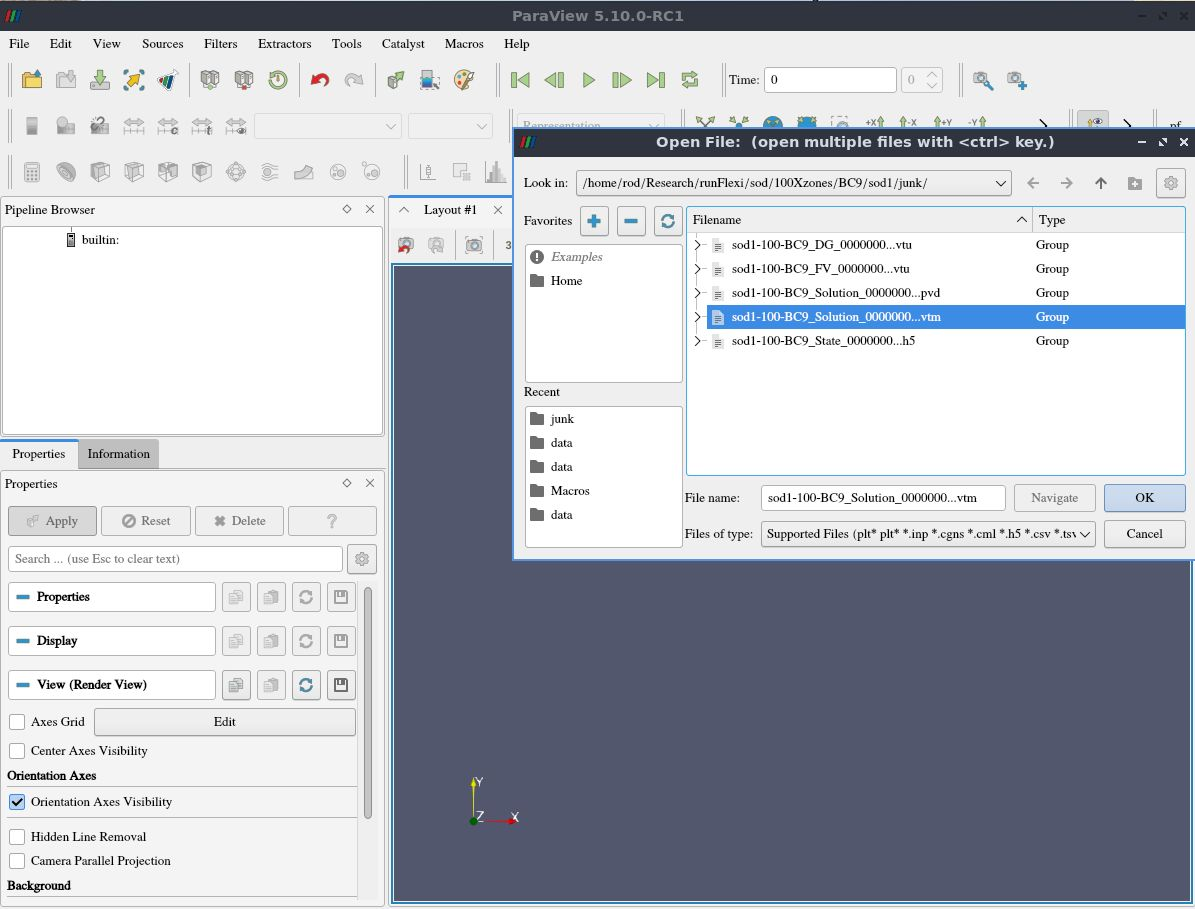
\includegraphics[width=.9\linewidth,height=0.9\linewidth,scale=1]{figures/paraviewGrabs/OpenFiles.jpg}
  \caption{Open the .vtm file group in ParaView}
  \label{fig:openPV}
\end{subfigure}
\begin{subfigure}{.95\textwidth}
  \centering
  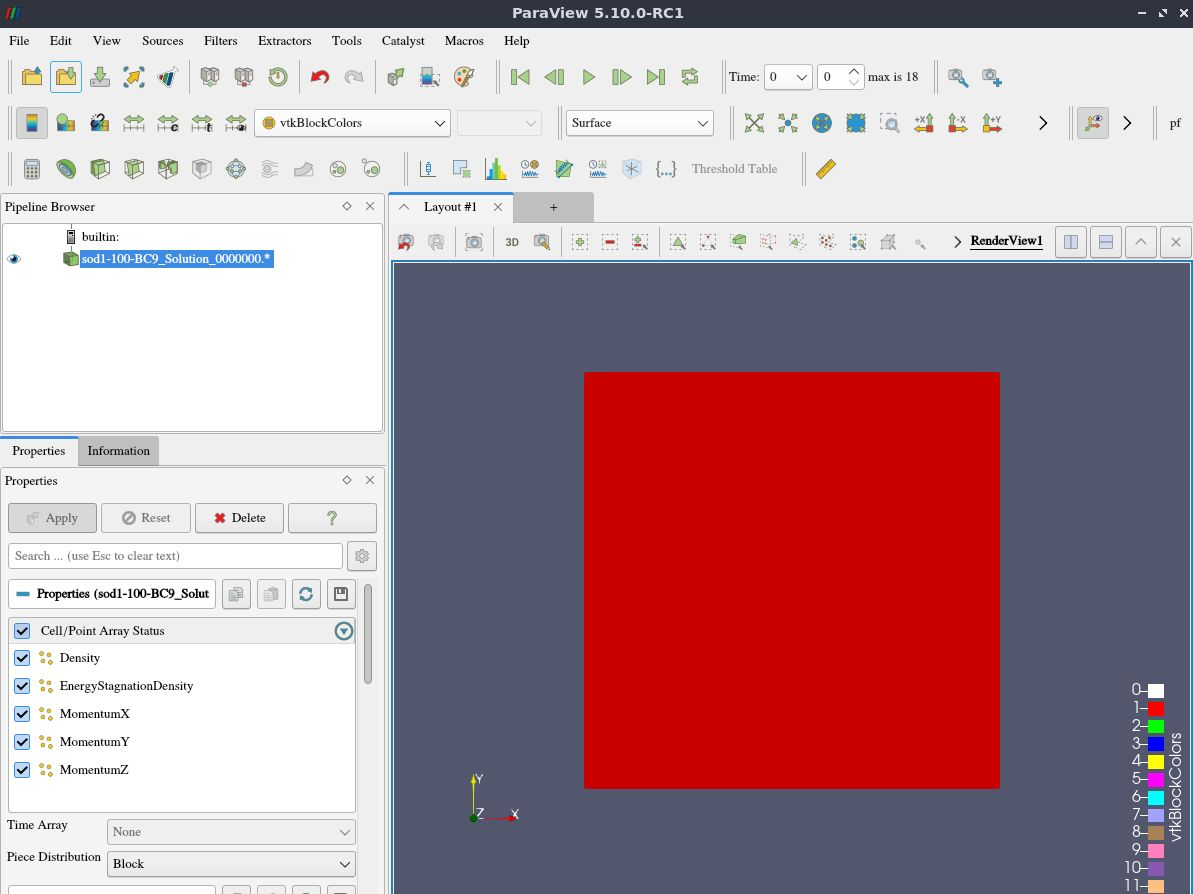
\includegraphics[width=.9\linewidth,height=0.9\linewidth,scale=1]{figures/paraviewGrabs/AfterApply-openfile.jpg}
  \caption{ParaView display after opening data files and clicking Apply in the Properties window.}
  \label{fig:applyPV}
\end{subfigure}
\end{figure}

\begin{figure}[ht]\ContinuedFloat
\centering
\begin{subfigure}{.95\textwidth}
  \centering
  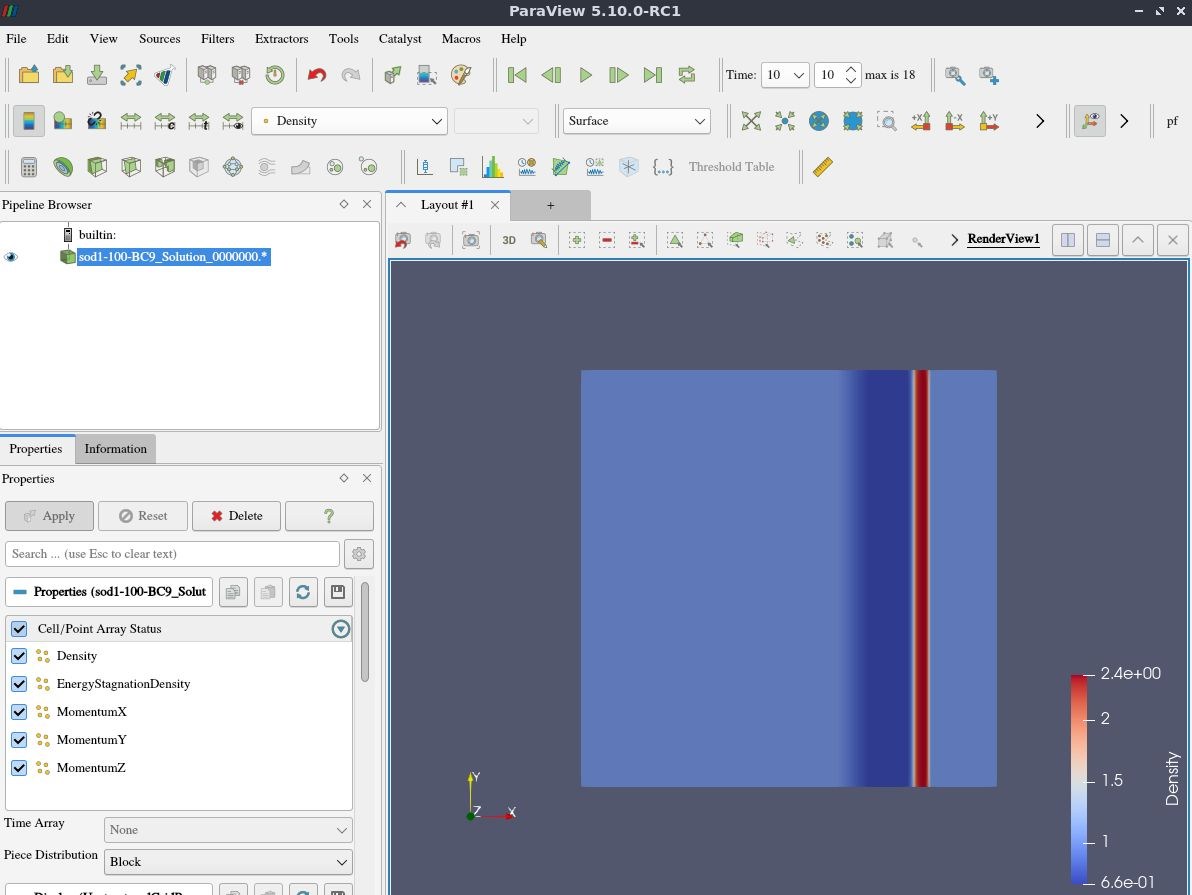
\includegraphics[width=.9\linewidth,height=0.9\linewidth,scale=1]{figures/paraviewGrabs/DensityField.jpg}
  \caption{The Density field displayed at the $10^{th}$ time step in the solution.}
  \label{fig:DensityField}
\end{subfigure}
\caption{ParaView: Reading Flexi simulation data files.}
\label{fig:PVopenFile}
\end{figure}

% Use Calculator app to create new variables

Because Flexi uses Density, MomentumX, MomentumY, MomentumZ, and EnergyStagnationDensity as the conserved solution variables primitive variables like pressure, internal energy, and x-velocity can be computed in ParaView using the Calculator application found in the Filters $\rightarrow$ Common menu located at the top line of the display.  For example, Figure \ref{fig:CalcXvel} shows that once the Calculator app is started, a new entry appears in the Pipeline Browser under the solution data and a new window opens in the Properties tab.  Either Cell or Point Data can be selected (depending on the type of data read in) and next to the ``Result Array Name'' is a box in which a new variable name is entered.  In the Figure, ``xvel'' is entered and in the next box below is entered the equation to convert ``MomentumX'' to ``xvel'' by dividing by ``Density''.  Each variable name can be either typed in or selected from the Scalars or Vectors menu at the bottom.  Clicking on Apply does the calculation and makes the new variable ``xvel'' available for plotting or use in other Calculators. Additional primitive variables are shown in Figures\ref{fig:CalcEint}, \ref{fig:CalcPres} and \ref{fig:CalcC} for specific internal energy, pressure, and sound speed, respectively.

\begin{figure}
\centering
\begin{subfigure}{.95\textwidth}
  \centering
  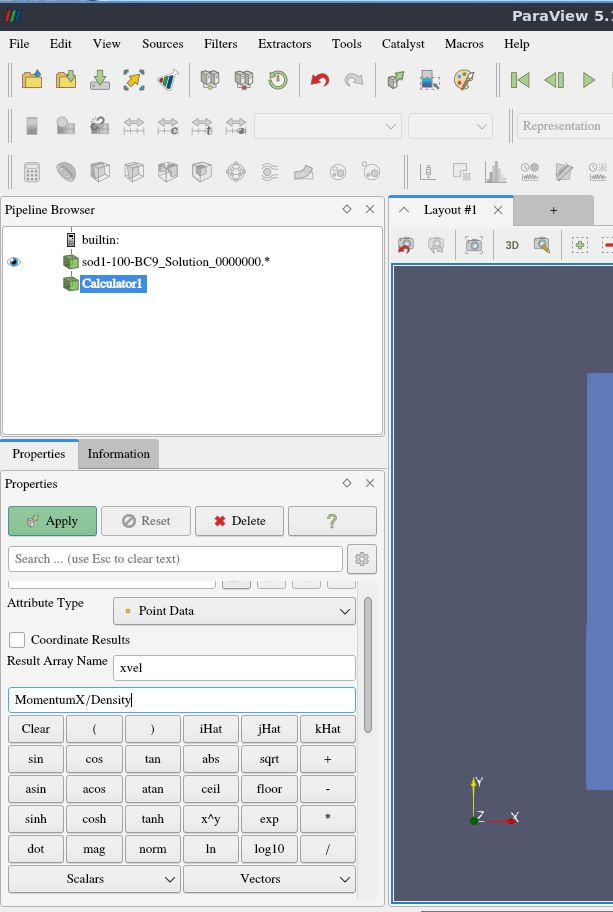
\includegraphics[width=.9\linewidth,height=0.9\linewidth,scale=1]{figures/paraviewGrabs/CalculatorXvel.jpg}
  \caption{Use the Calculator app to calculate the x-velocity.}
  \label{fig:CalcXvel}
\end{subfigure}
\begin{subfigure}{.95\textwidth}
  \centering
  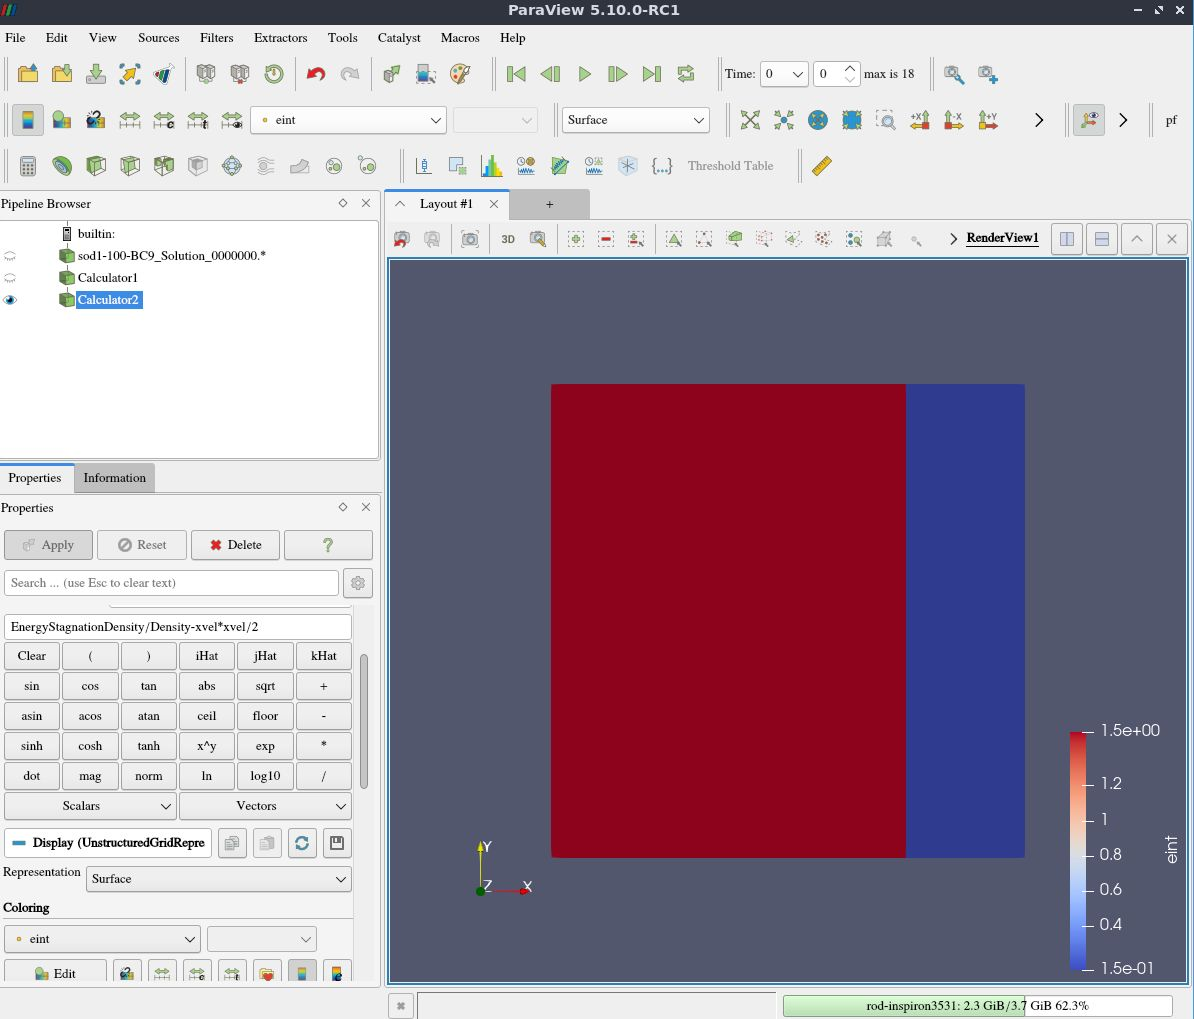
\includegraphics[width=.9\linewidth,height=0.9\linewidth,scale=1]{figures/paraviewGrabs/CalculatorEint.jpg}
  \caption{Use the Calculator app to calculate the specific internal energy.}
  \label{fig:CalcEint}
\end{subfigure}
\end{figure}

\begin{figure}\ContinuedFloat
\centering
\begin{subfigure}{.95\textwidth}
  \centering
  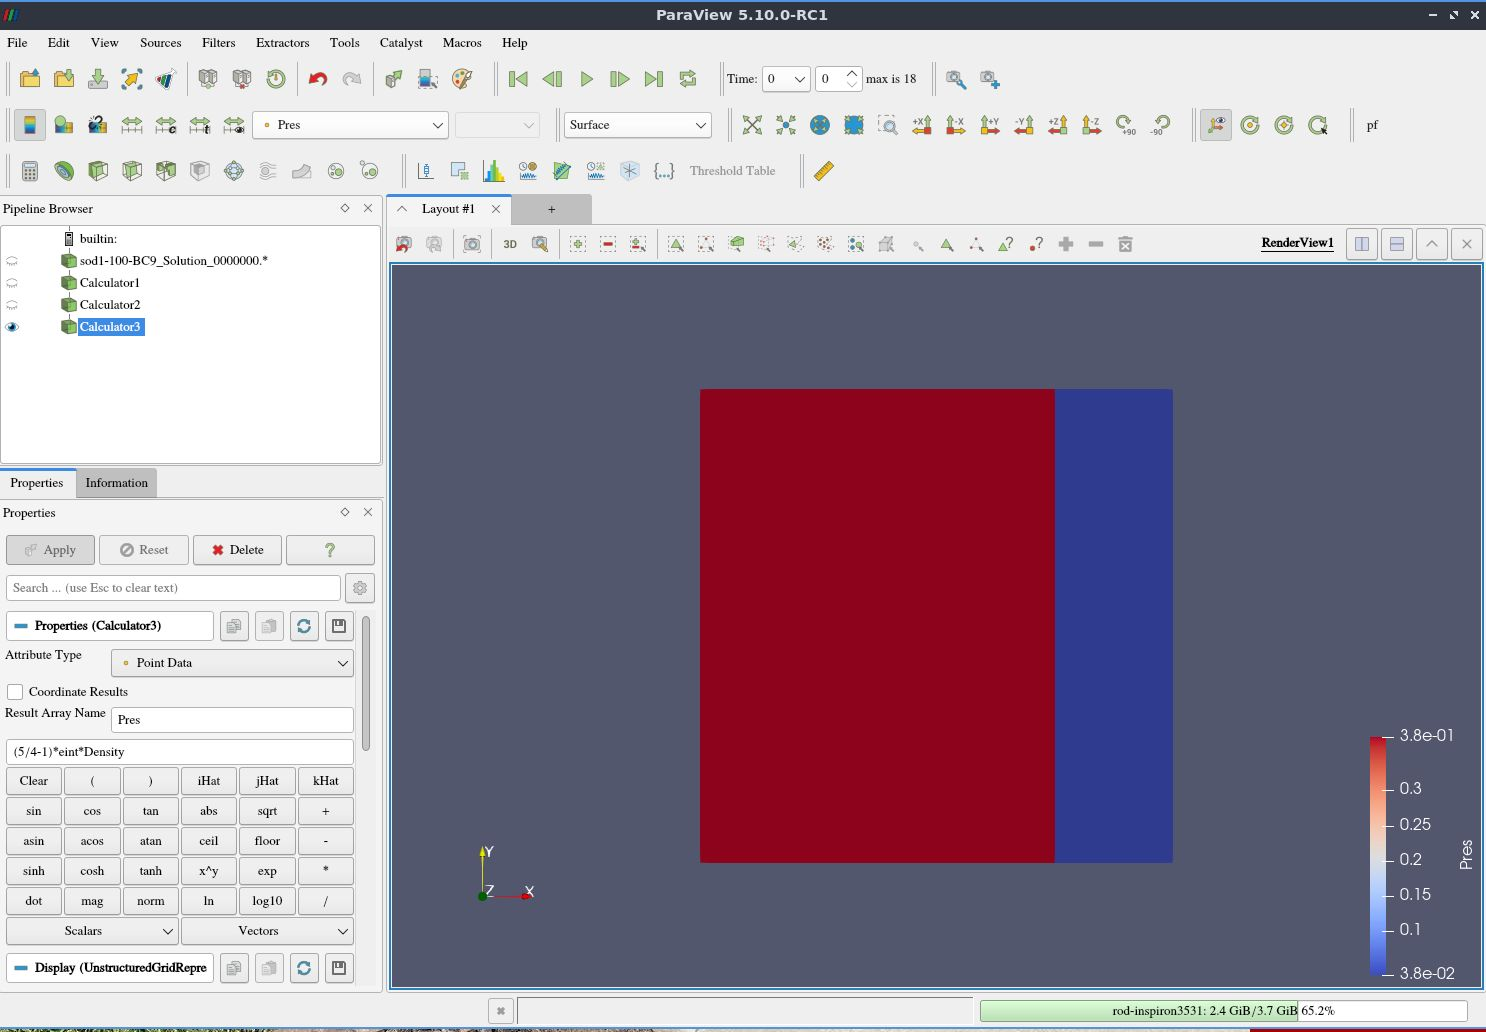
\includegraphics[width=.9\linewidth,height=0.9\linewidth,scale=1]{figures/paraviewGrabs/CalculatorPres.jpg}
  \caption{Use the Calculator app to calculate the pressure.}
  \label{fig:CalcPres}
\end{subfigure}
\begin{subfigure}{.95\textwidth}
  \centering
  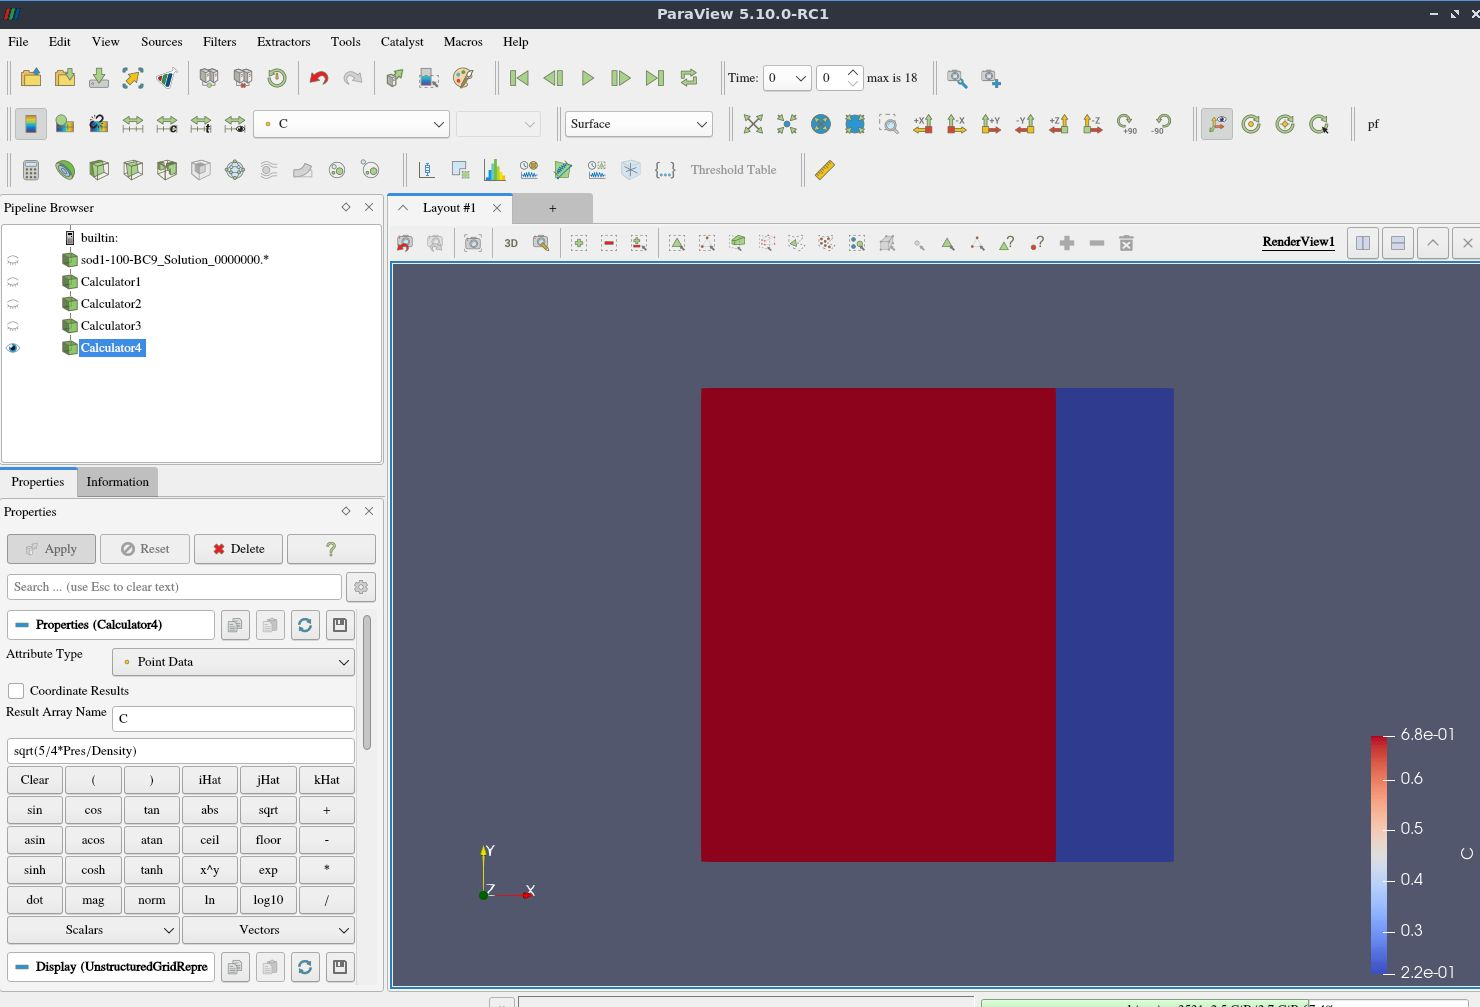
\includegraphics[width=.9\linewidth,height=0.9\linewidth,scale=1]{figures/paraviewGrabs/CalculatorC.jpg}
  \caption{Use the Calculator app to calculate the speed of sound.}
  \label{fig:CalcC}
\end{subfigure}
\caption{ParaView: Using the Calculator app to compute primative variables.}
\label{fig:CalcExamples}
\end{figure}

For one dimensional problems as computed in a three dimension mesh it is often desired to extract line plots of the dependent and/or primitive variables from ParaView displays.  In addition, the plot data may need to be exported so that the numerical data may be used for other analytical purposes.  Using the example in the prior two Figures, the following Figure\ref{fig:POL} shows a way to do these operations. Figure \ref{fig:POL1} shows the display when, from the top row of File, Edit, \textit{etc.} options, the Filters $\rightarrow$ Common $\rightarrow$ plot-over-line app is selected.  In the  ``Properties'' window along the left side under Line Parameters, adjust the Point 1 and Point 2 coordinates to be the end points of the line along which the plot is to be made.  Then click ``Apply'' resulting in the display as shown in Figure \ref{fig:POL2}. A new window called ``LineChartView 1`` opens displaying the plot of all varables available.  (The other window, ''Layout \# 1``, can be closed by clicking on the ''X`` button on the top right corner.) In the ''Properties'' window move the vertical slider nearest the Layout window dow until you see a table of potential display variables.  Select those desired for this line plot (its line color can be changed by double-clicking on the colored button next to the variable name; a new color selection window pops up from which the new color may be chosen.  When done, click on ``Apply'', resulting in a line plot as shown in Figure \ref{fig:POL3}.  To save the actual coordinate and variable data for this line plot, click on the ``File'' pull-down menu at the very top row of the display and select ``Export Scene'', resulting in a new window appearing on the display, as shown in Figure \ref{fig:POL4}.  Here, the directory for the saved data as well as its name and output type are set.  The export can be in comma-separated, tab-separated, or text data files.  If EPS, PDF, PS, or SVG are selected from the ``Files of type'' menu, the plots themselves are saved in the selected format.  When done selcting options, click on ``OK'' and except the default values in the resulting windows.

\begin{figure}
\centering
\begin{subfigure}{.95\textwidth}Asec:configFiles
  \centering
  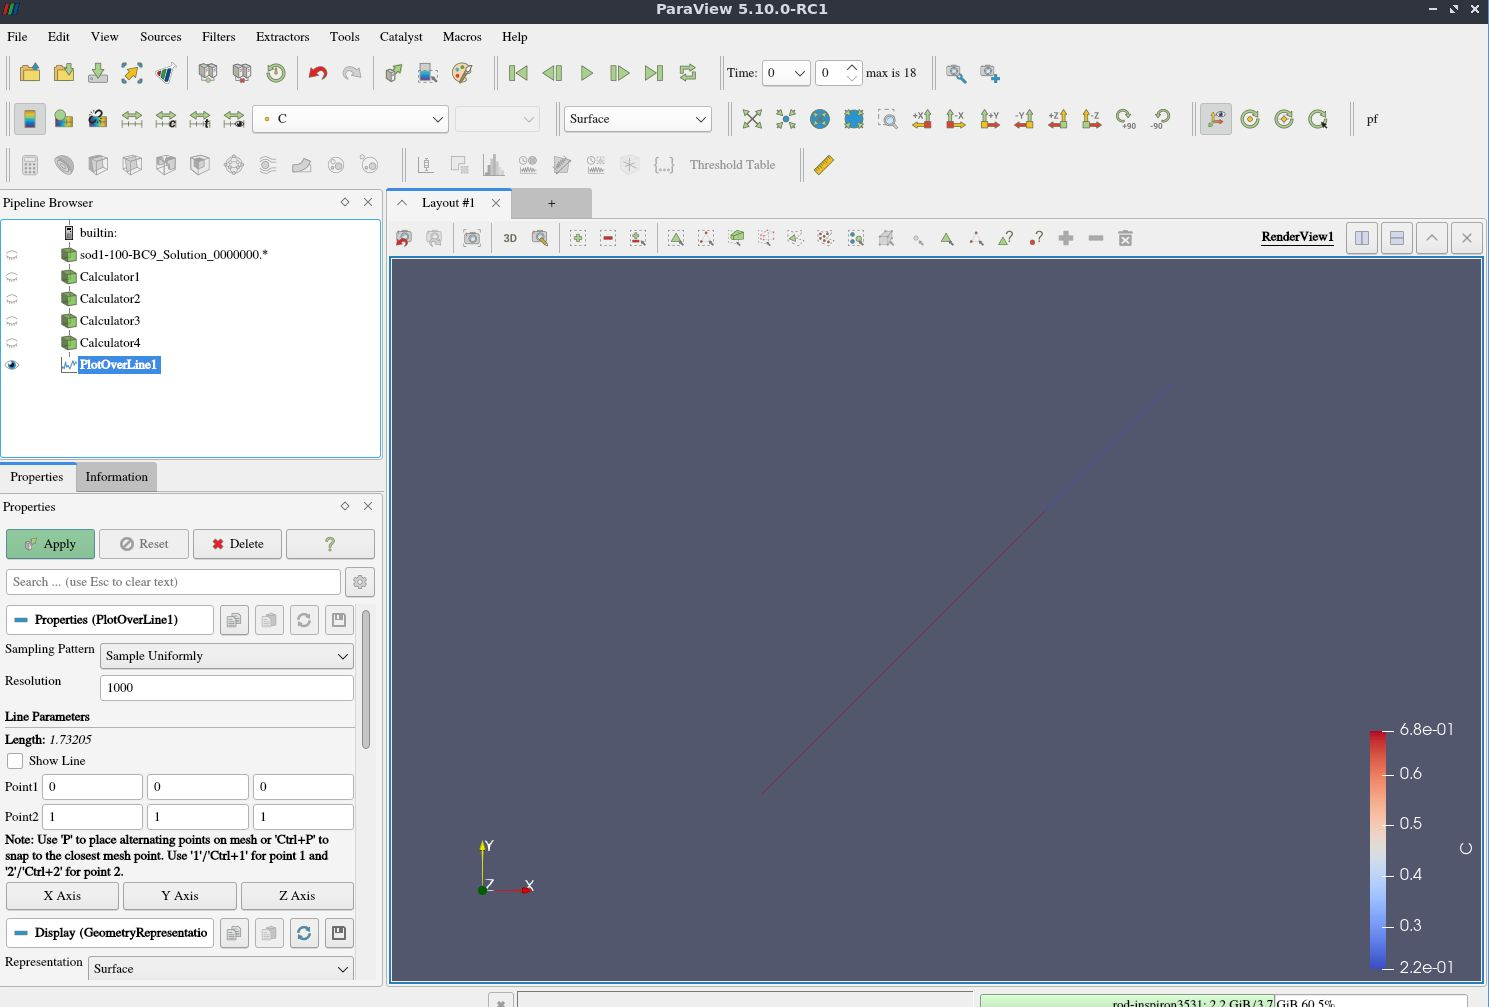
\includegraphics[width=.9\linewidth,height=0.9\linewidth,scale=1]{figures/paraviewGrabs/POL1.jpg}
  \caption{Use the Plot-Over-Line app to extract line plots of simulation data.}
  \label{fig:POL1}
\end{subfigure}
\begin{subfigure}{.95\textwidth}
  \centering
  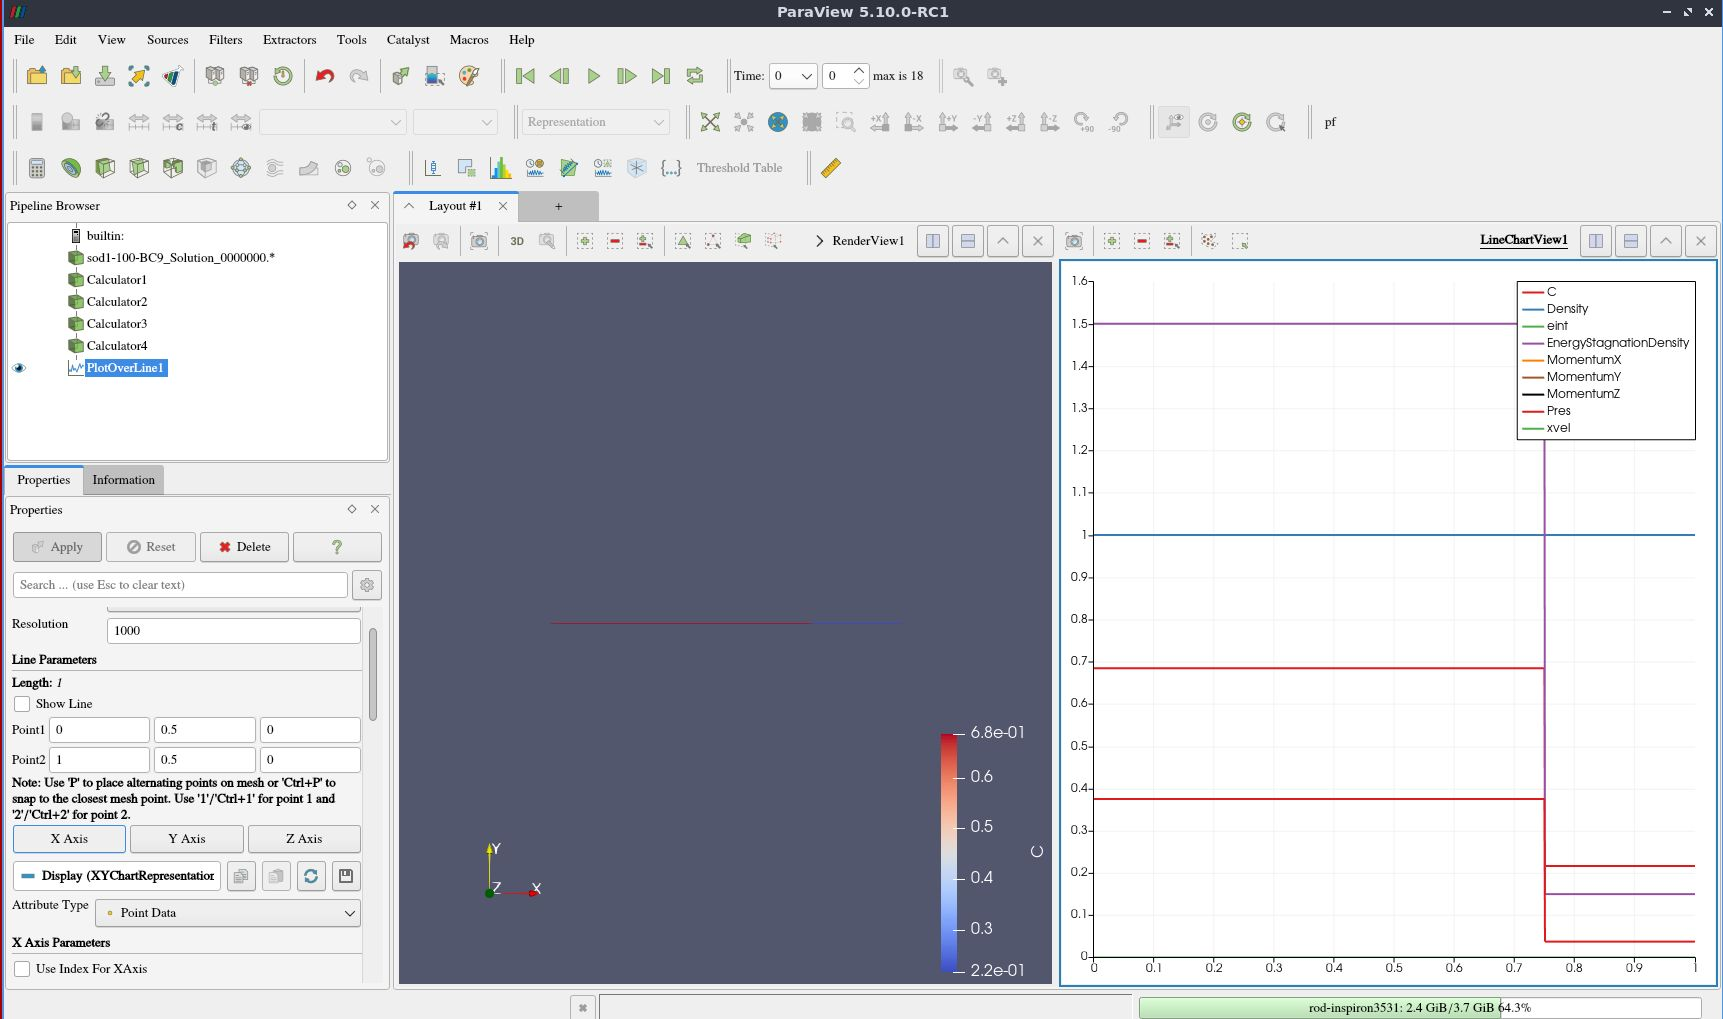
\includegraphics[width=.9\linewidth,height=0.9\linewidth,scale=1]{figures/paraviewGrabs/POL2.jpg}
  \caption{Use the Calculator app to calculate the specific internal energy.}
  \label{fig:POL2}
\end{subfigure}
\end{figure}
\begin{figure}\ContinuedFloat
\centering
\begin{subfigure}{.95\textwidth}
  \centering
  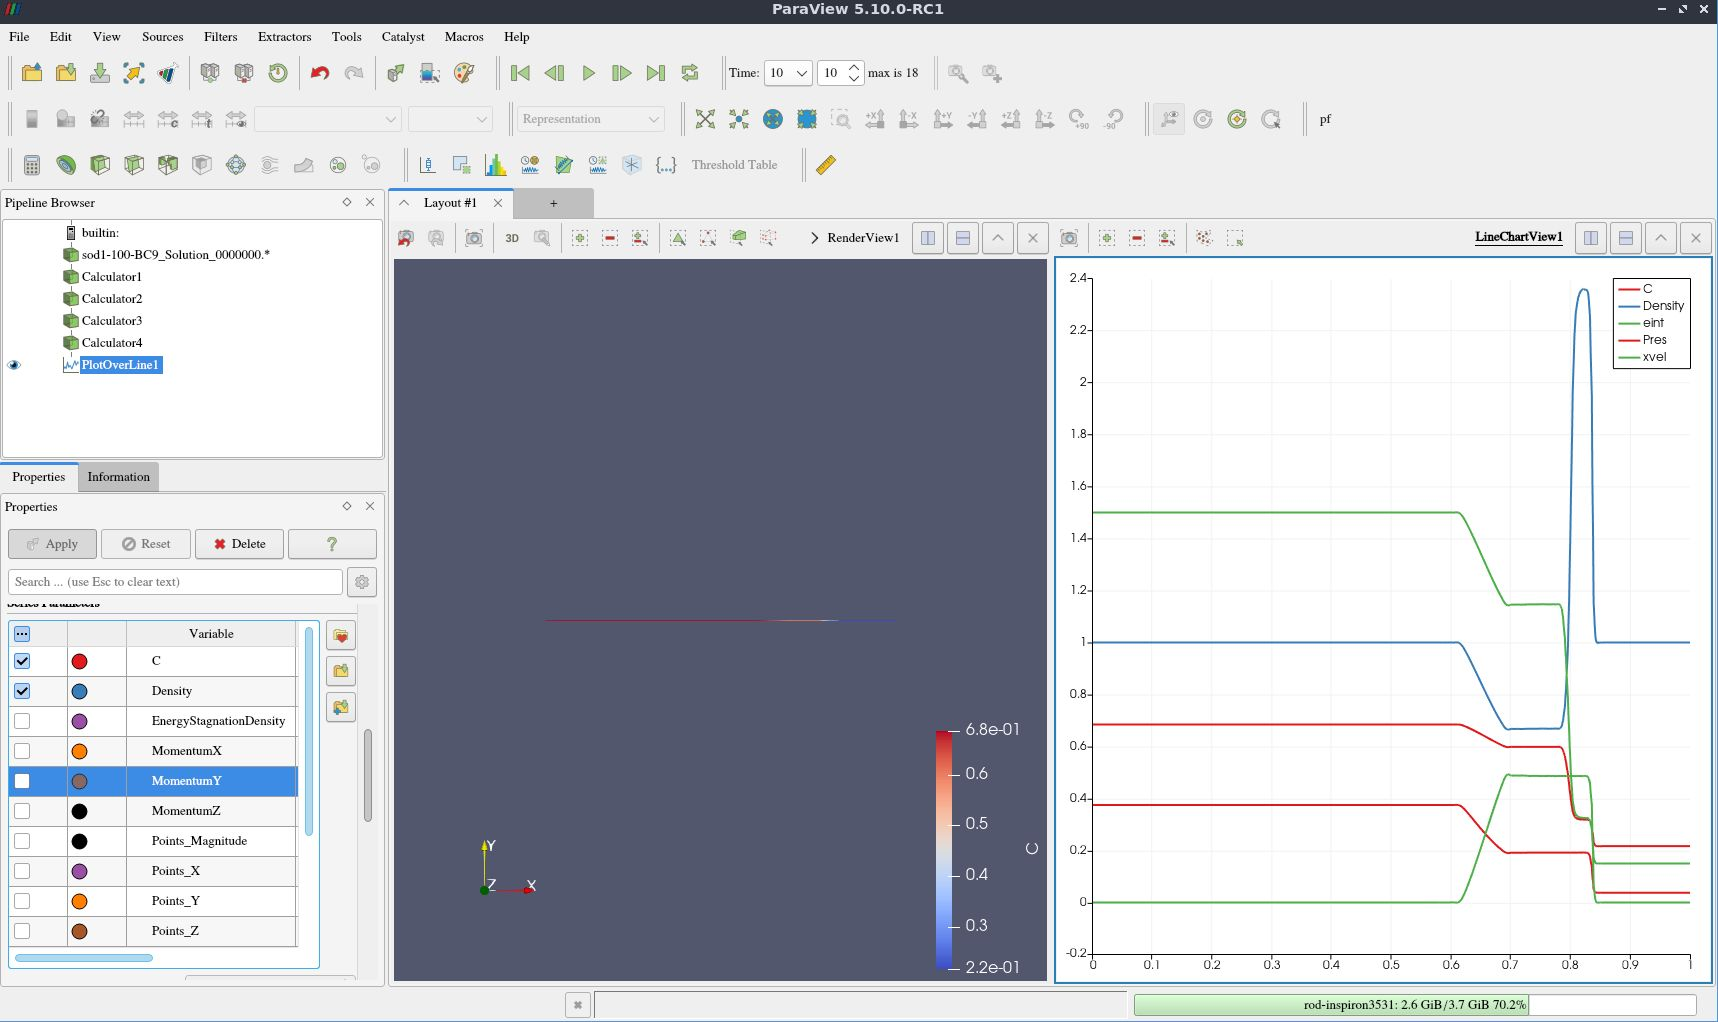
\includegraphics[width=.9\linewidth,height=0.9\linewidth,scale=1]{figures/paraviewGrabs/POL3.jpg}
  \caption{Use the Calculator app to calculate the pressure.}
  \label{fig:POL3}
\end{subfigure}
\begin{subfigure}{.95\textwidth}
  \centering
  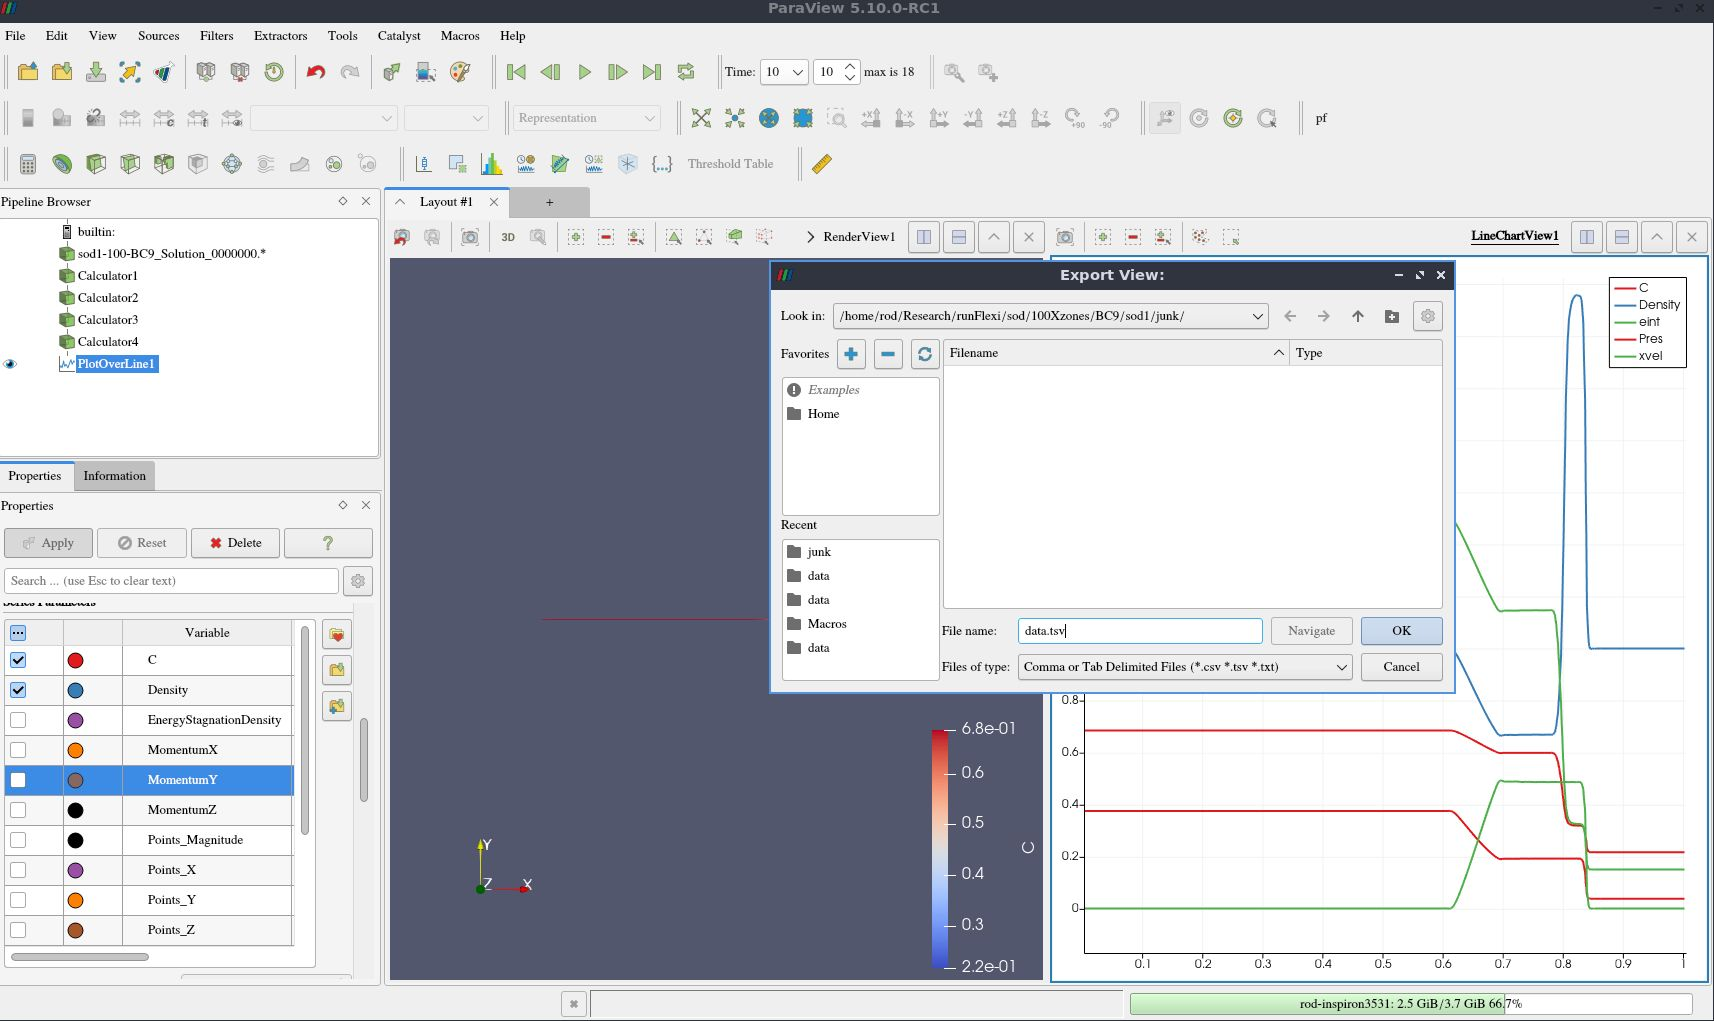
\includegraphics[width=.9\linewidth,height=0.9\linewidth,scale=1]{figures/paraviewGrabs/POL4.jpg}
  \caption{Use the Calculator app to calculate the speed of sound.}
  \label{fig:POL4}
\end{subfigure}
\caption{ParaView: Extracting line plots of simulation data and exporting numerical values for the plot data.}
\label{fig:POL}
\end{figure}

\section{Using xfig with PDF\LaTeX}\label{Asec:xfig}
\setcounter{figure}{0}

Using xfig\footnote{Using xfig version 3.2.8b with \LaTeX\  prepared using Kile version 2.9.93.  The computer operating system is Ubuntu 22.04.2 LTS} with PDF\LaTeX\  was done using the following process. Figure~\ref{fig:xfigRaw} shows a figure loaded into xfig with \LaTeX symbols  added to the figure in Text mode.  This drawing is then exported using the ''Combined PDF/\LaTeX (both parts)'' option, which generates the two files as discussed below.  The results after PDF\LaTeX processing are shown in Figure~\ref{fig:xfigLatex}.

\begin{enumerate}
 \item In xfig, create the desired drawing or load a ''.fig`` file
  \begin{enumerate}
   \item Locate on the drawing where text and/or symbols are to appear
   \item Using the \textbf{T} (TEXT input from keyboard) button,  click on the location
   where \LaTeX text is to appear.
   \item Enter the text as you would in a \LaTeX document
   \item Repeat as needed
   \item When finished with the drawing, save the figure
   \item Click on the File button and select ''export''
   \item From the ``Language'' menu select ``Combined PDF/\LaTeX (both parts)''
   \item In the ``Output file'' box, enter the file name (with the .pdf extension)
   \item In the ``Current Dir'' box, enter the  desired directory where the exported file  will be located
   \item The final figure size can be modified using the ``Magnification \%'' button
   \item Finally, click on the ``Export'' button on the bottom of the window
   \item xfig will ask if you want to save the figure.
   \item Answers ``Yes'' or ``No'' will result in 2 files being written to disk: \verb|outFileName.pdftex_t| and \verb|outFileName.pdftex|
  \end{enumerate}
\item In the document being prepared, create a figure environment (with centering if desired).  For example:

\begin{verbatim}
\begin{figure}[ht]
 \begin{center}
  \input{figures/shocktube.pdftex_t}
  \caption{Sod shock tube initial conditions.}
  \label{fig:shockICs}
 \end{center}
\end{figure}
\end{verbatim}

\noindent Note that the input file has the  ``pdftex\_t'' extension and is editable.  It contains the \verb|\includegraphics{shocktube.pdftex}| command and should be modified to give its correct path, in this case \\ \verb|\includegraphics{figures/shocktube.pdftex}|.
\end{enumerate}

\begin{figure}[h!]
\centering
\begin{subfigure}[h!]{\linewidth}
\centering
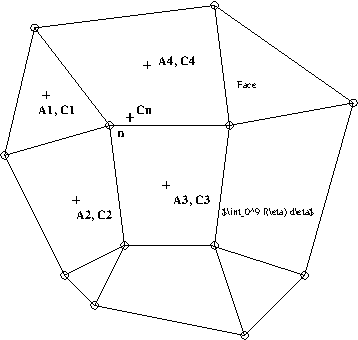
\includegraphics[scale=1.]{figures/CentPDF.pdf}
\caption{Using \LaTeX commands in xfig figure.}
  \label{fig:xfigRaw}
\end{subfigure}

\bigskip

\begin{subfigure}[h!]{\linewidth}
\centering
\input{figures/centLA.pdf_t}
\caption{\LaTeX processed figure.}
\label{fig:xfigLatex}
\end{subfigure}%
\caption{Using xfig with PDF\LaTeX.}
\end{figure}

\section{Flexi Input Files}\label{Asec:flexiinput}

\subsection{$\mathrm{sod}_1$ parameter\_flexi.ini File}\label{ssec:flexiin-sod1}
\verbatiminput{inputFiles/parameter_flexi-sod1.ini}

\subsection{$\mathrm{sod}_2$ Flexi Input: Free Boundaries}\label{ssec:flexiin-sod2-BC2}
\verbatiminput{inputFiles/parameter_flexi-sod2-BC2.ini}

\subsection{$\mathrm{sod}_2$ Flexi Input: Symmetry Boundaries}\label{ssec:flexiin-sod2-BC9}
\verbatiminput{inputFiles/parameter_flexi-sod2-BC9.ini}

\subsection{$\mathrm{sod}_3$ Flexi Input: Free Boundaries}\label{ssec:flexiin-sod3-BC9}
\verbatiminput{inputFiles/parameter_flexi-sod3-BC9.ini}

\subsection{Einfeldt 123-Problem Flexi Input}\label{ssec:flexiin-einfeldt}
\verbatiminput{inputFiles/parameter_flexi-einfeldt.ini}

\subsection{LeBlanc-Problem Flexi Input}\label{ssec:flexiin-leblanc}
\verbatiminput{inputFiles/parameter_flexi-leblanc.ini}

\subsection{Sedov-Problem Flexi Input}\label{ssec:flexiin-sedov}
\verbatiminput{inputFiles/parameter_flexi-sedov.ini}

\subsection{Hui Problem ($\beta = 0$) Flexi Input}\label{ssec:flexiin-hui-Rot0}
\verbatiminput{inputFiles/parameter_flexi-hui-Rot0.ini}

\subsection{Hui Problem ($\beta = 0.4$) Flexi Input}\label{ssec:flexiin-hui-Rot}
\verbatiminput{inputFiles/parameter_flexi-hui-Rot.ini}


\section{HOPR Input Files}\label{Asec:hoprinput}

\subsection{$\mathrm{sod}_1$ HOPR Input}\label{ssec:hoprin-sod1}
\verbatiminput{inputFiles/parameter_hopr-sod1.ini}

\subsection{$\mathrm{sod}_2$ HOPR Input: Inflow/Outflow Boundaries}\label{ssec:hoprin-sod2-BC2}
\verbatiminput{inputFiles/parameter_hopr-sod2-BC2.ini}

\subsection{$\mathrm{sod}_2$ HOPR Input: Symmetry Boundaries}\label{ssec:hoprin-sod2-BC9}
\verbatiminput{inputFiles/parameter_hopr-sod2-BC9.ini}

\subsection{$\mathrm{sod}_3$ HOPR Input: Inflow/Outflow Boundaries}\label{ssec:hoprin-sod3-BC9}
\verbatiminput{inputFiles/parameter_hopr-sod3-BC9.ini}

\subsection{Einfeldt 123-problem HOPR Input: Inflow/Outflow Boundaries}\label{ssec:hoprin-einfeldt}
\verbatiminput{inputFiles/parameter_hopr-einfeldt.ini}

\subsection{LeBlanc Problem HOPR Input}\label{ssec:hoprin-leblanc}
\verbatiminput{inputFiles/parameter_hopr-leblanc.ini}

\subsection{Sedov-Problem HOPR Input}\label{ssec:hoprin-sedov}
\verbatiminput{inputFiles/parameter_hopr-sedov.ini}

\subsection{Hui Problem ($\beta = 0$) HOPR Input}\label{ssec:hoprin-hui-Rot0}
\verbatiminput{inputFiles/parameter_hopr-hui-Rot0.ini}

\subsection{Hui Problem ($\beta = 0.4$) HOPR Input}\label{ssec:hoprin-hui-Rot}
\verbatiminput{inputFiles/parameter_hopr-hui-Rot.ini}

\end{appendices}


\bibliography{flexiReferences}

\end{document}
